\documentclass[12pt,a4paper,]{book}
\def\ifdoblecara{} %% set to true
\def\ifprincipal{} %% set to true
\def\ifcitapandoc{} %% set to true
\let\ifcitapandoc\undefined %% set to false
\usepackage{lmodern}
\usepackage{amssymb,amsmath}
\usepackage{ifxetex,ifluatex}
%\usepackage{fixltx2e} % provides \textsubscript %PLLC
\ifnum 0\ifxetex 1\fi\ifluatex 1\fi=0 % if pdftex
  \usepackage[T1]{fontenc}
  \usepackage[utf8]{inputenc}
\else % if luatex or xelatex
  \ifxetex
    \usepackage{mathspec}
  \else
    \usepackage{fontspec}
  \fi
  \defaultfontfeatures{Ligatures=TeX,Scale=MatchLowercase}
\fi
% use upquote if available, for straight quotes in verbatim environments
\IfFileExists{upquote.sty}{\usepackage{upquote}}{}
% use microtype if available
\IfFileExists{microtype.sty}{%
\usepackage{microtype}
\UseMicrotypeSet[protrusion]{basicmath} % disable protrusion for tt fonts
}{}
\usepackage[margin = 2.5cm]{geometry}
\usepackage{hyperref}
\hypersetup{unicode=true,
              pdfborder={0 0 0},
              breaklinks=true}
\urlstyle{same}  % don't use monospace font for urls
\usepackage{natbib}
\bibliographystyle{plainnat}
\usepackage[usenames,dvipsnames]{xcolor}  %new PLLC
\IfFileExists{parskip.sty}{%
\usepackage{parskip}
}{% else
\setlength{\parindent}{0pt}
\setlength{\parskip}{6pt plus 2pt minus 1pt}
}
\setlength{\emergencystretch}{3em}  % prevent overfull lines
\providecommand{\tightlist}{%
  \setlength{\itemsep}{0pt}\setlength{\parskip}{0pt}}
\setcounter{secnumdepth}{5}
% Redefines (sub)paragraphs to behave more like sections
\ifx\paragraph\undefined\else
\let\oldparagraph\paragraph
\renewcommand{\paragraph}[1]{\oldparagraph{#1}\mbox{}}
\fi
\ifx\subparagraph\undefined\else
\let\oldsubparagraph\subparagraph
\renewcommand{\subparagraph}[1]{\oldsubparagraph{#1}\mbox{}}
\fi

%%% Use protect on footnotes to avoid problems with footnotes in titles
\let\rmarkdownfootnote\footnote%
\def\footnote{\protect\rmarkdownfootnote}


  \title{}
    \author{}
    \date{}
  

%%%%%%% inicio: latex_preambulo.tex PLLC

%% UTILIZA CODIFICACIÓN UTF-8
%% MODIFICARLO CONVENIENTEMENTE PARA USARLO CON OTRAS CODIFICACIONES


\usepackage[spanish,es-nodecimaldot,es-noshorthands]{babel}
\usepackage{float}
\usepackage{placeins}
\usepackage{fancyhdr}
% Solucion: ! LaTeX Error: Command \counterwithout already defined.
% https://tex.stackexchange.com/questions/425600/latex-error-command-counterwithout-already-defined
\let\counterwithout\relax
\let\counterwithin\relax
\usepackage{chngcntr}
%\usepackage{microtype}  %antes en template PLLC
\usepackage[utf8]{inputenc}
\usepackage[T1]{fontenc} % Usa codificación 8-bit que tiene 256 glyphs

%\usepackage[dvipsnames]{xcolor}
%\usepackage[usenames,dvipsnames]{xcolor}  %new
\usepackage{pdfpages}
%\usepackage{natbib}




% Para portada: latex_paginatitulo_mod_ST02.tex (inicio)
\usepackage{tikz}
\usepackage{epigraph}
\renewcommand\epigraphflush{flushright}
\renewcommand\epigraphsize{\normalsize}
\setlength\epigraphwidth{0.7\textwidth}

\definecolor{titlepagecolor}{cmyk}{1,.60,0,.40}

%\DeclareFixedFont{\titlefont}{T1}{ppl}{b}{it}{0.5in}

% \makeatletter
% \def\printauthor{%
%     {\large \@author}}
% \makeatother
% \author{%
%     Author 1 name \\
%     Department name \\
%     \texttt{email1@example.com}\vspace{20pt} \\
%     Author 2 name \\
%     Department name \\
%     \texttt{email2@example.com}
%     }

% The following code is borrowed from: https://tex.stackexchange.com/a/86310/10898

\newcommand\titlepagedecoration{%
\begin{tikzpicture}[remember picture,overlay,shorten >= -10pt]

\coordinate (aux1) at ([yshift=-15pt]current page.north east);
\coordinate (aux2) at ([yshift=-410pt]current page.north east);
\coordinate (aux3) at ([xshift=-4.5cm]current page.north east);
\coordinate (aux4) at ([yshift=-150pt]current page.north east);

\begin{scope}[titlepagecolor!40,line width=12pt,rounded corners=12pt]
\draw
  (aux1) -- coordinate (a)
  ++(225:5) --
  ++(-45:5.1) coordinate (b);
\draw[shorten <= -10pt]
  (aux3) --
  (a) --
  (aux1);
\draw[opacity=0.6,titlepagecolor,shorten <= -10pt]
  (b) --
  ++(225:2.2) --
  ++(-45:2.2);
\end{scope}
\draw[titlepagecolor,line width=8pt,rounded corners=8pt,shorten <= -10pt]
  (aux4) --
  ++(225:0.8) --
  ++(-45:0.8);
\begin{scope}[titlepagecolor!70,line width=6pt,rounded corners=8pt]
\draw[shorten <= -10pt]
  (aux2) --
  ++(225:3) coordinate[pos=0.45] (c) --
  ++(-45:3.1);
\draw
  (aux2) --
  (c) --
  ++(135:2.5) --
  ++(45:2.5) --
  ++(-45:2.5) coordinate[pos=0.3] (d);   
\draw 
  (d) -- +(45:1);
\end{scope}
\end{tikzpicture}%
}

% Para portada: latex_paginatitulo_mod_ST02.tex (fin)

% Para portada: latex_paginatitulo_mod_OV01.tex (inicio)
\usepackage{cpimod}
% Para portada: latex_paginatitulo_mod_OV01.tex (fin)

% Para portada: latex_paginatitulo_mod_OV03.tex (inicio)
\usepackage{KTHEEtitlepage}
% Para portada: latex_paginatitulo_mod_OV03.tex (fin)

\renewcommand{\contentsname}{Índice}
\renewcommand{\listfigurename}{Índice de figuras}
\renewcommand{\listtablename}{Índice de tablas}
\newcommand{\bcols}{}
\newcommand{\ecols}{}
\newcommand{\bcol}[1]{\begin{minipage}{#1\linewidth}}
\newcommand{\ecol}{\end{minipage}}
\newcommand{\balertblock}[1]{\begin{alertblock}{#1}}
\newcommand{\ealertblock}{\end{alertblock}}
\newcommand{\bitemize}{\begin{itemize}}
\newcommand{\eitemize}{\end{itemize}}
\newcommand{\benumerate}{\begin{enumerate}}
\newcommand{\eenumerate}{\end{enumerate}}
\newcommand{\saltopagina}{\newpage}
\newcommand{\bcenter}{\begin{center}}
\newcommand{\ecenter}{\end{center}}
\newcommand{\beproof}{\begin{proof}} %new
\newcommand{\eeproof}{\end{proof}} %new
%De: https://texblog.org/2007/11/07/headerfooter-in-latex-with-fancyhdr/
% \fancyhead
% E: Even page
% O: Odd page
% L: Left field
% C: Center field
% R: Right field
% H: Header
% F: Footer
%\fancyhead[CO,CE]{Resultados}

%OPCION 1
% \fancyhead[LE,RO]{\slshape \rightmark}
% \fancyhead[LO,RE]{\slshape \leftmark}
% \fancyfoot[C]{\thepage}
% \renewcommand{\headrulewidth}{0.4pt}
% \renewcommand{\footrulewidth}{0pt}

%OPCION 2
% \fancyhead[LE,RO]{\slshape \rightmark}
% \fancyfoot[LO,RE]{\slshape \leftmark}
% \fancyfoot[LE,RO]{\thepage}
% \renewcommand{\headrulewidth}{0.4pt}
% \renewcommand{\footrulewidth}{0.4pt}
%%%%%%%%%%
\usepackage{calc,amsfonts}
% Elimina la cabecera de páginas impares vacías al finalizar los capítulos
\usepackage{emptypage}
\makeatletter

\definecolor{ocre}{RGB}{25,25,243} % Define el color naranja usado para resaltar algunas salidas

%\usepackage{calc} 

\usepackage{lipsum}

%\usepackage{tikz} % Requerido para dibujar formas personalizadas

%\usepackage{amsmath,amsthm,amssymb,amsfonts}
\usepackage{amsthm}


% Boxed/framed environments
\newtheoremstyle{ocrenumbox}% % Theorem style name
{0pt}% Space above
{0pt}% Space below
{\normalfont}% % Body font
{}% Indent amount
{\small\bf\sffamily\color{ocre}}% % Theorem head font
{\;}% Punctuation after theorem head
{0.25em}% Space after theorem head
{\small\sffamily\color{ocre}\thmname{#1}\nobreakspace\thmnumber{\@ifnotempty{#1}{}\@upn{#2}}% Theorem text (e.g. Theorem 2.1)
\thmnote{\nobreakspace\the\thm@notefont\sffamily\bfseries\color{black}---\nobreakspace#3.}} % Optional theorem note
\renewcommand{\qedsymbol}{$\blacksquare$}% Optional qed square

\newtheoremstyle{blacknumex}% Theorem style name
{5pt}% Space above
{5pt}% Space below
{\normalfont}% Body font
{} % Indent amount
{\small\bf\sffamily}% Theorem head font
{\;}% Punctuation after theorem head
{0.25em}% Space after theorem head
{\small\sffamily{\tiny\ensuremath{\blacksquare}}\nobreakspace\thmname{#1}\nobreakspace\thmnumber{\@ifnotempty{#1}{}\@upn{#2}}% Theorem text (e.g. Theorem 2.1)
\thmnote{\nobreakspace\the\thm@notefont\sffamily\bfseries---\nobreakspace#3.}}% Optional theorem note

\newtheoremstyle{blacknumbox} % Theorem style name
{0pt}% Space above
{0pt}% Space below
{\normalfont}% Body font
{}% Indent amount
{\small\bf\sffamily}% Theorem head font
{\;}% Punctuation after theorem head
{0.25em}% Space after theorem head
{\small\sffamily\thmname{#1}\nobreakspace\thmnumber{\@ifnotempty{#1}{}\@upn{#2}}% Theorem text (e.g. Theorem 2.1)
\thmnote{\nobreakspace\the\thm@notefont\sffamily\bfseries---\nobreakspace#3.}}% Optional theorem note

% Non-boxed/non-framed environments
\newtheoremstyle{ocrenum}% % Theorem style name
{5pt}% Space above
{5pt}% Space below
{\normalfont}% % Body font
{}% Indent amount
{\small\bf\sffamily\color{ocre}}% % Theorem head font
{\;}% Punctuation after theorem head
{0.25em}% Space after theorem head
{\small\sffamily\color{ocre}\thmname{#1}\nobreakspace\thmnumber{\@ifnotempty{#1}{}\@upn{#2}}% Theorem text (e.g. Theorem 2.1)
\thmnote{\nobreakspace\the\thm@notefont\sffamily\bfseries\color{black}---\nobreakspace#3.}} % Optional theorem note
\renewcommand{\qedsymbol}{$\blacksquare$}% Optional qed square
\makeatother



% Define el estilo texto theorem para cada tipo definido anteriormente
\newcounter{dummy} 
\numberwithin{dummy}{section}
\theoremstyle{ocrenumbox}
\newtheorem{theoremeT}[dummy]{Teorema}  % (Pedro: Theorem)
\newtheorem{problem}{Problema}[chapter]  % (Pedro: Problem)
\newtheorem{exerciseT}{Ejercicio}[chapter] % (Pedro: Exercise)
\theoremstyle{blacknumex}
\newtheorem{exampleT}{Ejemplo}[chapter] % (Pedro: Example)
\theoremstyle{blacknumbox}
\newtheorem{vocabulary}{Vocabulario}[chapter]  % (Pedro: Vocabulary)
\newtheorem{definitionT}{Definición}[section]  % (Pedro: Definition)
\newtheorem{corollaryT}[dummy]{Corolario}  % (Pedro: Corollary)
\theoremstyle{ocrenum}
\newtheorem{proposition}[dummy]{Proposición} % (Pedro: Proposition)


\usepackage[framemethod=default]{mdframed}



\newcommand{\intoo}[2]{\mathopen{]}#1\,;#2\mathclose{[}}
\newcommand{\ud}{\mathop{\mathrm{{}d}}\mathopen{}}
\newcommand{\intff}[2]{\mathopen{[}#1\,;#2\mathclose{]}}
\newtheorem{notation}{Notation}[chapter]


\mdfdefinestyle{exampledefault}{%
rightline=true,innerleftmargin=10,innerrightmargin=10,
frametitlerule=true,frametitlerulecolor=green,
frametitlebackgroundcolor=yellow,
frametitlerulewidth=2pt}


% Theorem box
\newmdenv[skipabove=7pt,
skipbelow=7pt,
backgroundcolor=black!5,
linecolor=ocre,
innerleftmargin=5pt,
innerrightmargin=5pt,
innertopmargin=10pt,%5pt
leftmargin=0cm,
rightmargin=0cm,
innerbottommargin=5pt]{tBox}

% Exercise box	  
\newmdenv[skipabove=7pt,
skipbelow=7pt,
rightline=false,
leftline=true,
topline=false,
bottomline=false,
backgroundcolor=ocre!10,
linecolor=ocre,
innerleftmargin=5pt,
innerrightmargin=5pt,
innertopmargin=10pt,%5pt
innerbottommargin=5pt,
leftmargin=0cm,
rightmargin=0cm,
linewidth=4pt]{eBox}	

% Definition box
\newmdenv[skipabove=7pt,
skipbelow=7pt,
rightline=false,
leftline=true,
topline=false,
bottomline=false,
linecolor=ocre,
innerleftmargin=5pt,
innerrightmargin=5pt,
innertopmargin=10pt,%0pt
leftmargin=0cm,
rightmargin=0cm,
linewidth=4pt,
innerbottommargin=0pt]{dBox}	

% Corollary box
\newmdenv[skipabove=7pt,
skipbelow=7pt,
rightline=false,
leftline=true,
topline=false,
bottomline=false,
linecolor=gray,
backgroundcolor=black!5,
innerleftmargin=5pt,
innerrightmargin=5pt,
innertopmargin=10pt,%5pt
leftmargin=0cm,
rightmargin=0cm,
linewidth=4pt,
innerbottommargin=5pt]{cBox}

% Crea un entorno para cada tipo de theorem y le asigna un estilo 
% con ayuda de las cajas coloreadas anteriores
\newenvironment{theorem}{\begin{tBox}\begin{theoremeT}}{\end{theoremeT}\end{tBox}}
\newenvironment{exercise}{\begin{eBox}\begin{exerciseT}}{\hfill{\color{ocre}\tiny\ensuremath{\blacksquare}}\end{exerciseT}\end{eBox}}				  
\newenvironment{definition}{\begin{dBox}\begin{definitionT}}{\end{definitionT}\end{dBox}}	
\newenvironment{example}{\begin{exampleT}}{\hfill{\tiny\ensuremath{\blacksquare}}\end{exampleT}}		
\newenvironment{corollary}{\begin{cBox}\begin{corollaryT}}{\end{corollaryT}\end{cBox}}	

%	ENVIRONMENT remark
\newenvironment{remark}{\par\vspace{10pt}\small 
% Espacio blanco vertical sobre la nota y tamaño de fuente menor
\begin{list}{}{
\leftmargin=35pt % Indentación sobre la izquierda
\rightmargin=25pt}\item\ignorespaces % Indentación sobre la derecha
\makebox[-2.5pt]{\begin{tikzpicture}[overlay]
\node[draw=ocre!60,line width=1pt,circle,fill=ocre!25,font=\sffamily\bfseries,inner sep=2pt,outer sep=0pt] at (-15pt,0pt){\textcolor{ocre}{N}}; \end{tikzpicture}} % R naranja en un círculo (Pedro)
\advance\baselineskip -1pt}{\end{list}\vskip5pt} 
% Espaciado de línea más estrecho y espacio en blanco después del comentario


\newenvironment{solutionExe}{\par\vspace{10pt}\small 
\begin{list}{}{
\leftmargin=35pt 
\rightmargin=25pt}\item\ignorespaces 
\makebox[-2.5pt]{\begin{tikzpicture}[overlay]
\node[draw=ocre!60,line width=1pt,circle,fill=ocre!25,font=\sffamily\bfseries,inner sep=2pt,outer sep=0pt] at (-15pt,0pt){\textcolor{ocre}{S}}; \end{tikzpicture}} 
\advance\baselineskip -1pt}{\end{list}\vskip5pt} 

\newenvironment{solutionExa}{\par\vspace{10pt}\small 
\begin{list}{}{
\leftmargin=35pt 
\rightmargin=25pt}\item\ignorespaces 
\makebox[-2.5pt]{\begin{tikzpicture}[overlay]
\node[draw=ocre!60,line width=1pt,circle,fill=ocre!55,font=\sffamily\bfseries,inner sep=2pt,outer sep=0pt] at (-15pt,0pt){\textcolor{ocre}{S}}; \end{tikzpicture}} 
\advance\baselineskip -1pt}{\end{list}\vskip5pt} 

\usepackage{tcolorbox}

\usetikzlibrary{trees}

\theoremstyle{ocrenum}
\newtheorem{solutionT}[dummy]{Solución}  % (Pedro: Corollary)
\newenvironment{solution}{\begin{cBox}\begin{solutionT}}{\end{solutionT}\end{cBox}}	


\newcommand{\tcolorboxsolucion}[2]{%
\begin{tcolorbox}[colback=green!5!white,colframe=green!75!black,title=#1] 
 #2
 %\tcblower  % pone una línea discontinua
\end{tcolorbox}
}% final definición comando

\newtcbox{\mybox}[1][green]{on line,
arc=0pt,outer arc=0pt,colback=#1!10!white,colframe=#1!50!black, boxsep=0pt,left=1pt,right=1pt,top=2pt,bottom=2pt, boxrule=0pt,bottomrule=1pt,toprule=1pt}



\mdfdefinestyle{exampledefault}{%
rightline=true,innerleftmargin=10,innerrightmargin=10,
frametitlerule=true,frametitlerulecolor=green,
frametitlebackgroundcolor=yellow,
frametitlerulewidth=2pt}





\newcommand{\betheorem}{\begin{theorem}}
\newcommand{\eetheorem}{\end{theorem}}
\newcommand{\bedefinition}{\begin{definition}}
\newcommand{\eedefinition}{\end{definition}}

\newcommand{\beremark}{\begin{remark}}
\newcommand{\eeremark}{\end{remark}}
\newcommand{\beexercise}{\begin{exercise}}
\newcommand{\eeexercise}{\end{exercise}}
\newcommand{\beexample}{\begin{example}}
\newcommand{\eeexample}{\end{example}}
\newcommand{\becorollary}{\begin{corollary}}
\newcommand{\eecorollary}{\end{corollary}}


\newcommand{\besolutionExe}{\begin{solutionExe}}
\newcommand{\eesolutionExe}{\end{solutionExe}}
\newcommand{\besolutionExa}{\begin{solutionExa}}
\newcommand{\eesolutionExa}{\end{solutionExa}}


%%%%%%%%


% Caja Salida Markdown
\newmdenv[skipabove=7pt,
skipbelow=7pt,
rightline=false,
leftline=true,
topline=false,
bottomline=false,
backgroundcolor=GreenYellow!10,
linecolor=GreenYellow!80,
innerleftmargin=5pt,
innerrightmargin=5pt,
innertopmargin=10pt,%5pt
innerbottommargin=5pt,
leftmargin=0cm,
rightmargin=0cm,
linewidth=4pt]{mBox}	

%% RMarkdown
\newenvironment{markdownsal}{\begin{mBox}}{\end{mBox}}	

\newcommand{\bmarkdownsal}{\begin{markdownsal}}
\newcommand{\emarkdownsal}{\end{markdownsal}}


\usepackage{array}
\usepackage{multirow}
\usepackage{wrapfig}
\usepackage{colortbl}
\usepackage{pdflscape}
\usepackage{tabu}
\usepackage{threeparttable}
\usepackage{subfig} %new
%\usepackage{booktabs,dcolumn,rotating,thumbpdf,longtable}
\usepackage{dcolumn,rotating}  %new
\usepackage[graphicx]{realboxes} %new de: https://stackoverflow.com/questions/51633434/prevent-pagebreak-in-kableextra-landscape-table

%define el interlineado vertical
%\renewcommand{\baselinestretch}{1.5}

%define etiqueta para las Tablas o Cuadros
%\renewcommand\spanishtablename{Tabla}

%%\bibliographystyle{plain} %new no necesario


%%%%%%%%%%%% PARA USO CON biblatex
% \DefineBibliographyStrings{english}{%
%   backrefpage = {ver pag.\adddot},%
%   backrefpages = {ver pags.\adddot}%
% }

% \DefineBibliographyStrings{spanish}{%
%   backrefpage = {ver pag.\adddot},%
%   backrefpages = {ver pags.\adddot}%
% }
% 
% \DeclareFieldFormat{pagerefformat}{\mkbibparens{{\color{red}\mkbibemph{#1}}}}
% \renewbibmacro*{pageref}{%
%   \iflistundef{pageref}
%     {}
%     {\printtext[pagerefformat]{%
%        \ifnumgreater{\value{pageref}}{1}
%          {\bibstring{backrefpages}\ppspace}
%          {\bibstring{backrefpage}\ppspace}%
%        \printlist[pageref][-\value{listtotal}]{pageref}}}}
% 
%%% de kableExtra
\usepackage{booktabs}
\usepackage{longtable}
%\usepackage{array}
%\usepackage{multirow}
%\usepackage{wrapfig}
%\usepackage{float}
%\usepackage{colortbl}
%\usepackage{pdflscape}
%\usepackage{tabu}
%\usepackage{threeparttable}
\usepackage{threeparttablex}
\usepackage[normalem]{ulem}
\usepackage{makecell}
%\usepackage{xcolor}

%%%%%%% fin: latex_preambulo.tex PLLC




\begin{document}

% nada
\begin{titlepage}

\newcommand{\HRule}{\rule{\linewidth}{0.5mm}} % Defines a new command for the horizontal lines, change thickness here

\center % Center everything on the page


\begin{minipage}{14cm}
%----------------------------------------------------------------------------------------
%  LOGO SECTION
%----------------------------------------------------------------------------------------
\center


\includegraphics[width=8cm,height=8cm]{logo}\\[0.5cm] % Include a department/university logo - this will require the graphicx package

%----------------------------------------------------------------------------------------

%----------------------------------------------------------------------------------------
%	HEADING SECTIONS
%----------------------------------------------------------------------------------------
\textsc{\LARGE Grado en Estadística}\\[2.5cm] 


%----------------------------------------------------------------------------------------
%	TITLE SECTION
%----------------------------------------------------------------------------------------

\rule[1.7mm]{2cm}{0.5mm}
\hfill
\textsc{\Large TRABAJO FIN DE GRADO} 
\hfill
\rule[1.7mm]{2cm}{0.5mm} 
\\[0.75cm]

%\bfseries
{\Huge
\textbf{\textit{
Influencia de los métodos \\[0.2cm]
de reparto de escaños \\[0.5cm]
en los resultados electorales
}}}\\[0.75cm] 

\HRule \\[4cm]


{\Large

Angel González Rizo} \\[0.5cm]

{\large
Sevilla, Enero de 2020
}

\end{minipage}

\vfill % Fill the rest of the page with whitespace

\cleardoublepage
%\newpage{\ }
\thispagestyle{empty}
\end{titlepage}

\raggedbottom

\setlength{\parindent}{1em}

\pagestyle{fancy}
\ifdefined\ifdoblecara
\fancyhead[LE,RO]{}
\fancyhead[LO,RE]{}
\else
\fancyhead[RO]{}
\fancyhead[LO]{}
\fi
\renewcommand{\headrulewidth}{0pt}
\renewcommand{\footrulewidth}{0pt}
\pagenumbering{roman}

\setcounter{tocdepth}{2}
\subpdfbookmark{Índice General}{indice}
\tableofcontents

\cleardoublepage

\section*{Resumen}
\addcontentsline{toc}{section}{Resumen}

En este trabajo de fin de grado se ha tratado de analizar los distintos
métodos de repartición de escaños, enfocándolo desde una perspectiva
novedosa en donde se analizan los métodos variando experimentalmente los
escaños a repartir, el número de partidos que se presentan a la elección
o la concentración del voto. También se analiza el grado de
disproporcionalidad que resulta de haber realizado las elecciones en
España según los distintos métodos de reparto de escaños.

\clearpage
\section*{Abstract}
\addcontentsline{toc}{section}{Abstract}

In this end-of-degree work, we have tried to analyse the different
methods of distributing seats, focusing on them from a novel perspective
where the methods are analysed by experimentally varying the seats to be
distributed, the number of parties running for election or the
concentration of the vote. It also analyses the degree of
disproportionality resulting from having held elections in Spain
according to the different methods of seat distribution.

\cleardoublepage

\pagenumbering{arabic}

\ifdefined\ifdoblecara
\fancyhead[LE,RO]{\scriptsize\rightmark}
\fancyfoot[LO,RE]{\scriptsize\slshape \leftmark}
\fancyfoot[C]{}
\fancyfoot[LE,RO]{\footnotesize\thepage}
\else
\fancyhead[RO]{\scriptsize\rightmark}
\fancyfoot[LO]{\scriptsize\slshape \leftmark}
\fancyfoot[C]{}
\fancyfoot[RO]{\footnotesize\thepage}
\fi

\renewcommand{\headrulewidth}{0.4pt}
\renewcommand{\footrulewidth}{0.4pt}

\ifdefined\ifprincipal
\else
\setlength{\parindent}{1em}
\pagestyle{fancy}
\setcounter{tocdepth}{4}
\tableofcontents

\fi

\ifdefined\ifdoblecara
\fancyhead{}{}
\fancyhead[LE,RO]{\scriptsize\rightmark}
\fancyfoot[LO,RE]{\scriptsize\slshape \leftmark}
\fancyfoot[C]{}
\fancyfoot[LE,RO]{\footnotesize\thepage}
\else
\fancyhead{}{}
\fancyhead[RO]{\scriptsize\rightmark}
\fancyfoot[LO]{\scriptsize\slshape \leftmark}
\fancyfoot[C]{}
\fancyfoot[RO]{\footnotesize\thepage}
\fi
\renewcommand{\headrulewidth}{0.4pt}
\renewcommand{\footrulewidth}{0.4pt}

\hypertarget{introducciuxf3n}{%
\chapter{Introducción}\label{introducciuxf3n}}

\hypertarget{objetivos}{%
\section{Objetivos}\label{objetivos}}

Rev-El objetivo del presente trabajo será analizar los distintos
sistemas de votación que existen en la actualidad que puedan ser
aplicados actualmente en España, aplicar estos sistemas a España,
indicando sus ventajas e inconvenientes y proponer nuevos sistemas de
votación o reparto para una eventual reforma de la Ley Orgánica del
Régimen Electoral.

\hypertarget{quuxe9-significa-votar}{%
\section{¿Qué significa votar?}\label{quuxe9-significa-votar}}

\hypertarget{origen}{%
\subsection{Origen}\label{origen}}

Según la Real Academia de la Lengua Española votar proviene de la
palabra latina votare (hacer votos, hacer ofrendas religiosas), es un
verbo formado a partir del latín votum, originalmente una ofrenda
religiosa o promesa a los dioses con objeto de lograr algo deseado, que
luego pasaría a significar un deseo expreso. Tiempo después pasó al
terreno político, en latín propiamente el voto político se denomina
suffragium. Votum es un nombre a partir del verbo vovere ( hacer un
exvoto u ofrenda religiosa). De este verbo latino se derivan también
votivo, exvoto, devoto y devoción.

\hypertarget{significado}{%
\subsection{Significado}\label{significado}}

En su primera acepción en el diccionario de la Real Academia de la
Lengua Española define votar como: ``Dicho de una persona: Dar su voto o
decir su dictamen en una reunión o cuerpo deliberante, o en una elección
de personas.''

-Rev-es la misma def--Para terminar de definir mejor el término buscamos
la definición en el diccionario del español jurídico, en el cual en la
primera acepción nos resulta útil para la delimitación del término que
queremos definir, en su primera acepción lo define como: ``Dicho de una
persona: Dar su voto o decir su dictamen en una reunión o cuerpo
deliberante, o en una elección de personas.''

\hypertarget{votaciuxf3n-o-sufragio}{%
\subsection{¿Votación o sufragio?}\label{votaciuxf3n-o-sufragio}}

Las dos palabras son sinónimas, aunque en la segunda acepción de la
palabra sufragio según la Real Academia de la lengua: ``Sistema
electoral para la provisión de cargos'' nos referimos más al voto como
sistema, y en el voto se entiende más como referencia a la persona que
realiza el acto de votar. A lo largo del trabajo trataremos
indistintamente ambos términos.

\hypertarget{sistema-electoral-en-espauxf1a}{%
\section{Sistema electoral en
España}\label{sistema-electoral-en-espauxf1a}}

\hypertarget{oruxedgenes}{%
\subsection{Orígenes}\label{oruxedgenes}}

El origen de el sistema electoral español se remonta a principios del
siglo XIX, en una España invadida por el ejército de Napoleón. El vacío
de poder facilitó la convocatoria de una asamblea nacional, las cortes,
en la ciudad de Cádiz con diputados venidos de todas las regiones tanto
de la península como de ultramar. La asamblea concluyó con la
promulgación de la constitución de 1812.

En la instrucción de 1810 comienzan a a parecer los mecanismos para
elegir a los representantes tanto parroquiales, de partido y de
provincia. La fórmula electoral escogida fue la mayoritaria. El sufragio
es masculino universal e indirecto, aunque se requería que los electores
ejerciesen algún tipo de industria. Ya en la constitución de 1812 se
reguló todo el proceso electoral en los artículos 27 a 103, se determinó
una distribución de 1 diputado por cada 70.000 personas.

Formalmente las leyes que regulan el derecho de sufragio se remontan a
1837, estableciéndose en el año 1869 el sufragio universal consolidado
en 1907 por ley.

\hypertarget{sistema-electoral-de-la-constituciuxf3n-de-1978}{%
\subsection{Sistema electoral de la constitución de
1978}\label{sistema-electoral-de-la-constituciuxf3n-de-1978}}

El sistema actual español se rige bajo tres normas, en primer lugar la
misma constitución de 1978, y mas tarde la Ley Orgánica del Régimen
Electoral Central 5/1985, de 19 de Junio, en donde se regula las
elecciones al Parlamento Europeo, al Congreso y Senado y las elecciones
de los municipios y la del 2/2011, del 28 de Enero en donde se modifica
la anterior Ley Orgánica.

\hypertarget{descripciuxf3n-del-sistema-electoral-espauxf1ol}{%
\subsection{Descripción del sistema Electoral
Español}\label{descripciuxf3n-del-sistema-electoral-espauxf1ol}}

La descripción del sistema Electoral Español se encuentra el la LOREG
(Ley Orgánica del Régimen Electoral Español) En el caso de España
debemos diferenciar la elección de Diputados y Senadores, cada provincia
es considerada como una circunscripción electoral. Como excepción a la
regla las ciudades de Ceuta y Melilla son consideradas cada una de ellas
como una circunscripción electoral. En el artículo 161.2 se nos añade
otra excepción para la elección de Senadores en donde se consideran
circunscripciones las siguientes islas o agrupaciones de islas:
Mallorca, Menorca, Ibiza-Formentera, Gran Canaria, Fuerteventura,
Lanzarote, Tenerife, Hierro, Gomera y La Palma.

\hypertarget{congreso}{%
\subsection{Congreso}\label{congreso}}

\hypertarget{nuxfamero-diputados}{%
\subsubsection{Número diputados}\label{nuxfamero-diputados}}

\begin{itemize}
\item
  El congreso está formado por un número fijo de diputados, 350.
\item
  Cada una de las provincias les corresponden inicialmente al menos dos
  diputados, excepto las excepciones anteriormente anunciadas, donde
  Ceuta y Melilla están representadas por un diputado cada una de ellas.
\item
  Los 248 diputados restantes se distribuyen entre las provincias
  proporcionalmente a su población según el siguiente método:

  \begin{enumerate}
  \def\labelenumi{\arabic{enumi}.}
  \item
    \(\textrm{Cuota de Reparto} = \frac{248}{\text{Total de la poblaci\'{o}n de derecho de las provincias peninsulares e insulares}}\)
  \item
    \(\textrm{Diputados} = \text{Entero} \left\{\frac{\text{Población de derecho provincial}}{\text{Cuota de Reparto}}\right\}\)
  \item
    Diputados Restantes = 348 - Número Diputados paso 2\\
    Diputados Totales = Diputados + Restantes, uno a cada una de las
    provincias cuyo cociente, obtenido conforme al punto anterior, tenga
    una fracción decimal mayor.
  \end{enumerate}
\end{itemize}

\hypertarget{reparto-de-escauxf1os}{%
\subsubsection{Reparto de Escaños}\label{reparto-de-escauxf1os}}

\begin{itemize}
\item
  Se aplica la llamada ley D´Hondt
\item
  No se tienen en cuenta aquellas candidaturas que no hubieran obtenido,
  al menos, el 3\% de los votos válidos emitidos en la circunscripción.
\item
  Se ordenan de mayor a menor, en una columna, las cifras de votos
  obtenidos por las restantes candidaturas.
\item
  Se divide el número de votos obtenidos por cada candidatura por 1, 2,
  3, etc., hasta un número igual al de escaños correspondientes a la
  circunscripción. Los escaños se atribuyen a las candidaturas que
  obtengan los cocientes mayores, atendiendo a un orden decreciente.

  \begin{itemize}
  \tightlist
  \item
    Cuando en la relación de cocientes coincidan dos correspondientes a
    distintas candidaturas, el escaño se atribuirá a la que mayor número
    total de votos hubiese obtenido.
  \end{itemize}
\item
  Los escaños correspondientes a cada candidatura se adjudican a los
  candidatos incluidos en ella, por el orden de colocación en que
  aparezcan.
\item
  En las circunscripciones de Ceuta y Melilla será proclamado electo el
  candidato que mayor número de votos hubiese obtenido.
\end{itemize}

\hypertarget{senado}{%
\subsection{Senado}\label{senado}}

\begin{itemize}
\item
  En cada circunscripción provincial se eligen cuatro Senadores.
\item
  En cada circunscripción insular se elige el siguiente número de
  Senadores: tres en Gran Canaria, Mallorca y Tenerife; uno en
  Ibiza-Formentera, Menorca, Fuerteventura, Gomera, Hierro, Lanzarote y
  La Palma.
\item
  Las Poblaciones de Ceuta y Melilla eligen cada una de ellas dos
  Senadores.
\item
  Las Comunidades Autónomas designan además un Senador y otro más para
  cada millón de habitantes de su respectivo territorio. La designación
  corresponde a la Asamblea Legislativa de la Comunidad Autónoma, de
  acuerdo con lo que establezcan sus Estatutos, que aseguran, en todo
  caso, la adecuada representación proporcional. A efectos de dicha
  designación el número concreto de Senadores que corresponda a cada
  Comunidad Autónoma se determinará tomando como referencia el censo de
  población de derecho vigente en el momento de celebrarse las últimas
  elecciones generales al Senado.
\item
  La elección directa de los Senadores en las circunscripciones
  provinciales, insulares y en Ceuta y Melilla se rige por lo dispuesto
  en los apartados siguientes:

  \begin{enumerate}
  \def\labelenumi{\alph{enumi})}
  \item
    Los electores pueden dar su voto a un máximo de tres candidatos en
    las circunscripciones provinciales, dos en Gran Canaria, Mallorca,
    Tenerife, Ceuta y Melilla, y uno en las restantes circunscripciones
    insulares.
  \item
    Serán proclamados electos aquellos candidatos que obtengan mayor
    número de votos hasta complementar el de Senadores asignados a la
    circunscripción.
  \end{enumerate}
\end{itemize}

\hypertarget{muxe9todos-de-reparto-de-escauxf1os}{%
\chapter{Métodos de reparto de
escaños}\label{muxe9todos-de-reparto-de-escauxf1os}}

A continuación presentaremos los distintos métodos de reparto de escaños

-Paquete R estadístico Electoral-

\hypertarget{muxe9todo-de-cifra-repartidora}{%
\section{Método de cifra
repartidora}\label{muxe9todo-de-cifra-repartidora}}

Sistema utilizado para repartir los escaños de manera no puramente
proporcional a el número de votos obtenidos por las diferentes
candidaturas. El método trata de asignar los escaños proporcionalmente
al número de votos recibidos, es un sistema que permite a partidos con
pocos votos estar representados.

Existen dos métodos basados en la cifra repartidora que son
habitualmente utilizados, y que se encuentran también dentro de los
llamados métodos de los restos mayores, éstos son el método D`Hondt y el
Método Sainte-Laguë.

\hypertarget{ley-dhondt}{%
\subsection{Ley D´Hondt}\label{ley-dhondt}}

La ley D´Hondt lleva el nombre del matemático y jurista belga Victor
D´Hondt , el cual describió la metodología en el año 1878 en su libro
\emph{``La représentation proportionnelle des partis par un électeur''}.
\footnote{Puede leerse el línea el segundo libro del autor:
  \emph{``Système pratique et raisonné de représentation
  proportionelle''} en
  \url{http://mat.uab.cat/~xmora/bibliografia/DHondt1882.pdf}}

Se trata de un método de promedio mayor, utilizado para asignar los
escaños usualmente en sistemas de listas. Es un sistema que trata de
asignar los escaños aproximados al número de votos recibidos y que
incentiva las coaliciones de partidos.\\
Es el sistema más habitualmente utilizado en las democracias actuales.

\hypertarget{reparto}{%
\subsubsection{Reparto}\label{reparto}}

Una vez escrutados la totalidad de los votos, se calculan cocientes
según la fórmula:

\(\textrm{Cociente} = \frac{V}{s+1}\) donde:

\(V\): Representa el número total de votos recibidos por la lista.

\(s\): Representa el número de escaños que cada lista se ha llevado de
momento, inicialmente 0 para cada lista.

El número de votos recibidos por cada lista se divide primero por 1,
después por 2, 3, hasta el número total de escaños para ese distrito.

\hypertarget{muxe9todo-sainte-laguuxeb}{%
\subsection{Método Sainte-Laguë}\label{muxe9todo-sainte-laguuxeb}}

Método también conocido como método Webster, creado por el matemático
francés André Sainte-Laguë en 1832, similar al método D`Hondt. Es un
método de promedios mayores, utilizado en sistemas de votación
proporcional por listas.\\
El método de Sainte-Laguë es utilizado en una gran cantidad de países en
los que en la actualidad \footnote{Cierto a la fecha de realización del
  trabajo.} se encuentran, entre otros, estados como Noruega, Iraq y
Nueva Zelanda.

\hypertarget{reparto-1}{%
\subsubsection{Reparto}\label{reparto-1}}

Una vez escrutados la totalidad de los votos, se calculan cocientes
según la fórmula:

\(\textrm{Cociente} = \frac{V}{2s+1}\) donde:

\(V\): Representa el número total de votos recibidos por la lista.

\(s\): Representa el número de escaños que cada lista se ha llevado de
momento, inicialmente 0 para cada lista.

El número de votos recibidos por cada lista se divide sucesivamente por
cada uno de los valores que da la fórmula 2s+1 cuando s es igual a 0, 1,
2, 3, etc.; lo que supone dividir por 1, 3, 5, 7, etc. (es decir, la
sucesión de números impares). La asignación de escaños se hace ordenando
los cocientes de mayor a menor y asignando a cada uno un escaño hasta
que estos se agoten. A diferencia de otros sistemas, el número total de
votos no interviene en el cómputo.

\hypertarget{muxe9todo-modificado}{%
\subsubsection{Método modificado}\label{muxe9todo-modificado}}

Consiste en utilizar una fórmula distinta para el primer escaño y a
partir del segundo utilizar el método habitual. La forma para el primer
escaño es:

\(\textrm{Cociente} = \frac{V}{1.4}\)

\hypertarget{muxe9todo-huntington-hill}{%
\section{Método Huntington-Hill}\label{muxe9todo-huntington-hill}}

Método creado en 1920 por Joseph Hill y corregido por el compañero de
escuela de Hill, Edward Huntington. Es un método en el que se elige el
tamaño de la cámara.\\
El objetivo es mantener la relación de ``una persona un voto'' lo más
cercana posible a 1.

\hypertarget{muxe9todo}{%
\subsection{Método}\label{muxe9todo}}

\(\textrm{D} = \frac{Población Total}{NúmeroTotalDiputados}\)

Calcular la cuota de diputados por estado:

\(CoutaEstado = \frac{Población Estado}{D}\)

Redondeamos la cuota a la parte entera.

\(\textrm{n} = ParteEntera\left\{{Cuota Estado}\right\}\)

Comparar la Cuota del estado con la media geométrica de \(n\) y \(n+1\),
\(\sqrt{n(n+1)}\)

Si
\(\begin{cases}CuotaEstado>MediaGeométrica & Representantes = n+1\\\textrm{Caso Contrario} & Representantes = n\end{cases}\)

Ajustar D para que el número de asientos totales coincida con el número
total de asientos designados.

\hypertarget{cuota-hagenbach-bischoff}{%
\section{Cuota Hagenbach-Bischoff}\label{cuota-hagenbach-bischoff}}

Fórmula utilizada en los sistemas de representación proporcional para un
sistema de listas electorales. Su nombre proviene del inventor suizo,
profesor de física y matemáticas Eduard Hagenbach-Bischoff (1833--1910).

\hypertarget{reparto-2}{%
\subsection{Reparto}\label{reparto-2}}

La fórmula de reparto es:

\(\textrm{Cociente} = \frac{Total Votos}{Total Escaños+1}\) donde:

\emph{Total votos}: Representa el número total de votos válidos.

\emph{Total escaños}: Total de escaños a repartir.

\hypertarget{muxe9todo-de-condorcet}{%
\section{Método de Condorcet}\label{muxe9todo-de-condorcet}}

El método de Condorcet lleva el nombre del matemático y filósofo francés
del siglo XVIII Marie Jean Antoine Nicolas Caritat, marqués de
Condorcet, aunque anteriormente Ramón Llull en 1299 creó un método
similar que cumple el criterio de Condorcet pero en un diseño iterativo.

Es uno de los métodos en los que se elige al candidato que gana la
mayoría de los votos en cada par de elecciones frente a cada uno de los
otros candidatos, es decir, un candidato preferido por más votantes que
cualquier otro, siempre que exista tal candidato. Un candidato con esta
propiedad, el campeón de la pareja o el ganador de la victoria, se llama
formalmente el ganador de Condorcet.

Puede que no siempre exista un ganador del premio Condorcet en una
elección particular porque la preferencia de un grupo de votantes que
seleccionan entre más de dos opciones puede ser cíclica, es decir, es
posible (pero muy raro) que cada candidato tenga un oponente que le
derrote en una contienda entre dos candidatos. La posibilidad de tales
preferencias cíclicas en un grupo de votantes se conoce como la paradoja
de Condorcet.

\hypertarget{procedimiento}{%
\subsection{Procedimiento}\label{procedimiento}}

\begin{itemize}
\item
  Voto\\
  En una elección según el método de Condorcet el votante rellena la
  lista de candidatos por orden de preferencia.
\item
  Vencedor\\
  El recuento se realiza contrastando a cada candidato contra todos los
  demás candidatos en una serie de hipotéticos enfrentamientos uno a
  uno. El ganador de cada pareja es el candidato preferido por la
  mayoría de los votantes. Se considera que el candidato preferido por
  cada votante es el que está más alto en su papeleta de votación.
  Cuando se han considerado todos los emparejamientos posibles de
  candidatos, si un candidato vence a todos los demás candidatos en
  estos concursos, entonces se le declara ganador de Condorcet. Como se
  ha señalado anteriormente, si no hay un ganador de Condorcet debe
  utilizarse otro método para encontrar el ganador de la elección, y
  este mecanismo varía de un método de Condorcet a otro.
\item
  Recuento de votos mediante matrices\\
  Se utiliza para los resultados una matriz en donde cada fila es el
  elemento como ``contendiente'' y en cada columna el elemento como
  ``oponente''.

  En el caso de que un candidato gane a todos los restantes, será el
  ganador de Condorcet. Cuando no hay un ganador Condorcet se utilizan
  métodos alternativos de Condorcet, como el método Minimax y el método
  Schulze, que utilizan la información contenida en la matriz para
  elegir un ganador.
\end{itemize}

\hypertarget{muxe9todo-del-resto-mayor}{%
\section{Método del resto mayor}\label{muxe9todo-del-resto-mayor}}

Es un método para distribuir los escaños proporcionalmente para un
sistema de listas de partidos. Son una alternativa a los métodos de
promedio mayor.

El método del resto mayor requiere que el número de votos de cada
partido se divida por una cuota que represente el número de votos
necesarios para un escaño (es decir, normalmente el número total de
votos emitidos dividido por el número de escaños, o alguna fórmula
similar). El resultado para cada partido consistirá normalmente en la
parte entera más un resto A cada partido se le asigna primero un número
de escaños igual a su número entero. Esto generalmente dejará algunos
escaños sin asignar: los partidos se clasificarán entonces sobre la base
de los restos, y a los partidos con los restos más grandes se les asigna
cada uno un escaño adicional hasta que se hayan asignado todos los
escaños. De ahí el nombre del método. Hay distintos modelos para
calcular el cociente, los más utilizados son el cociente Hare, Droop e
Imperiali.

\hypertarget{cociente-hare}{%
\subsection{Cociente Hare}\label{cociente-hare}}

La fórmula del cociente Hare es la fórmula más simple que puede
utilizarse en unas elecciones según un sistema de voto transferible
único, también se utiliza en sistemas de representación proporcional por
listas. En comparación con algunos métodos similares, la utilización del
método del cociente de Hare con el método de resto mayor tiende a
favorecer a las partes más pequeñas a expensas de las más grandes.

\begin{itemize}
\tightlist
\item
  Fórmula:
\end{itemize}

\(Cociente = \frac{Total Votos}{Total Escaños}\)

\hypertarget{cociente-droop}{%
\subsection{Cociente Droop}\label{cociente-droop}}

Algunos países emplean en cociente son Australia Irlanda o Malta, entre
otros. Es más favorable a los partidos mayoritarios que el obtenido
mediante el sistema Hare, aunque no favorece tanto como el sistema
Imperiali.

Si se eligen \({n}\) escaños para un cuerpo colegiado, y se emiten
\({m}\) votos válidos, se establece un cociente \({q}\) el cual
utilizaremos para repartir los votos. Este cociente se calcula mediante
la fórmula:

\({q=1+{\frac {m}{n+1}}}\) con \(q\) aproximado al entero más próximo.

Si la i-ésima lista de I listas inscritas obtiene \({m_{i}}\) votos,
esta lista tendrá \({e_{i}}\) escaños por cociente y \({r_{i}}\) votos
por residuo mediante la fórmula: \({m_{i}=qe_{i}+r_{i}}\)

\({e_{i}=\left\lfloor {\frac {m_{i}}{q}}\right\rfloor ,r_{i}=m_{i}-qe_{i}}\)

Definimos k como el número de escaños restantes no son obtenidos por el
cociente:

\({k=n-\sum _{i=1}^{I}e_{i}}\)

Estos k escaños son repartidos entre los mejores k residuos \({r_{i}}\).

De esta forma, el número total de escaños del i-ésimo partido será
\({p_{i}=e_{i}}\) o \({p_{i}=e_{i}+1}\).

\hypertarget{cociente-imperiali}{%
\subsection{Cociente Imperiali}\label{cociente-imperiali}}

El reparto es más favorable a los partidos mayoritarios que el que se
pueda obtener mediante los métodos de Hare o Droop.

\begin{itemize}
\tightlist
\item
  Reparto
\end{itemize}

Si se eligen n escaños para un cuerpo colegiado, y se emiten m votos
válidos, se establece un cociente q el cual servirá para repartir los
votos. Este cociente se calcula mediante la fórmula:

\({q={\frac {m}{n+2}}.}\) con q aproximado al entero más próximo.

Si lai-ésima lista de I listas inscritas obtiene \({m_{i}}\) votos, esta
lista tendrá \({e_{i}}\) escaños por cociente y \({r_{i}}\) votos por
residuo mediante la fórmula: \({m_{i}=qe_{i}+r_{i}}\).

\({e_{i}=\left\lfloor {\frac {m_{i}}{q}}\right\rfloor ,r_{i}=m_{i}-qe_{i}}\)

\hypertarget{muxe9todo-schulze}{%
\section{Método Schulze}\label{muxe9todo-schulze}}

Método por el cual se selecciona un ganador a partir de las preferencias
de los votantes, fue creado en 1997 por Markus Schulze

\begin{itemize}
\item
  Método

  \begin{itemize}
  \tightlist
  \item
    Averiguar el conjunto de Schwartz (el menor conjunto de candidatos
    que no es ganado por nadie fuera del conjunto). Si sólo hay un
    candidato en el conjunto, este es el ganador de Condorcet. Si hay
    varios miembros pero no hay derrotas entre ellos, entonces hay un
    empate normal entre ellos.
  \item
    En cualquier otro caso, eliminar la derrota más suave en el conjunto
    de Schwartz (es decir, aquella ganada por el menor margen).
    Recalcular el nuevo conjunto de Schwartz y repetir el proceso.
  \end{itemize}
\end{itemize}

\hypertarget{regla-de-hamilton}{%
\section{Regla de Hamilton}\label{regla-de-hamilton}}

-Rev- El Método de Hamilton es un método que se emplea para repartir los
escaños de un Parlamento. Se trata de un método no proporcional, ya que
dependiendo de la provincia se necesitará un número diferente de votos
para obtener un escaño.

Para conseguir que cada estado recibiera un número de representantes lo
más cercano a su cuota, Hamilton asigna a cada estado, en una primera
aproximación, la parte entera de su cuota. Luego, los escaños aún no
repartidos se reparten por orden de mayor a menor a los que tienen parte
decimal más grande.

\(\textrm{Cuota} = \frac{Censo Distrito}{Censo Total}\)

\hypertarget{anuxe1lisis-empuxedrico-muxe9todo-reparto-de-escauxf1os}{%
\chapter{Análisis empírico método reparto de
escaños}\label{anuxe1lisis-empuxedrico-muxe9todo-reparto-de-escauxf1os}}

\hypertarget{seguxfan-nuxba-partidos-densidad-y-nuxba-de-escauxf1os-a-repartir}{%
\section{Según nº partidos, densidad y nº de escaños a
repartir}\label{seguxfan-nuxba-partidos-densidad-y-nuxba-de-escauxf1os-a-repartir}}

Vamos a simular distintos escenarios para analizarlos según los
distintos métodos de reparto de escaños.

Los sistemas que analizaremos en este análisis emprírico serán, dentro
de los métodos de promedio mayor, el método D´Hondt, Método Saint-Lague
y el método de saint lague modificado. Dentro de los métodos de resto
mayor analizaremos el método Hagenbach-Bischoff, Droop, Hare e
imperiali. Dentro de los métodos mayoritario analizaremos únicamente el
método de mayoría simple.

Generaremos datos ficticios de partidos, que irán desde 2 posibles
partidos hasta 100 partidos, número de escaños que irán desde 1 posible
escaño a repartir a 400 escaños a repartir y según diferentes densidades
desde una máxima desigualdad en votos entre los partidos hasta una
máxima igualdad entre los votos entre partidos.

\hypertarget{dhondt}{%
\subsection{D`Hondt}\label{dhondt}}

\hypertarget{dhondt-variando-el-nuxfamero-de-escauxf1os}{%
\subsubsection{D`Hondt variando el número de
escaños}\label{dhondt-variando-el-nuxfamero-de-escauxf1os}}

\begin{center}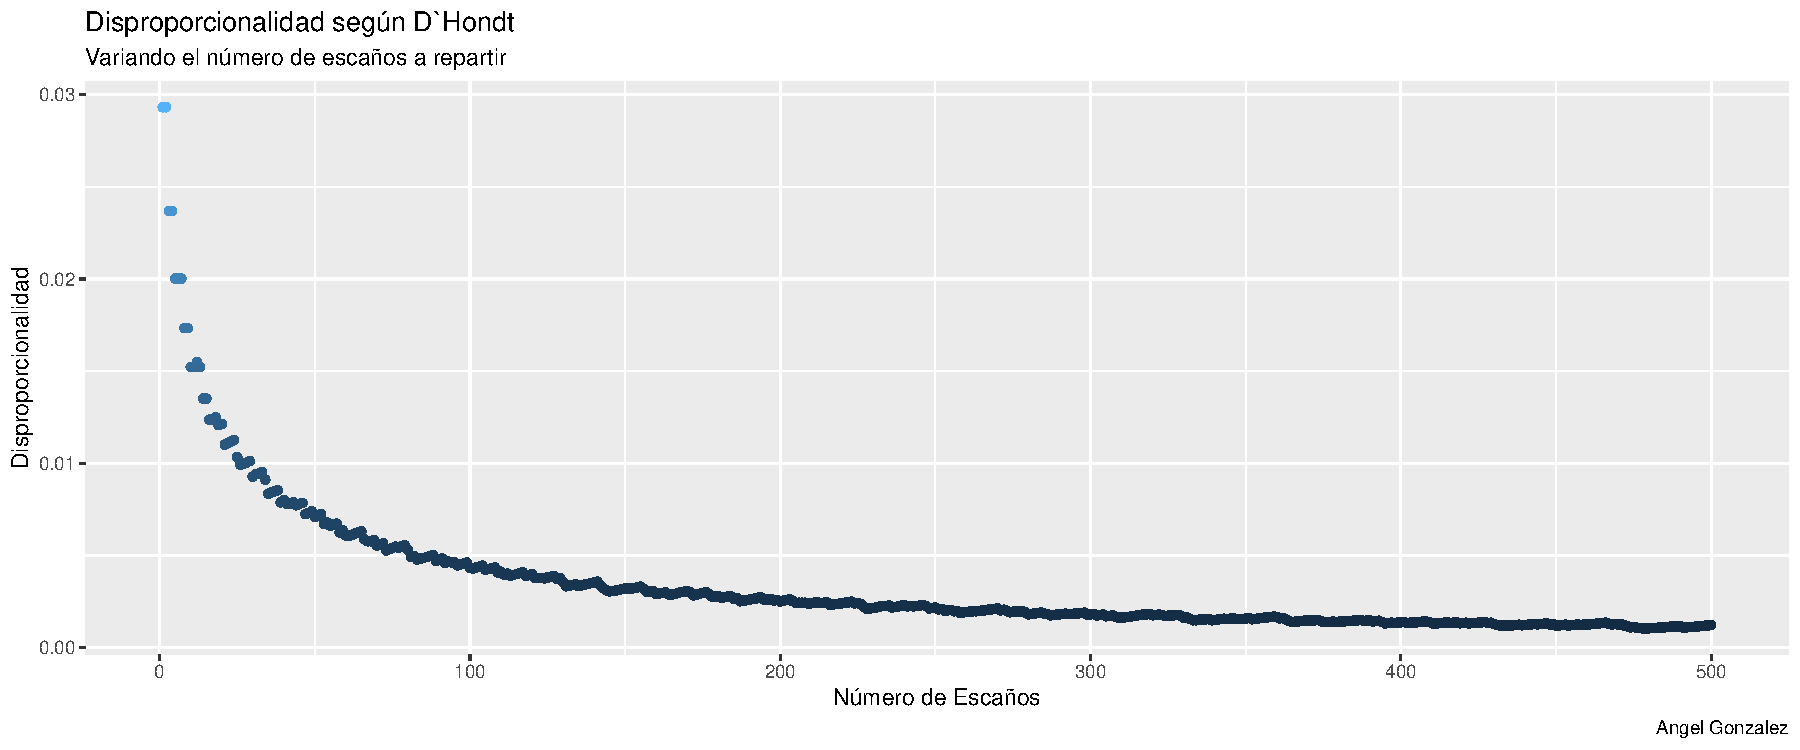
\includegraphics[width=0.95\linewidth]{figurasR/unnamed-chunk-9-1} \end{center}

En este caso se nos presenta la disproporcionalidad variando el número
de de escaños posibles, en el presente caso se empieza por repartir un
único escaño hasta los 500 posibles escaños. Observamos que la
disproporcionalidad en el caso de un escaño es muy alta, posteriormente
cuanto mayor es el número de escaños a repartir la disproporcionalidad
va bajando. La diferencia de disproporcionalidad en los casos en los que
hay pocos escaños a repartir es alta, cuantos mas escaños a repartir la
diferencia de disproporcionalidad entre sucesivos escaños va
reduciendose, a números altos de escaños a repartir la
disproporcionalidad tiende a estabilizarse.

\hypertarget{dhondt-variando-el-nuxfamero-de-partidos}{%
\subsubsection{D`Hondt variando el número de
partidos}\label{dhondt-variando-el-nuxfamero-de-partidos}}

\begin{center}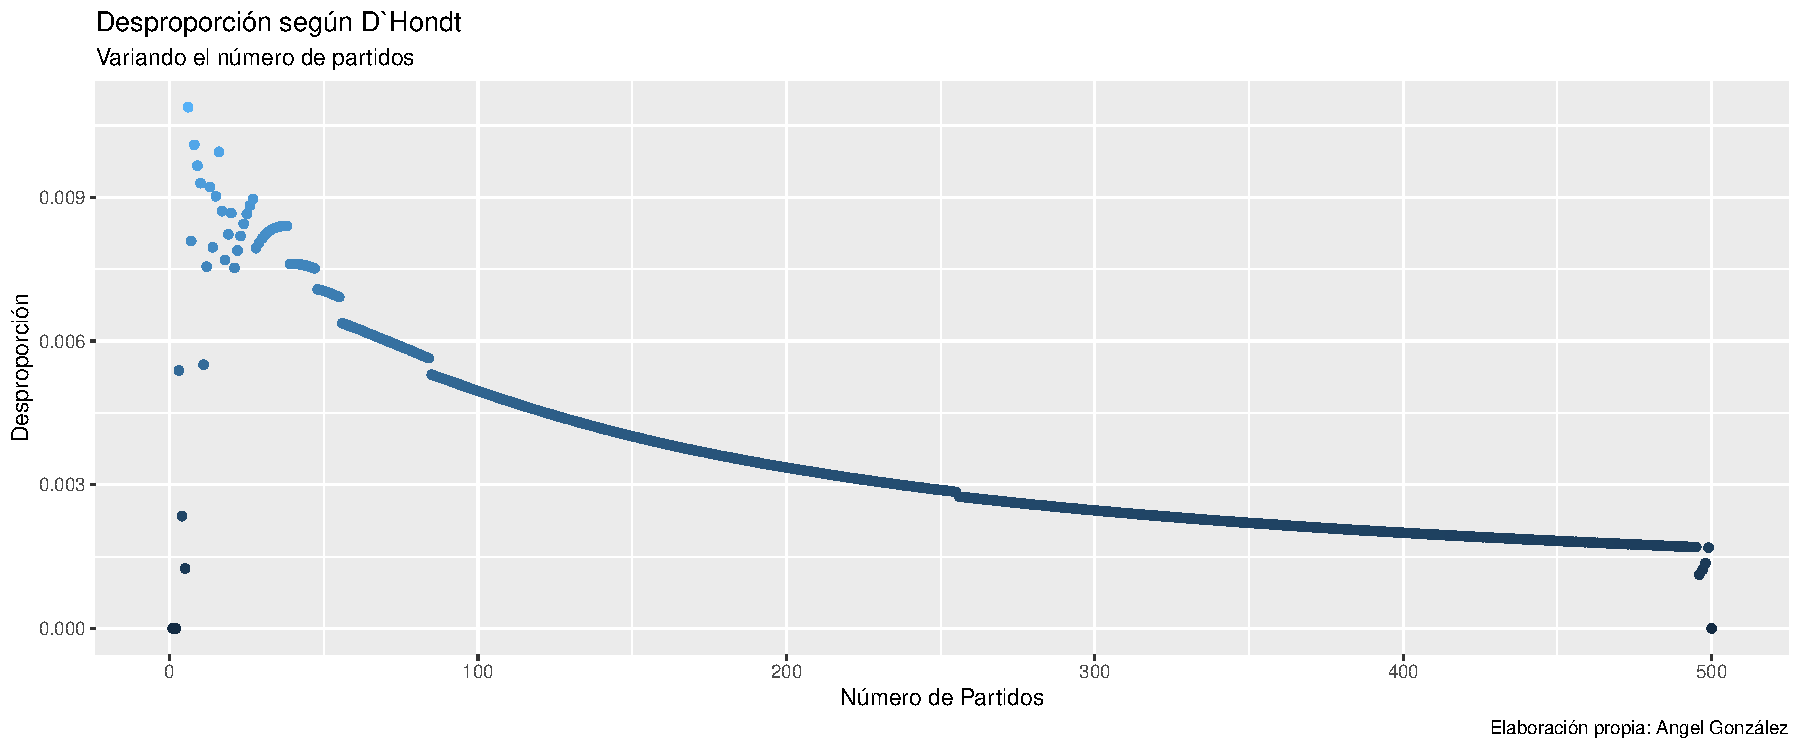
\includegraphics[width=0.95\linewidth]{figurasR/unnamed-chunk-10-1} \end{center}

En el caso presente únicamente modificamos el número de partidos
presentes en la elección, desde un único posible partido hasta 500
partidos que se presentan a una elección ficticia. Observamos que cuando
se presentan 2 o 3 partidos a las elecciones la disproporcionalidad es
baja, va aumentando a medida que se presentan más partidos, alcanzando
el máximo de disproporcionalidad con 6 partidos que se presentan a las
elecciones, a partir de el séptimo partido la curva comienza a decrecer.
Podemos apreciar en el gráfico que para un número bajo de partidos que
se presentan a las elecciones ( de 4 a 60 ) la disproporcionalidad es
alta pero decreciente, cuanto mayor número de partidos se presentan en
las elcciones menor es la disproporcionalidad que encontramos, como en
el apartado anterior, la disproporcionalidad tiende a estabilizarse.

\hypertarget{dhondt-variando-la-distribuciuxf3n-de-los-votos}{%
\subsubsection{D`Hondt variando la distribución de los
votos}\label{dhondt-variando-la-distribuciuxf3n-de-los-votos}}

\begin{center}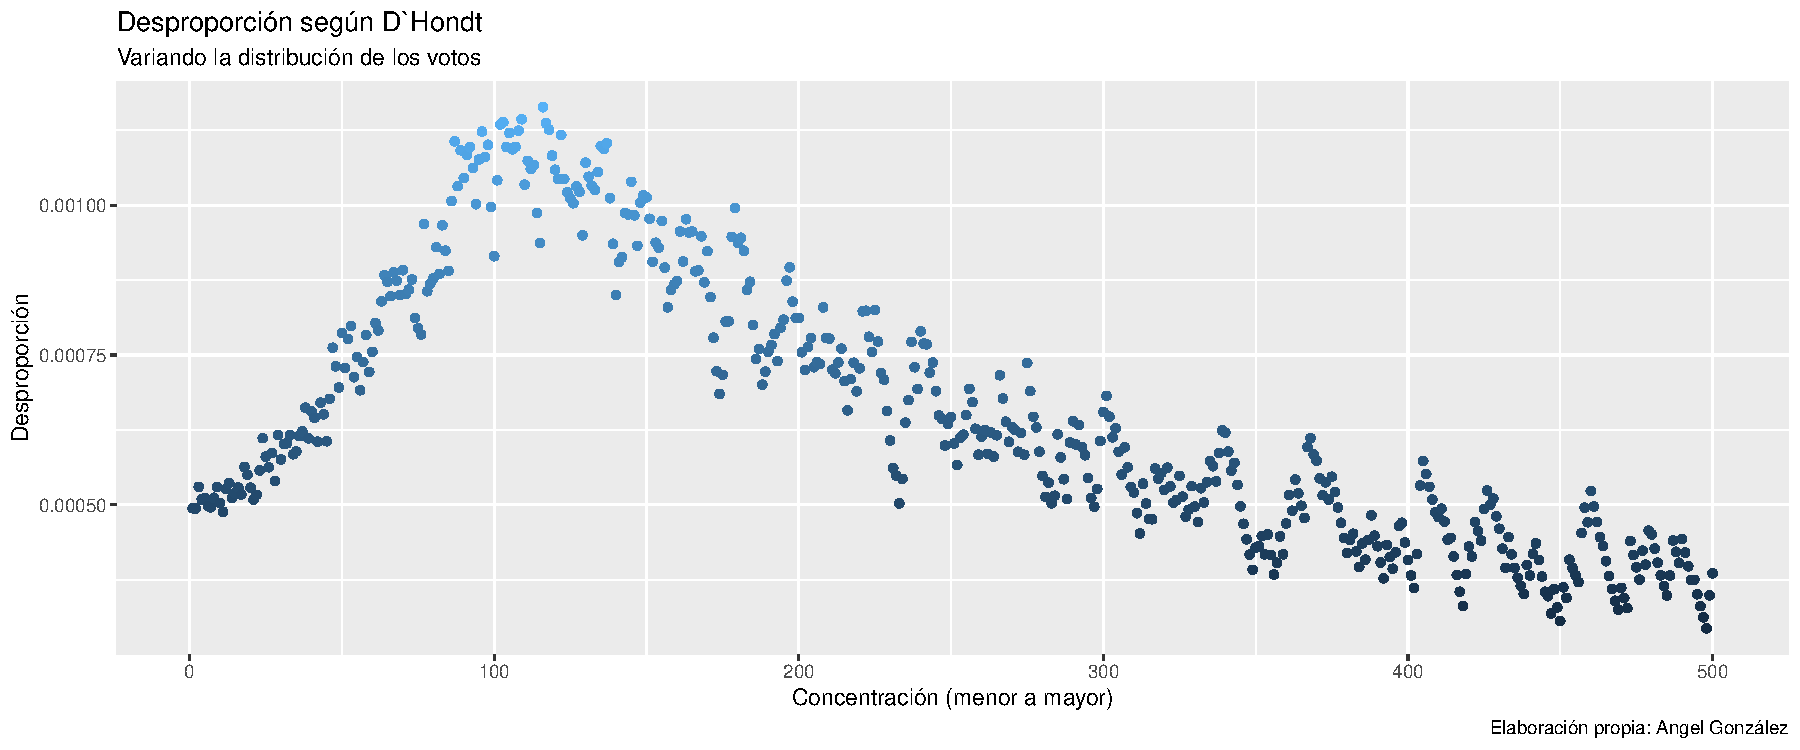
\includegraphics[width=0.95\linewidth]{figurasR/unnamed-chunk-11-1} \end{center}

En el presente gráfico variamos la distribución de los votos en unas
elecciones ficticias, comenzamos con una concentración de votos baja, es
decir, la diferencia de votos entre partidos es baja, hasta acabar con
una concentración de votos alta, en donde la diferencia de votos entre
partidos es muy grande. Observando el gráfico observamos que cuando la
concentración del voto es muy baja la disproporcionalidad está en un
nivel bajo, cuanto más concentración de voto podemos comprobar como la
disproporcionalidad aumenta hasta que alcanza un punto en donde alcanza
el máximo de disproporcionalidad y a partir de ese punto la
disproporcionalidad va bajando. Así podemos concluir que el reparto de
escaños según la ley D`Hondt es mejor cuanto más concentración de voto
tengan unos pocos partidos con respecto a los demás.

\hypertarget{sainte-lague}{%
\subsection{Sainte-Lague}\label{sainte-lague}}

\hypertarget{sainte-lague-variando-el-nuxfamero-de-escauxf1os}{%
\subsubsection{Sainte-Lague variando el número de
escaños}\label{sainte-lague-variando-el-nuxfamero-de-escauxf1os}}

\begin{verbatim}
## [1] 1.436887
\end{verbatim}

\begin{center}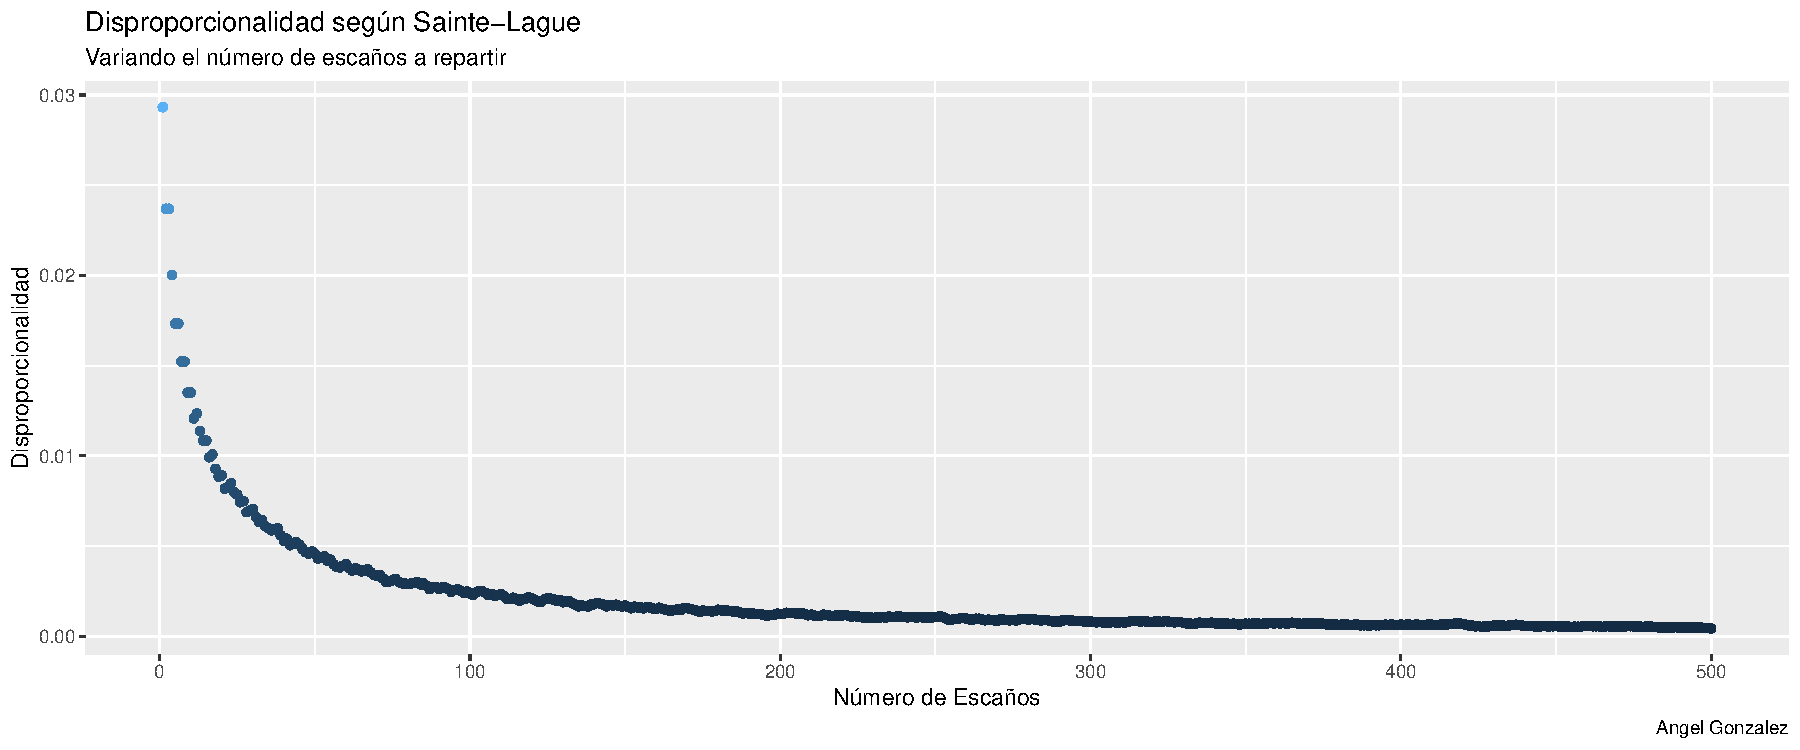
\includegraphics[width=0.95\linewidth]{figurasR/unnamed-chunk-14-1} \end{center}

En este caso se nos presenta la disproporcionalidad variando el número
de de escaños posibles, en el presente caso se empieza por repartir un
único escaño hasta los 500 posibles escaños. Observamos que la
disproporcionalidad en el caso de un escaño es muy alta, posteriormente
cuanto mayor es el número de escaños a repartir la disproporcionalidad
va bajando. La diferencia de disproporcionalidad en los casos en los que
hay pocos escaños a repartir es alta, cuantos mas escaños a repartir la
diferencia de disproporcionalidad entre sucesivos escaños va
reduciendose, a números altos de escaños a repartir la
disproporcionalidad tiende a estabilizarse.

\hypertarget{sainte-lague-variando-el-nuxfamero-de-partidos}{%
\subsubsection{Sainte-Lague variando el número de
partidos}\label{sainte-lague-variando-el-nuxfamero-de-partidos}}

\begin{center}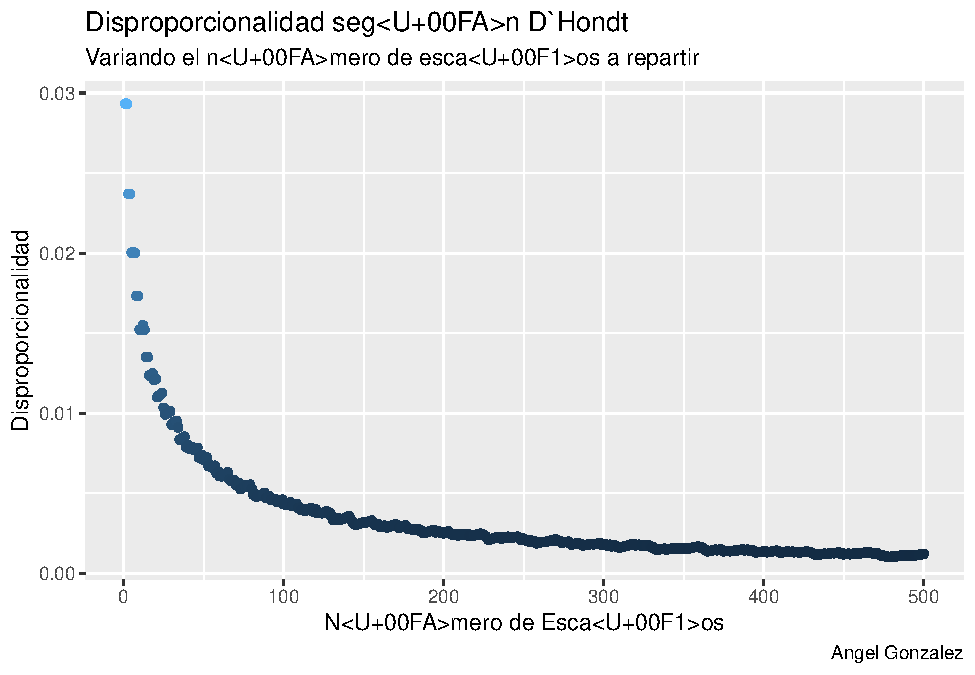
\includegraphics[width=0.95\linewidth]{figurasR/unnamed-chunk-15-1} \end{center}

En el caso presente únicamente modificamos el número de partidos
presentes en la elección, desde un único posible partido hasta 500
partidos que se presentan a una elección ficticia. Observamos que cuando
se presentan 2 partidos a las elecciones la disproporcionalidad es baja,
va aumentando a medida que se presentan más partidos, alcanzando el
máximo de disproporcionalidad con 2 partidos que se presentan a las
elecciones, a partir de el séptimo partido la curva comienza a decrecer.
Podemos apreciar en el gráfico que para un número bajo de partidos que
se presentan a las elecciones ( de 4 a 6 ) la disproporcionalidad es
alta pero decreciente, cuanto mayor número de partidos se presentan en
las elcciones menor es la disproporcionalidad que encontramos, como en
el apartado anterior, la disproporcionalidad tiende a estabilizarse.

\hypertarget{sainte-lague-variando-la-distribuciuxf3n-de-los-votos}{%
\subsubsection{Sainte-Lague variando la distribución de los
votos}\label{sainte-lague-variando-la-distribuciuxf3n-de-los-votos}}

\begin{center}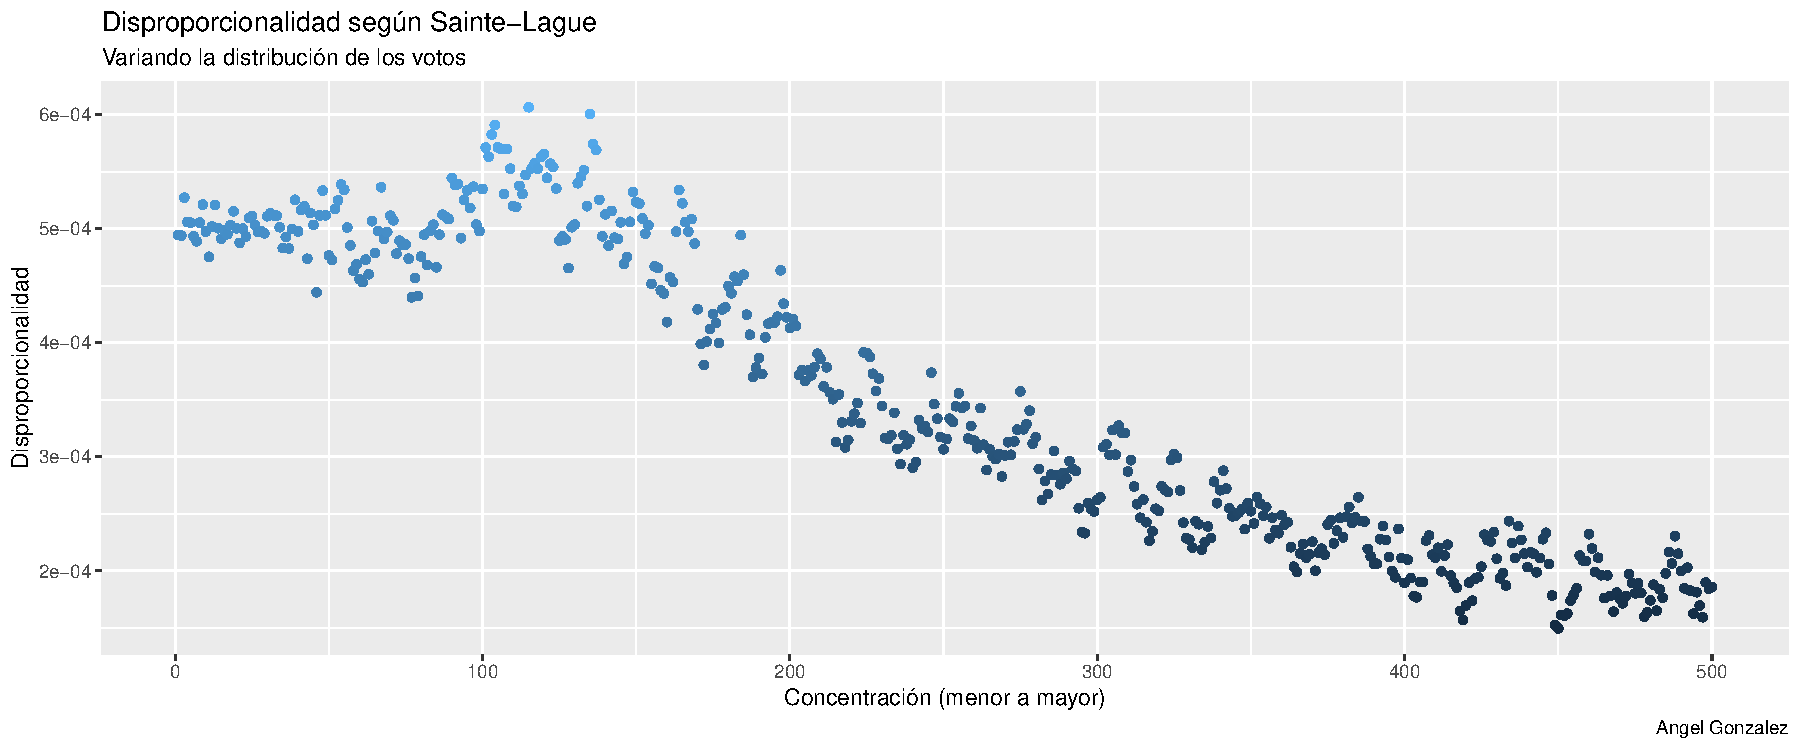
\includegraphics[width=0.95\linewidth]{figurasR/unnamed-chunk-16-1} \end{center}

En el presente gráfico variamos la distribución de los votos en unas
elecciones ficticias, comenzamos con una concentración de votos baja, es
decir, la diferencia de votos entre partidos es baja, hasta acabar con
una concentración de votos alta, en donde la diferencia de votos entre
partidos es muy grande. Observando el gráfico observamos que cuando la
concentración del voto es muy baja la disproporcionalidad está en un
nivel alto, aumenta levemente para una concentración baja-media y a
partir de ahí, donde alcanza el máximo de disproporcionalidad, la curva
va decreciendo cuanto mas diferencia de votos entre partidos exista. Así
podemos concluir que el reparto de escaños según la ley Sainte-Lague es
mejor cuanto más concentración de voto tengan unos pocos partidos con
respecto a los demás.

\hypertarget{modified-sainte-lague}{%
\subsection{Modified Sainte-Lague}\label{modified-sainte-lague}}

\hypertarget{modified-sainte-lague-variando-el-nuxfamero-de-escauxf1os}{%
\subsubsection{Modified Sainte-Lague variando el número de
escaños}\label{modified-sainte-lague-variando-el-nuxfamero-de-escauxf1os}}

\begin{verbatim}
## [1] 1.436887
\end{verbatim}

\begin{center}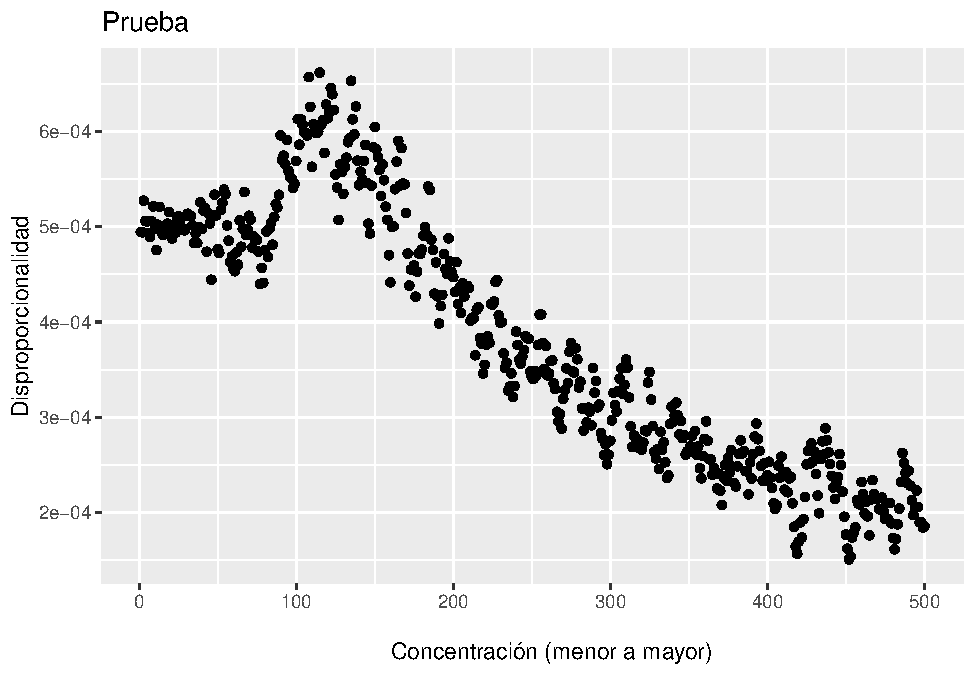
\includegraphics[width=0.95\linewidth]{figurasR/unnamed-chunk-19-1} \end{center}

En este caso se nos presenta la disproporcionalidad variando el número
de de escaños posibles, en el presente caso se empieza por repartir un
único escaño hasta los 500 posibles escaños. Observamos que la
disproporcionalidad en el caso de un escaño es muy alta, posteriormente
cuanto mayor es el número de escaños a repartir la disproporcionalidad
va bajando. La diferencia de disproporcionalidad en los casos en los que
hay pocos escaños a repartir es alta, cuantos mas escaños a repartir la
diferencia de disproporcionalidad entre sucesivos escaños va
reduciendose, a números altos de escaños a repartir la
disproporcionalidad tiende a estabilizarse.

\hypertarget{modified-sainte-lague-variando-el-nuxfamero-de-partidos}{%
\subsubsection{Modified Sainte-Lague variando el número de
partidos}\label{modified-sainte-lague-variando-el-nuxfamero-de-partidos}}

\begin{center}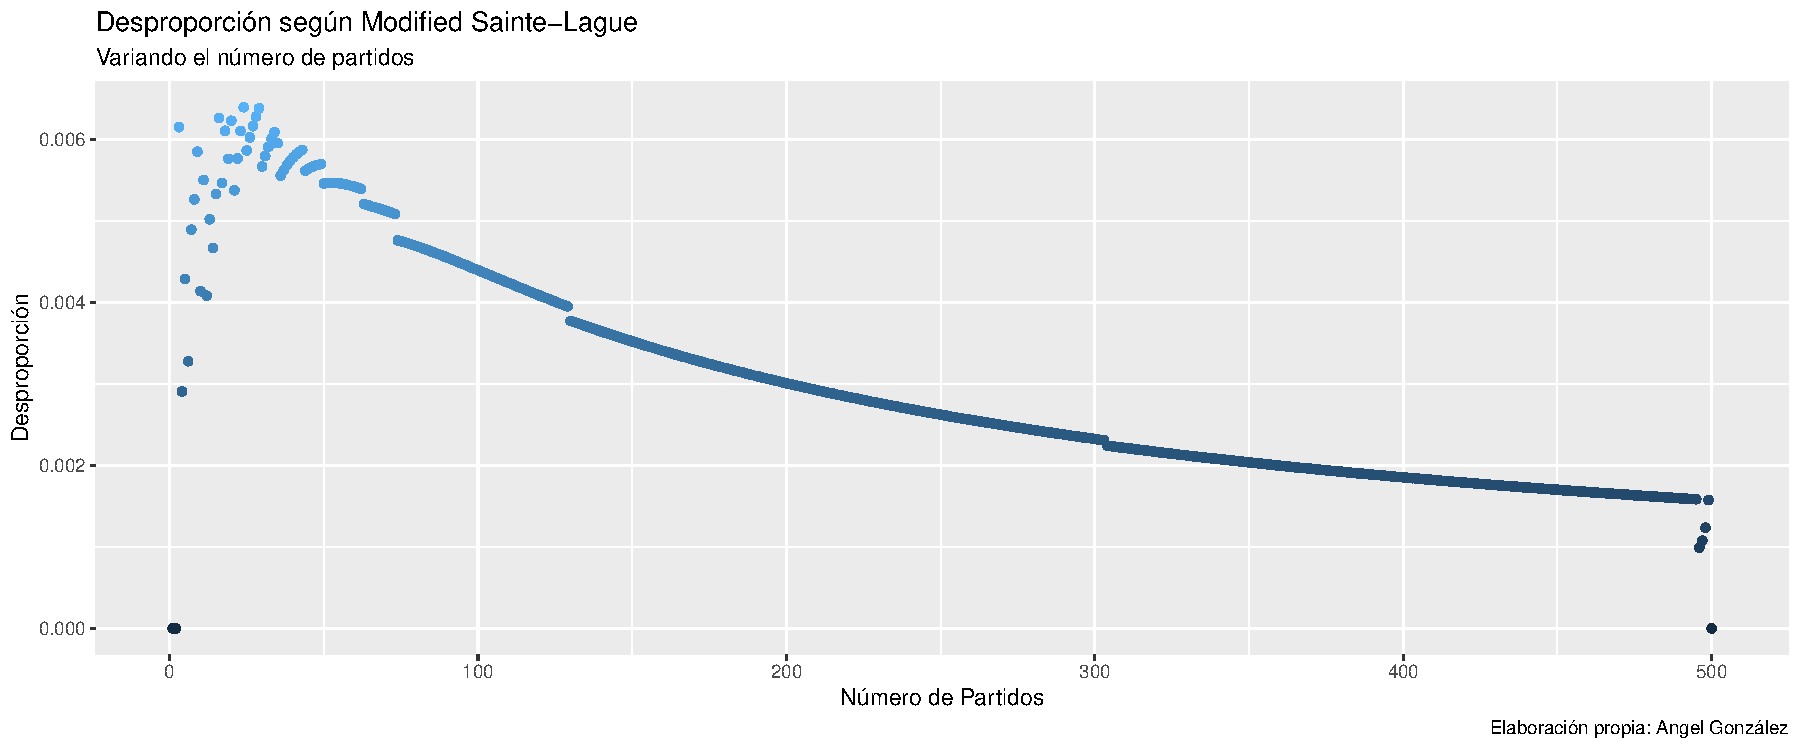
\includegraphics[width=0.95\linewidth]{figurasR/unnamed-chunk-20-1} \end{center}

En el caso presente únicamente modificamos el número de partidos
presentes en la elección, desde un único posible partido hasta 500
partidos que se presentan a una elección ficticia. Observamos que cuando
se presentan 2 o 3 partidos a las elecciones la disproporcionalidad es
baja, va aumentando a medida que se presentan más partidos, alcanzando
el máximo de disproporcionalidad con 6 partidos que se presentan a las
elecciones, a partir de el séptimo partido la curva comienza a decrecer.
Podemos apreciar en el gráfico que para un número bajo de partidos que
se presentan a las elecciones ( de 2 a 6 ) la disproporcionalidad es
alta pero decreciente, cuanto mayor número de partidos se presentan en
las elcciones menor es la disproporcionalidad que encontramos, como en
el apartado anterior, la disproporcionalidad tiende a estabilizarse.

\hypertarget{modified-sainte-lague-variando-la-distribuciuxf3n-de-los-votos}{%
\subsubsection{Modified Sainte-Lague variando la distribución de los
votos}\label{modified-sainte-lague-variando-la-distribuciuxf3n-de-los-votos}}

\begin{center}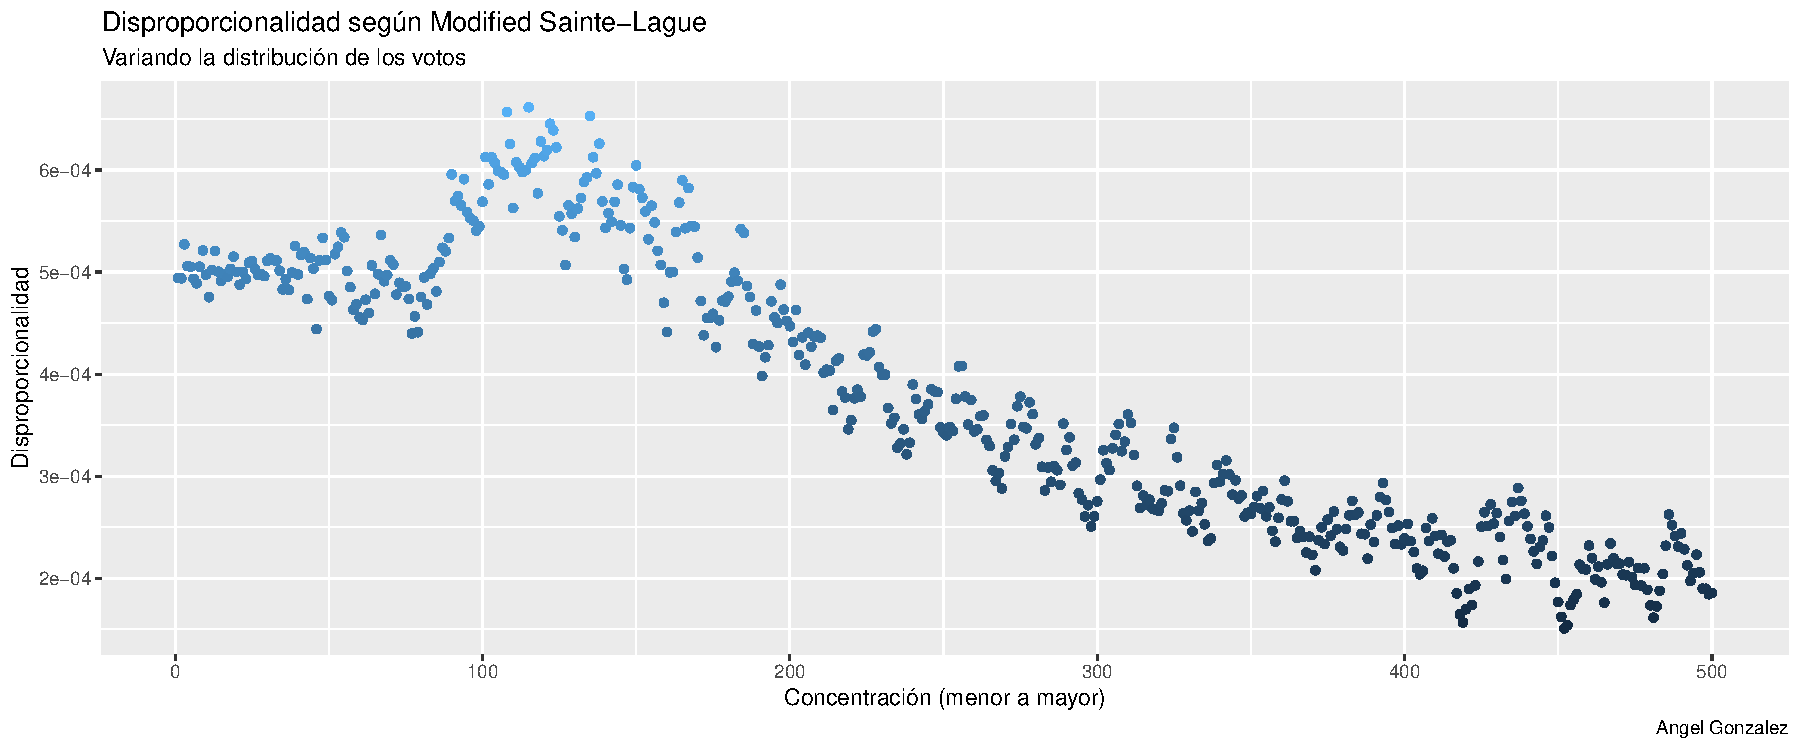
\includegraphics[width=0.95\linewidth]{figurasR/unnamed-chunk-21-1} \end{center}

En el presente gráfico variamos la distribución de los votos en unas
elecciones ficticias, comenzamos con una concentración de votos baja, es
decir, la diferencia de votos entre partidos es baja, hasta acabar con
una concentración de votos alta, en donde la diferencia de votos entre
partidos es muy grande. Observando el gráfico observamos que cuando la
concentración del voto es muy baja la disproporcionalidad está en un
nivel medio, cuanto más concentración de voto podemos comprobar como la
disproporcionalidad aumenta hasta que alcanza un punto en donde alcanza
el máximo de disproporcionalidad y a partir de ese punto la
disproporcionalidad va bajando. Así podemos concluir que el reparto de
escaños según la ley Modified Sainte-Lague es mejor cuanto más
concentración de voto tengan unos pocos partidos con respecto a los
demás.

\hypertarget{imperiali}{%
\subsection{Imperiali}\label{imperiali}}

\hypertarget{imperiali-variando-el-nuxfamero-de-escauxf1os}{%
\subsubsection{Imperiali variando el número de
escaños}\label{imperiali-variando-el-nuxfamero-de-escauxf1os}}

\begin{verbatim}
## [1] 1.436887
\end{verbatim}

\begin{center}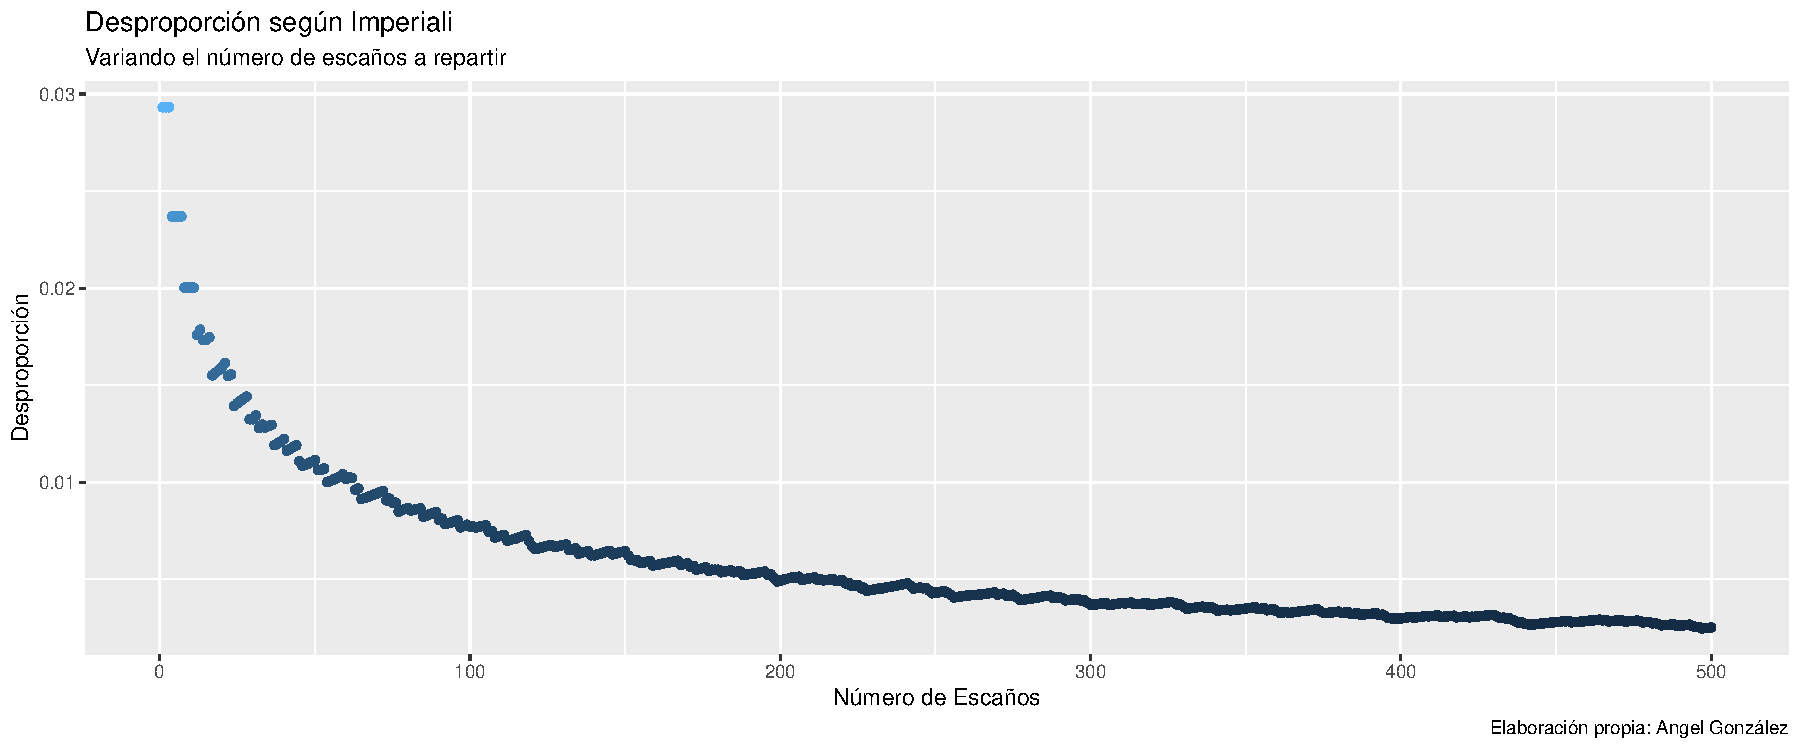
\includegraphics[width=0.95\linewidth]{figurasR/unnamed-chunk-24-1} \end{center}

En este caso se nos presenta la disproporcionalidad variando el número
de de escaños posibles, en el presente caso se empieza por repartir un
único escaño hasta los 500 posibles escaños. Observamos que la
disproporcionalidad en el caso de un escaño es muy alta, posteriormente
cuanto mayor es el número de escaños a repartir la disproporcionalidad
va bajando. La diferencia de disproporcionalidad en los casos en los que
hay pocos escaños a repartir es alta, cuantos mas escaños a repartir la
diferencia de disproporcionalidad entre sucesivos escaños va
reduciendose, a números altos de escaños a repartir la
disproporcionalidad tiende a estabilizarse.

\hypertarget{imperiali-variando-el-nuxfamero-de-partidos}{%
\subsubsection{Imperiali variando el número de
partidos}\label{imperiali-variando-el-nuxfamero-de-partidos}}

\begin{center}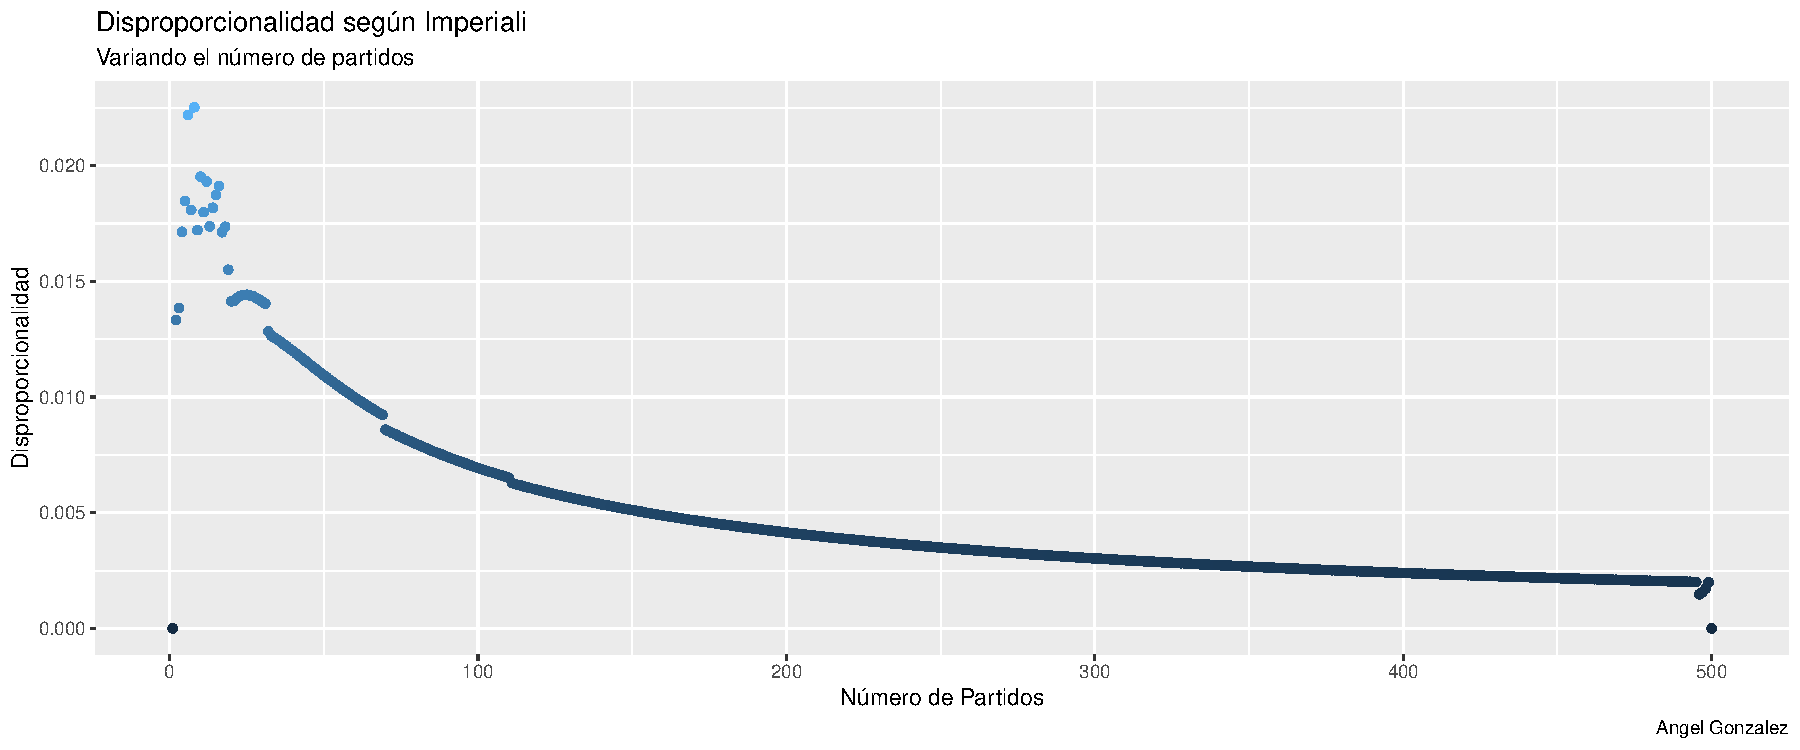
\includegraphics[width=0.95\linewidth]{figurasR/unnamed-chunk-25-1} \end{center}

En el caso presente únicamente modificamos el número de partidos
presentes en la elección, desde un único posible partido hasta 500
partidos que se presentan a una elección ficticia. Observamos que cuando
se presentan 2 o 3 partidos a las elecciones la disproporcionalidad es
baja, va aumentando a medida que se presentan más partidos, alcanzando
el máximo de disproporcionalidad con 6 partidos que se presentan a las
elecciones, a partir del séptimo partido la curva comienza a decrecer.
Entonces, según el modelo Imperiali tendremos una menor
disproporcionalidad según se vayan aumentando el número de partidos.

\hypertarget{imperiali-variando-la-distribuciuxf3n-de-los-votos}{%
\subsubsection{Imperiali variando la distribución de los
votos}\label{imperiali-variando-la-distribuciuxf3n-de-los-votos}}

\begin{center}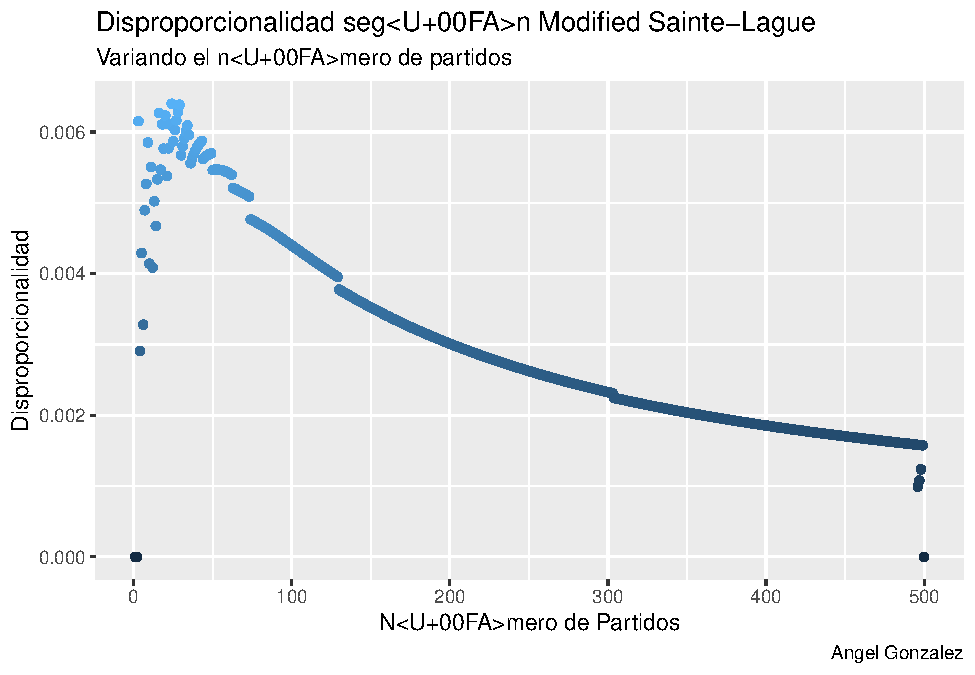
\includegraphics[width=0.95\linewidth]{figurasR/unnamed-chunk-26-1} \end{center}

En el presente gráfico variamos la distribución de los votos en unas
elecciones ficticias, comenzamos con una concentración de votos baja, es
decir, la diferencia de votos entre partidos es baja, hasta acabar con
una concentración de votos alta, en donde la diferencia de votos entre
partidos es muy grande. Observando el gráfico observamos que cuando la
concentración del voto es muy baja la disproporcionalidad está en un
nivel bajo, cuanto más concentración de voto podemos comprobar como la
disproporcionalidad aumenta hasta que alcanza un punto en donde alcanza
el máximo de disproporcionalidad y a partir de ese punto la
disproporcionalidad va bajando. Así podemos concluir que el reparto de
escaños según la ley Imperiali obtiene su menor disproporcionalidad en
los escenarios en donde la diferencia de votos entre los partidos sea
muy baja.

\hypertarget{huntington-hill}{%
\subsection{Huntington-Hill}\label{huntington-hill}}

\hypertarget{huntington-hill-variando-el-nuxfamero-de-escauxf1os}{%
\subsubsection{Huntington-Hill variando el número de
escaños}\label{huntington-hill-variando-el-nuxfamero-de-escauxf1os}}

\begin{verbatim}
## [1] 1.158221
\end{verbatim}

\begin{center}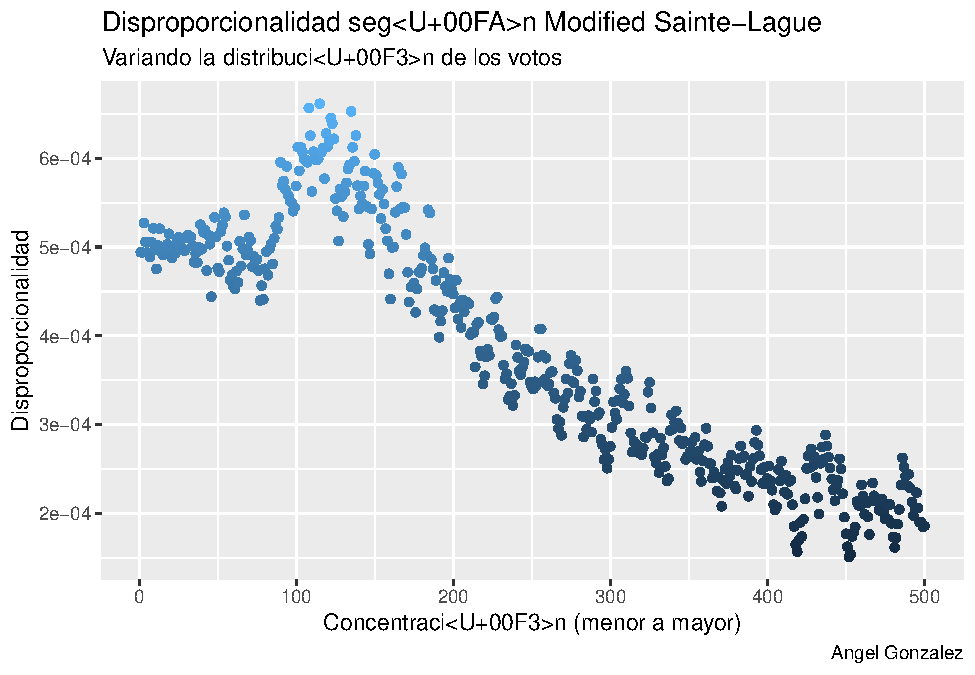
\includegraphics[width=0.95\linewidth]{figurasR/unnamed-chunk-29-1} \end{center}

En este caso se nos presenta la disproporcionalidad variando el número
de de escaños posibles, en el presente caso se empieza por repartir un
único escaño hasta los 500 posibles escaños. Observamos que la
disproporcionalidad en el caso de un escaño es muy alta,es interesante
observar que para un número de escaños entre 1 y 50 la
disproporcionalidad no cambia, es a partir de los 50 escaños y
posteriores donde observamos el descenso de la disproporcionalidad,
descenso rápido en los primeros escaños que tiende a estabilizarse
cuanto mayor número de escaños se repartan.

\hypertarget{huntington-hill-variando-el-nuxfamero-de-partidos}{%
\subsubsection{Huntington-Hill variando el número de
partidos}\label{huntington-hill-variando-el-nuxfamero-de-partidos}}

\begin{center}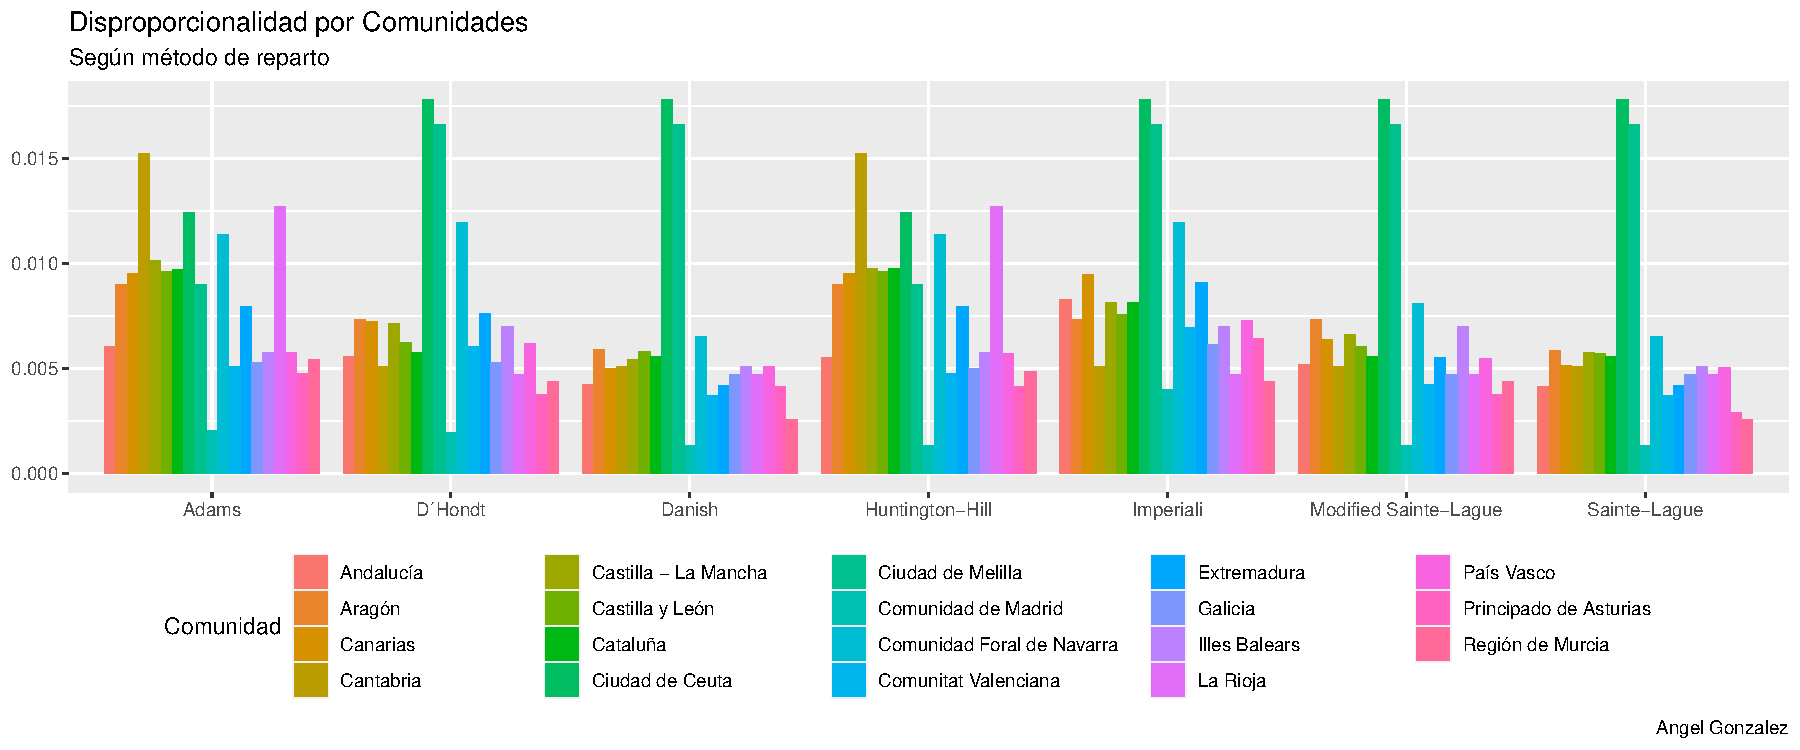
\includegraphics[width=0.95\linewidth]{figurasR/unnamed-chunk-30-1} \end{center}

En el caso presente únicamente modificamos el número de partidos
presentes en la elección, desde un único posible partido hasta 500
partidos que se presentan a una elección ficticia.

Observamos que cuando se presentan 2 o 3 partidos a las elecciones la
disproporcionalidad es media, va aumentando a medida que se presentan
más partidos, alcanzando el máximo de disproporcionalidad con 50
partidos que se presentan a las elecciones, a partir de 50 partidos la
curva comienza a decrecer.

Lo particular de este método respecto a otros métodos es que la menor
disproporcionalidad no se obtiene en el caso de que se presenten a las
elecciones pocos partidos, sino que la menor disproporcionalidad se
obtiene cuanto más partidos se presenten a las elecciones.

\hypertarget{huntington-hill-variando-la-distribuciuxf3n-de-los-votos}{%
\subsubsection{Huntington-Hill variando la distribución de los
votos}\label{huntington-hill-variando-la-distribuciuxf3n-de-los-votos}}

\begin{center}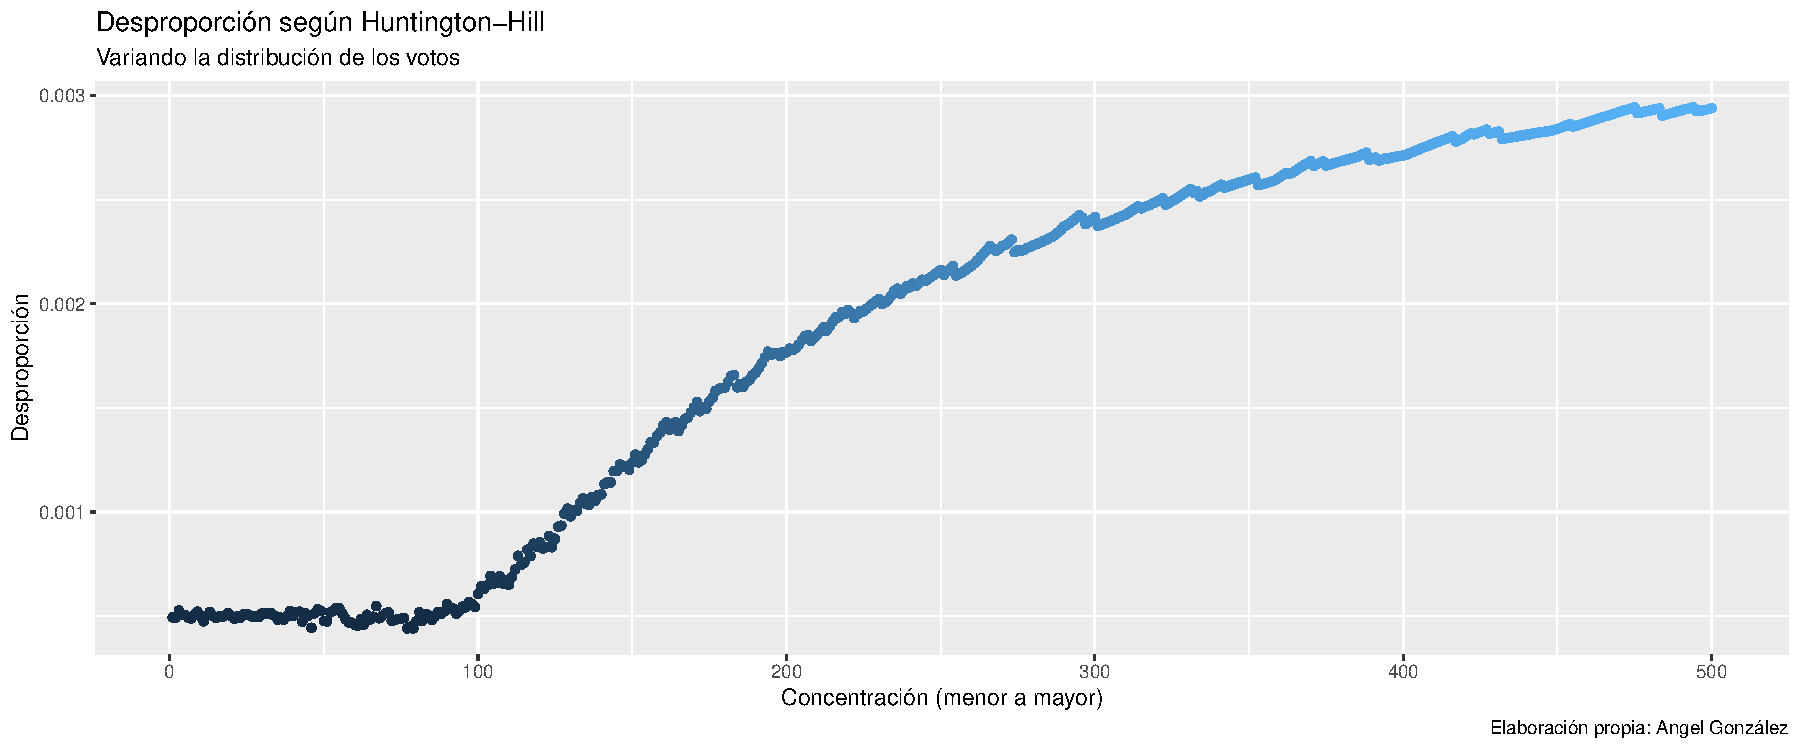
\includegraphics[width=0.95\linewidth]{figurasR/unnamed-chunk-31-1} \end{center}

En el presente gráfico variamos la distribución de los votos en unas
elecciones ficticias, comenzamos con una concentración de votos baja, es
decir, la diferencia de votos entre partidos es baja, hasta acabar con
una concentración de votos alta, en donde la diferencia de votos entre
partidos es muy grande.

Observando el gráfico observamos que cuando la concentración del voto es
muy baja la disproporcionalidad está en un nivel bajo,
disproporcionalidad que se mantiene baja cuando la concentración de los
votos es baja, y que a partir de una concentración de votos medio-baja
la disproporcionalidad va aumentando cuanto más diferencia de votos
entre partidos se presenten.

Así podemos concluir que el reparto de escaños según la ley
Huntington-Hill es mejor cuanto menor concentración de voto tengan los
partidos entre ellos, presenta un comportamiento diferente respecto a
los otros métodos en donde cuanto mayor concentración de votos menor
disproporcionalidad.

\hypertarget{adams}{%
\subsection{Adams}\label{adams}}

\hypertarget{adams-variando-el-nuxfamero-de-escauxf1os}{%
\subsubsection{Adams variando el número de
escaños}\label{adams-variando-el-nuxfamero-de-escauxf1os}}

\begin{verbatim}
## [1] 1.158221
\end{verbatim}

\begin{center}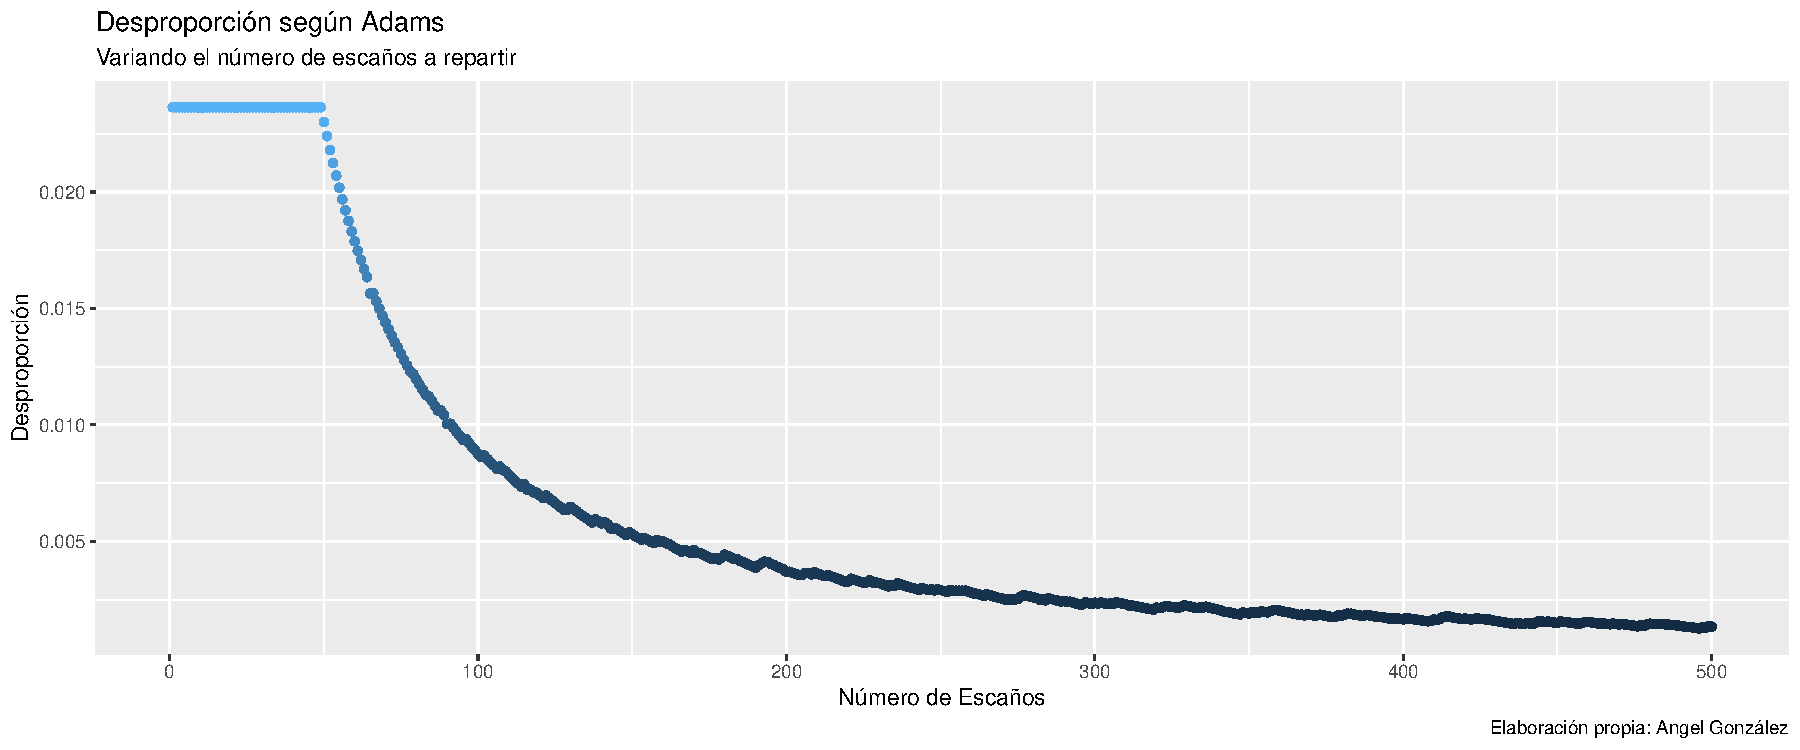
\includegraphics[width=0.95\linewidth]{figurasR/unnamed-chunk-34-1} \end{center}

En este caso se nos presenta la disproporcionalidad variando el número
de de escaños posibles, en el presente caso se empieza por repartir un
único escaño hasta los 500 posibles escaños. Observamos que la
disproporcionalidad en el caso de un escaño es muy alta, en este método
también observamos que la disproporcionalidad se mantiene en un mismo
nivel hasta los 50 escaños, posteriormente cuanto mayor es el número de
escaños a repartir la disproporcionalidad va bajando. La diferencia de
disproporcionalidad en los casos en los que hay pocos escaños a repartir
es alta, cuantos mas escaños a repartir la diferencia de
disproporcionalidad entre sucesivos escaños va reduciendose, a números
altos de escaños a repartir la disproporcionalidad tiende a
estabilizarse.

\hypertarget{adams-variando-el-nuxfamero-de-partidos}{%
\subsubsection{Adams variando el número de
partidos}\label{adams-variando-el-nuxfamero-de-partidos}}

\begin{center}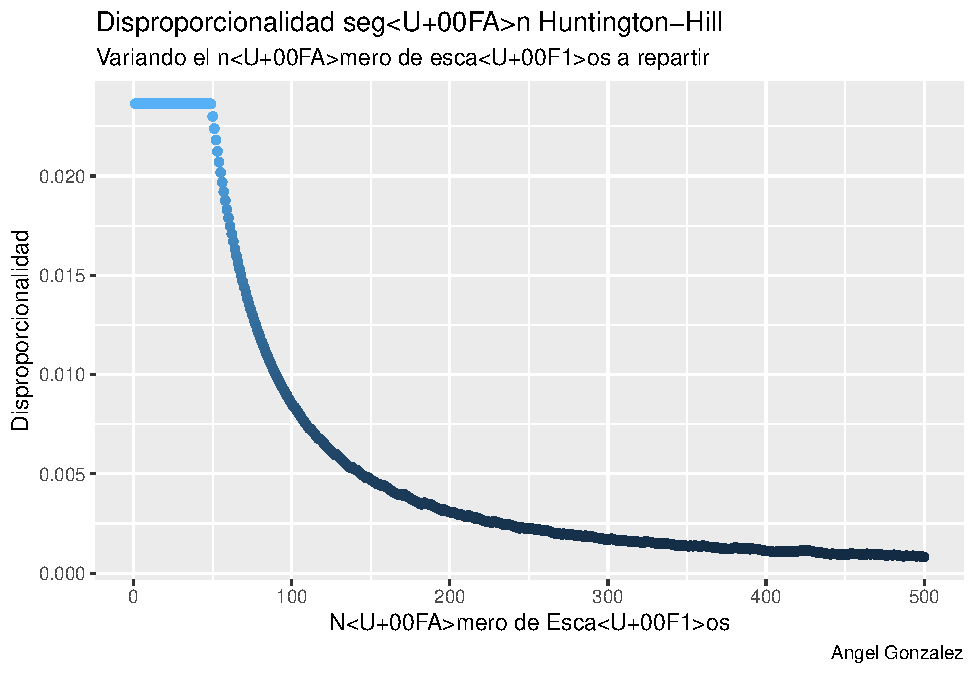
\includegraphics[width=0.95\linewidth]{figurasR/unnamed-chunk-35-1} \end{center}

En el caso presente únicamente modificamos el número de partidos
presentes en la elección, desde un único posible partido hasta 500
partidos que se presentan a una elección ficticia.

Observamos que cuando se presentan 2 o 3 partidos a las elecciones la
disproporcionalidad es media, va aumentando a medida que se presentan
más partidos, alcanzando el máximo de disproporcionalidad con 50
partidos que se presentan a las elecciones, a partir de los 50 partidos
que se presentan a las elecciones la curva comienza a decrecer.

Entonces según el método Adams obtenemos el mejor resultado cuanto mayor
número de partidos se presenten a las elecciones.

\hypertarget{adams-variando-la-distribuciuxf3n-de-los-votos}{%
\subsubsection{Adams variando la distribución de los
votos}\label{adams-variando-la-distribuciuxf3n-de-los-votos}}

\begin{center}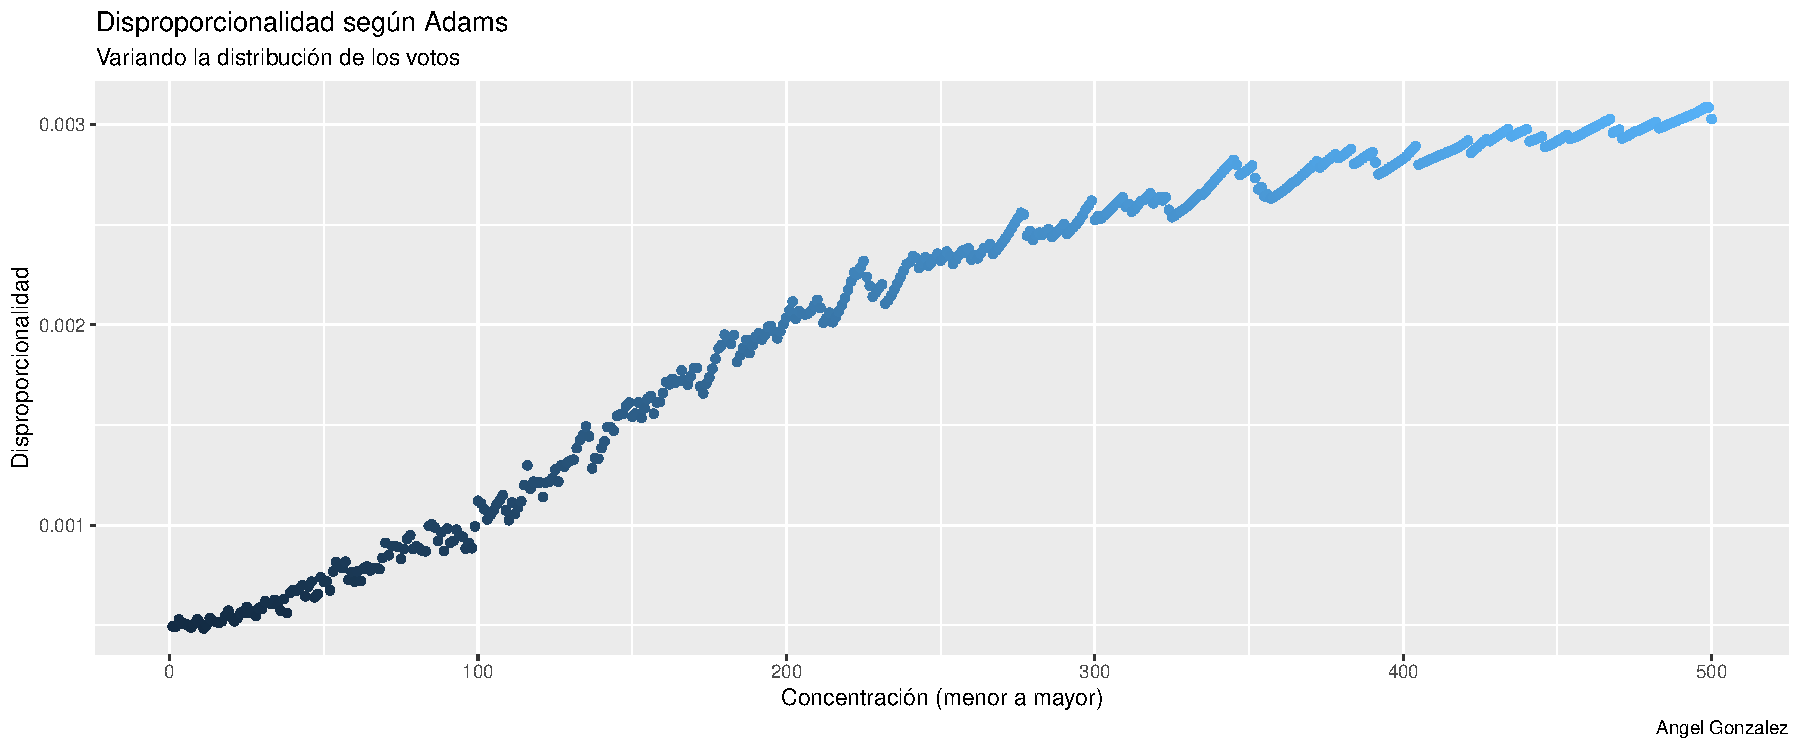
\includegraphics[width=0.95\linewidth]{figurasR/unnamed-chunk-36-1} \end{center}

En el presente gráfico variamos la distribución de los votos en unas
elecciones ficticias, comenzamos con una concentración de votos baja, es
decir, la diferencia de votos entre partidos es baja, hasta acabar con
una concentración de votos alta, en donde la diferencia de votos entre
partidos es muy grande.

Observando el gráfico observamos que cuando la concentración del voto es
muy baja la disproporcionalidad está en un nivel bajo, cuanto más
concentración de voto podemos comprobar como la disproporcionalidad va
aumentando cada vez con una diferencia decreciente.

Así podemos concluir que el reparto de escaños según la ley Adams es
mejor cuanto menor concentración de voto los partidos entre ellos, y
será peor cuanto mayor concentración de voto se presente.

\hypertarget{danish}{%
\subsection{Danish}\label{danish}}

\hypertarget{danish-variando-el-nuxfamero-de-escauxf1os}{%
\subsubsection{Danish variando el número de
escaños}\label{danish-variando-el-nuxfamero-de-escauxf1os}}

\begin{verbatim}
## [1] 1.436887
\end{verbatim}

\begin{center}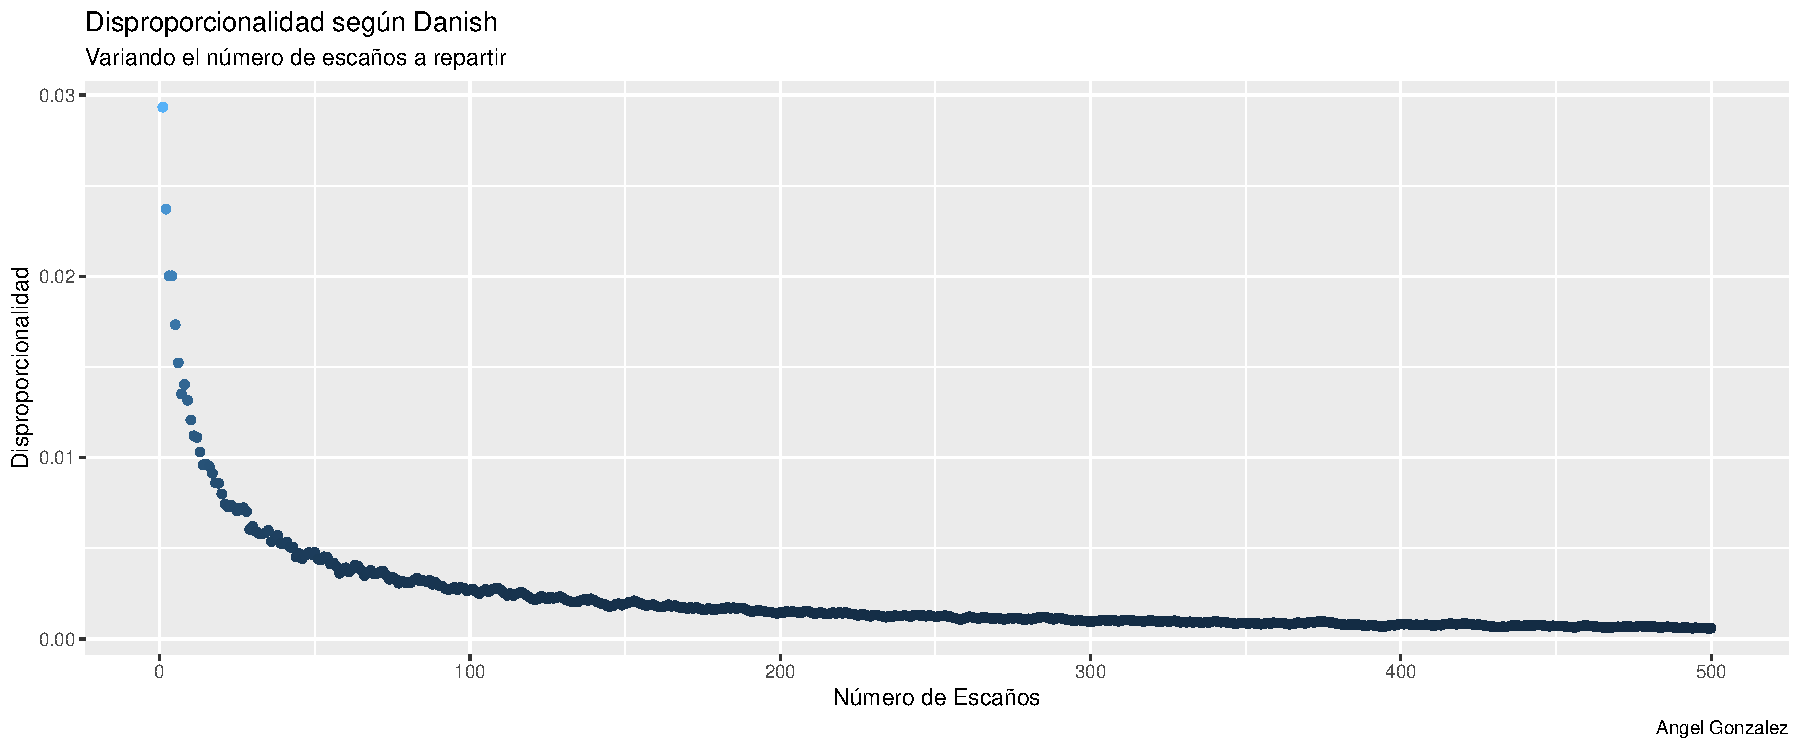
\includegraphics[width=0.95\linewidth]{figurasR/unnamed-chunk-39-1} \end{center}

En este caso se nos presenta la disproporcionalidad variando el número
de de escaños posibles, en el presente caso se empieza por repartir un
único escaño hasta los 500 posibles escaños. Observamos que la
disproporcionalidad en el caso de un escaño es muy alta, posteriormente
cuanto mayor es el número de escaños a repartir la disproporcionalidad
va bajando. La diferencia de disproporcionalidad en los casos en los que
hay pocos escaños a repartir es alta, cuantos mas escaños a repartir la
diferencia de disproporcionalidad entre sucesivos escaños va
reduciendose, a números altos de escaños a repartir la
disproporcionalidad tiende a estabilizarse.

\hypertarget{danish-variando-el-nuxfamero-de-partidos}{%
\subsubsection{Danish variando el número de
partidos}\label{danish-variando-el-nuxfamero-de-partidos}}

\begin{center}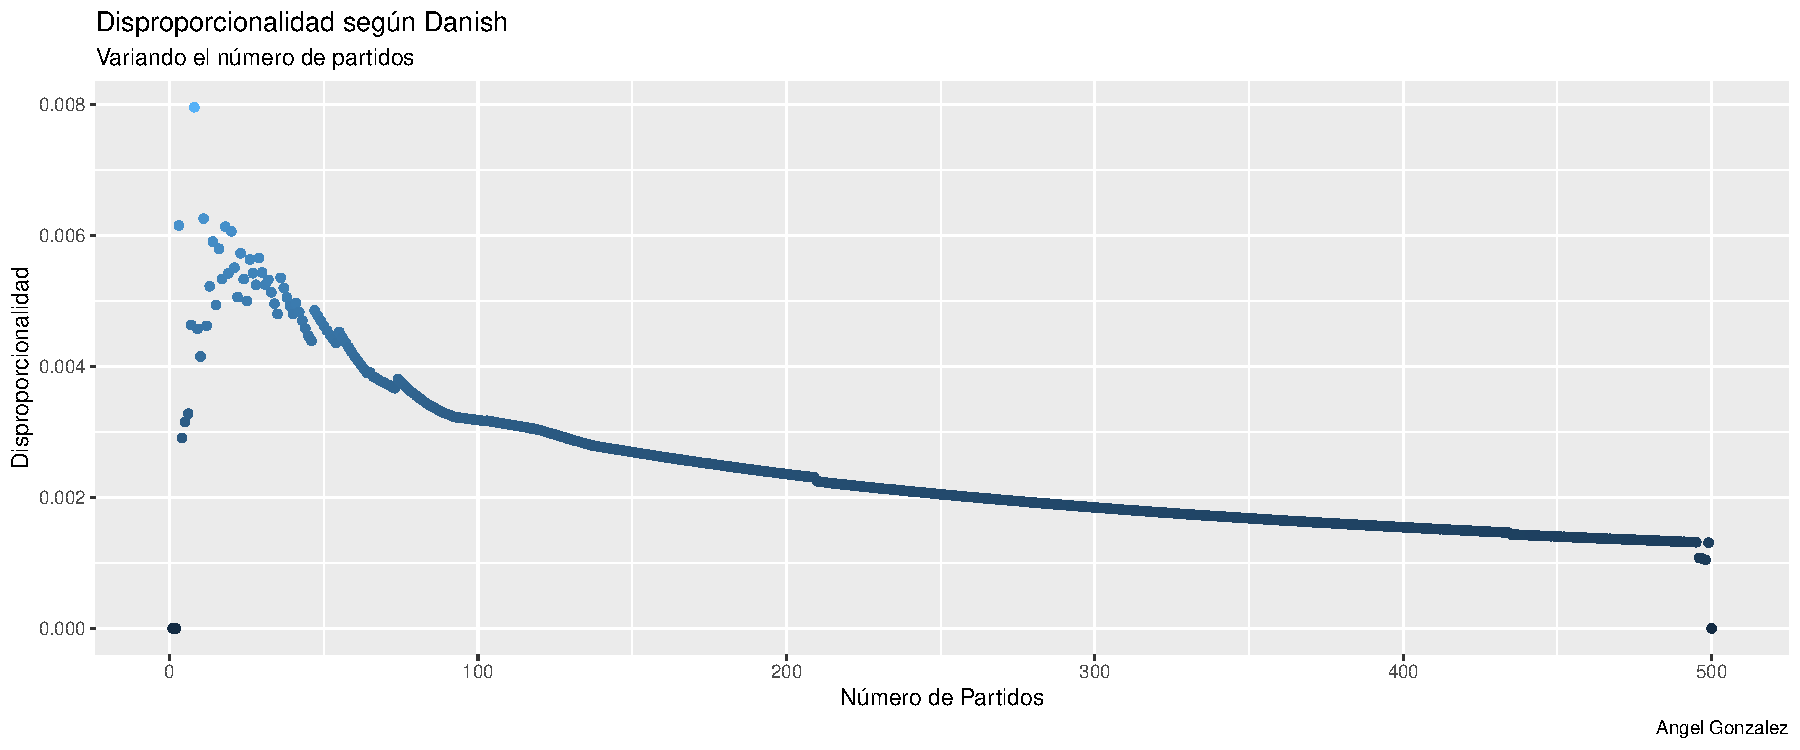
\includegraphics[width=0.95\linewidth]{figurasR/unnamed-chunk-40-1} \end{center}

En el caso presente únicamente modificamos el número de partidos
presentes en la elección, desde un único posible partido hasta 500
partidos que se presentan a una elección ficticia. Observamos que cuando
se presentan 2 o 3 partidos a las elecciones la disproporcionalidad es
baja, va aumentando a medida que se presentan más partidos, alcanzando
el máximo de disproporcionalidad con 6 partidos que se presentan a las
elecciones, a partir de el séptimo partido la curva comienza a decrecer.
Podemos apreciar en el gráfico que para un número bajo de partidos que
se presentan a las elecciones ( de 4 a 6 ) la disproporcionalidad es
alta pero decreciente, cuanto mayor número de partidos se presentan en
las elecciones menor es la disproporcionalidad que encontramos, como en
el apartado anterior, la disproporcionalidad tiende a estabilizarse.

Entonces según el método Danish obtenemos el mejor resultado cuanto más
partidos se presenten a las elecciones.

\hypertarget{danish-variando-la-distribuciuxf3n-de-los-votos}{%
\subsubsection{Danish variando la distribución de los
votos}\label{danish-variando-la-distribuciuxf3n-de-los-votos}}

\begin{center}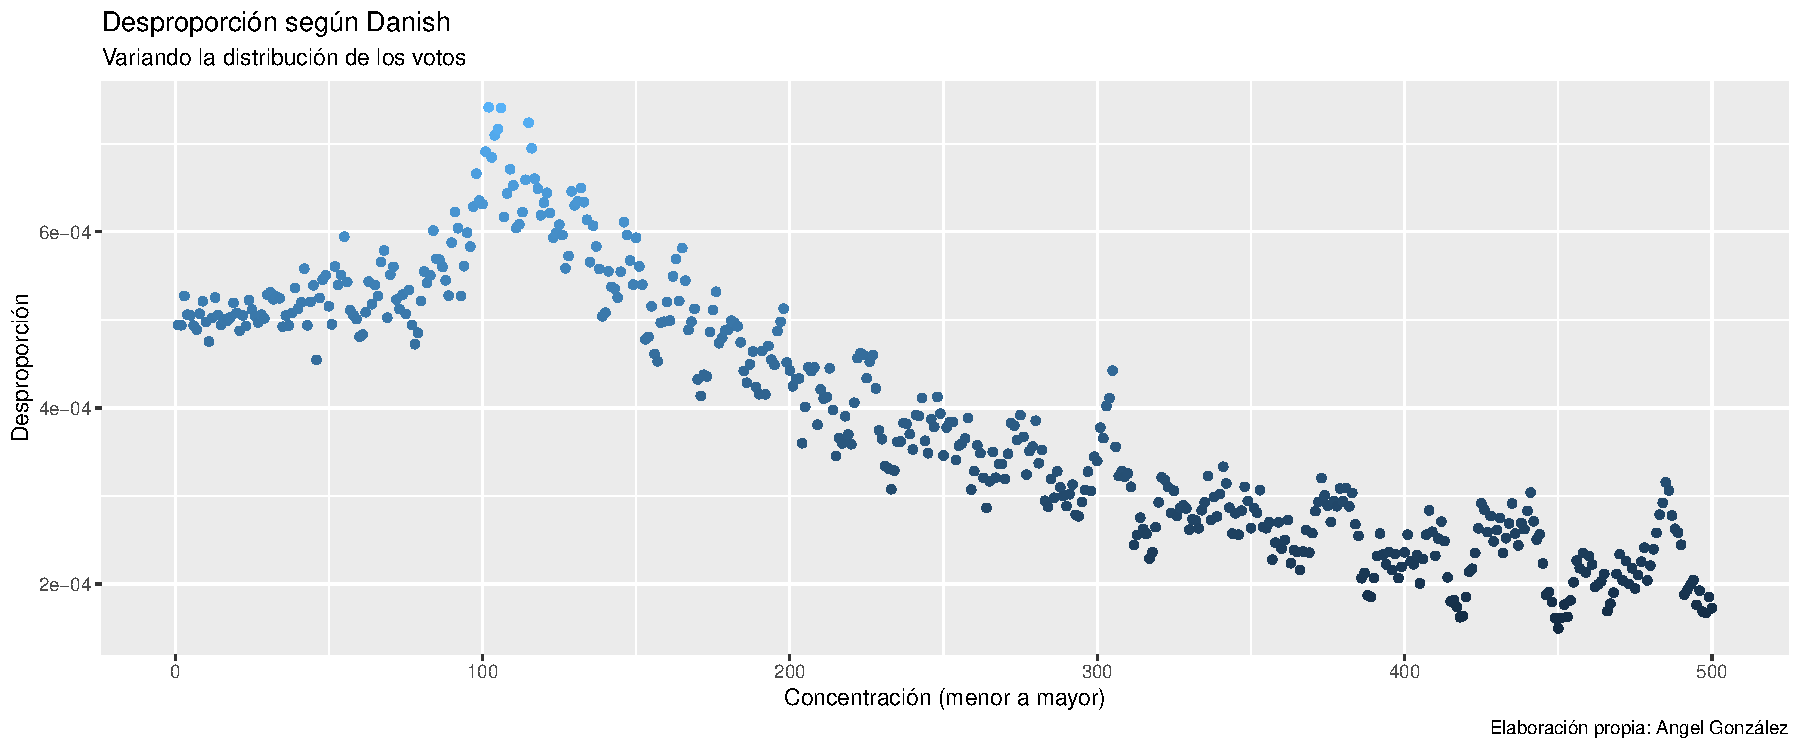
\includegraphics[width=0.95\linewidth]{figurasR/unnamed-chunk-41-1} \end{center}

En el presente gráfico variamos la distribución de los votos en unas
elecciones ficticias, comenzamos con una concentración de votos baja, es
decir, la diferencia de votos entre partidos es baja, hasta acabar con
una concentración de votos alta, en donde la diferencia de votos entre
partidos es muy grande.

Observando el gráfico observamos que cuando la concentración del voto es
muy baja la disproporcionalidad está en un nivel medio, cuanto más
concentración de voto podemos comprobar como la disproporcionalidad
aumenta hasta que alcanza un punto en donde alcanza el máximo de
disproporcionalidad y a partir de ese punto la disproporcionalidad va
bajando.

Así podemos concluir que el reparto de escaños según la ley Danish es
mejor cuanto más concentración de voto tengan unos pocos partidos con
respecto a los demás.

\hypertarget{comparaciones-entre-muxe9todos}{%
\section{Comparaciones entre
métodos}\label{comparaciones-entre-muxe9todos}}

\hypertarget{variando-el-nuxfamero-de-escauxf1os}{%
\subsection{Variando el número de
escaños}\label{variando-el-nuxfamero-de-escauxf1os}}

\begin{center}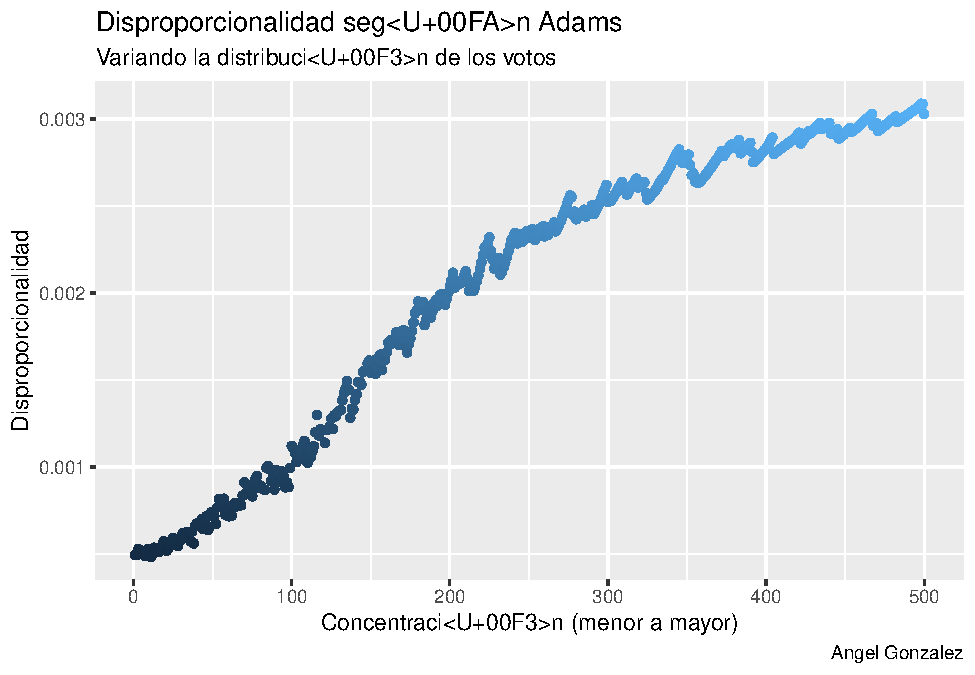
\includegraphics[width=0.95\linewidth]{figurasR/unnamed-chunk-42-1} \end{center}

En el presente gráfico comparamos en un mismo lugar los métodos
anteriormente analizados individualmente. En esta comparación podemos
observar que para todos los métodos la disproporcionalidad baja cuanto
mayor número de escaños a repartir, los peores métodos en este caso
serían el Adams y el Imperiali, el método Adams cuando tengamos un
número de escaños menor y el Imperiali a partir aproximadamente de los
100 escaños. Los mejores métodos en este caso serían el método de
Sainte-Lague y el método Danish.

\begin{center}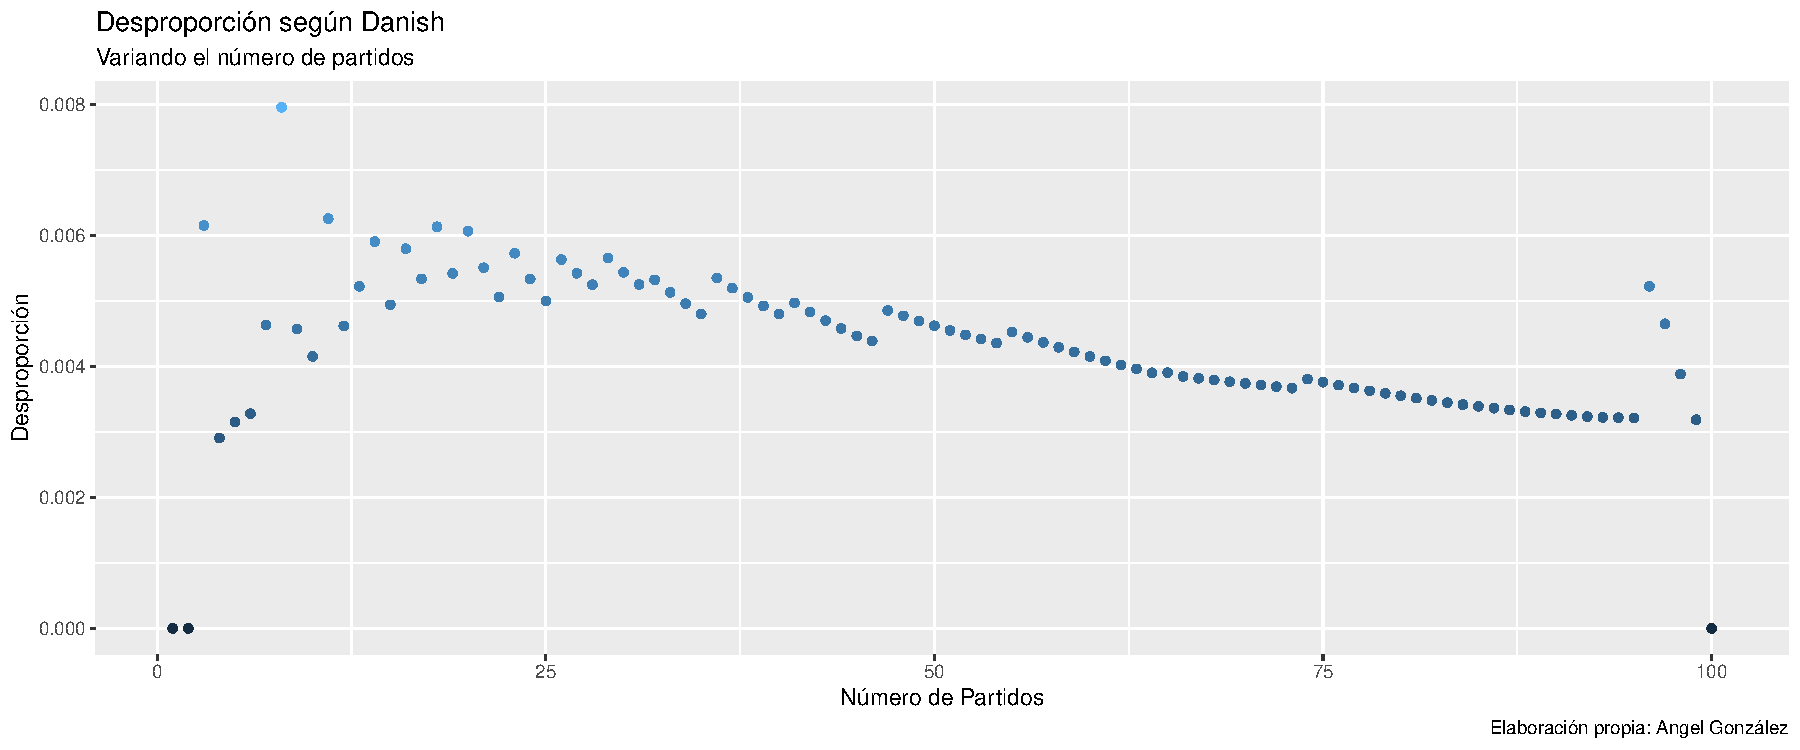
\includegraphics[width=0.95\linewidth]{figurasR/unnamed-chunk-43-1} \end{center}

En este gráfico nos centramos en la disproporcionalidad para un número
de escaños a repartir de entre 300 y 400 diputados, actualmente en
España se reparten 350 diputados. El peor método entre los presentados
es el método Imperiali, con una diferencia significatica respecto a los
demás métodos. Los mejores métodos de reparto podemos agruparlos en un
grupo de tres, que son el método de Sainte-Lague en primer lugar, el
método Modified Sainte-Lague y el método Danish respectivamente. Podemos
agrupar los métodos en tres grupos,un grupo que sería el de una
disproporcionalidad baja, en el que se encontrarían los métodos de
Sainte-Lague, Danish y Modified Sainte-Lague. Un segundo grupo que sería
el que presentaría una disproporcionalidad media, con los métodos Adams,
Huntington-Hill y D´Hondt, finalizando con un último grupo de
disproporcionalidad alta, y debido a ello no deseable en el que estaría
el método Imperiali.

Actualmente en España se reparten 350 escaños y se utiliza el método
D´Hondt, según los datos obtenidos podemos decir que no es el mejor
método que se puede utilizar, es un método que está en el grupo de
dispropocionalidad media, e incluso no es el mejor método dentro de ese
subgrupo, sería interesante según lo observado en la gráfica plantearse
un cambio de método a otro mejor, al menos a alguno dentro del subgrupo
de disproporcionalidad baja, preferentemente el mejor método que
podríamos utilizar, que sería el método de Sainte-Lague sin modificar.

\hypertarget{variando-el-nuxfamero-de-partidos}{%
\subsection{Variando el número de
partidos}\label{variando-el-nuxfamero-de-partidos}}

\begin{center}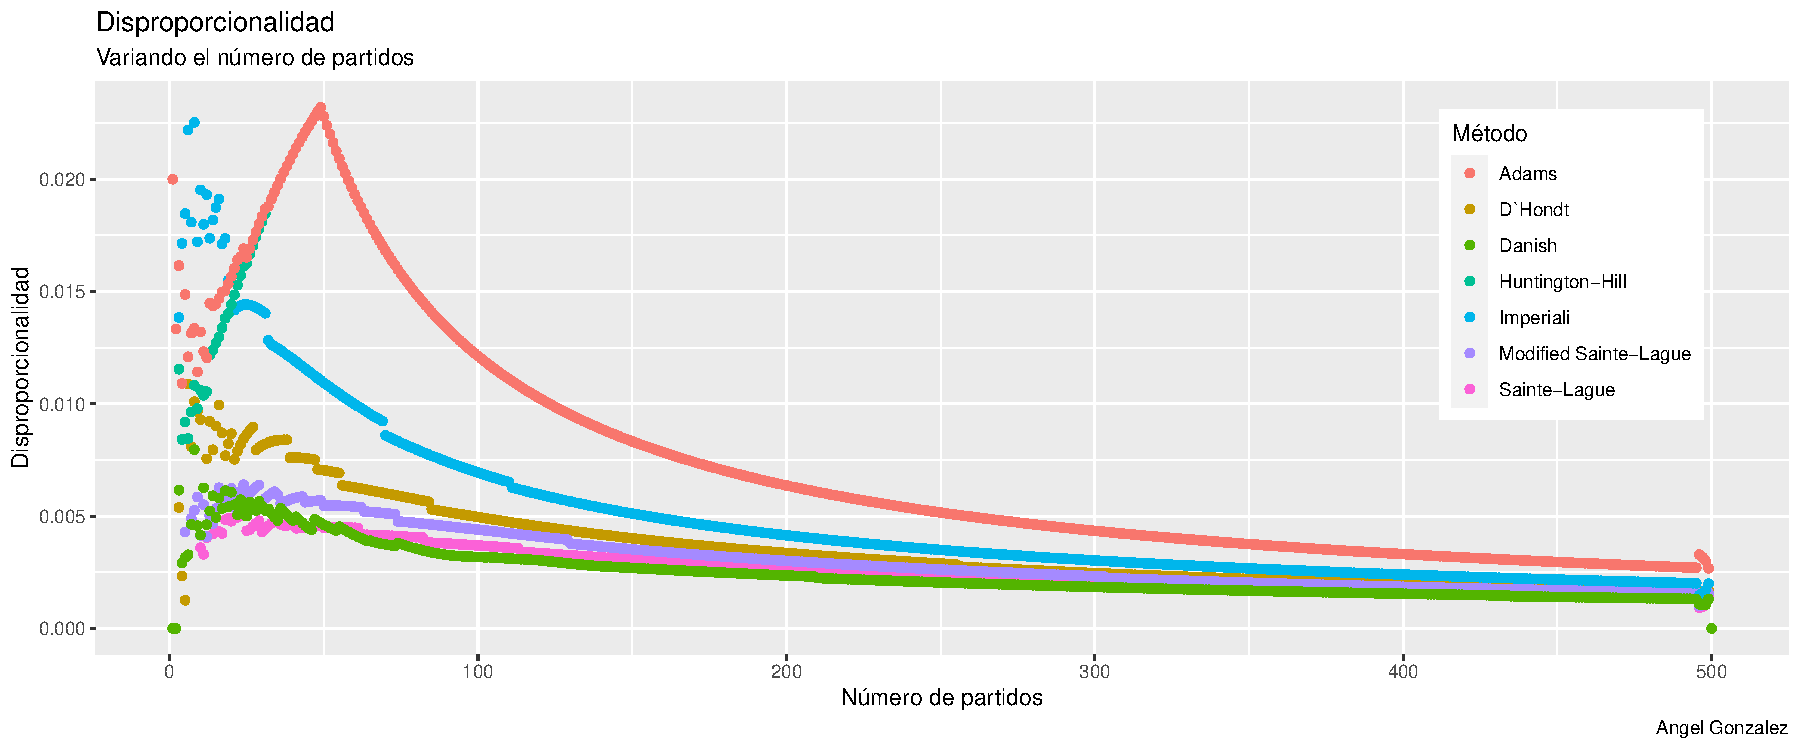
\includegraphics[width=0.95\linewidth]{figurasR/unnamed-chunk-44-1} \end{center}

En el presente gráfico comparamos la disproporcionalidad variando el
número de partidos en un mismo lugar con los métodos anteriormente
analizados individualmente.

Observamos que para un número de partidos bajo hasta los 50 partidos que
se presentan a unas elecciones la disproporcionalidad es muy variable, a
partir de los 50 partidos se estabiliza y podemos sacar algunas
conclusiones, en primer lugar el peor método claramente en este caso es
el método Adams, mientras que los demás métodos son muy similares en su
disproporcionalidad, donde la menor disproporcionalidad lo podemos
encontrar en el método Adams.

\begin{center}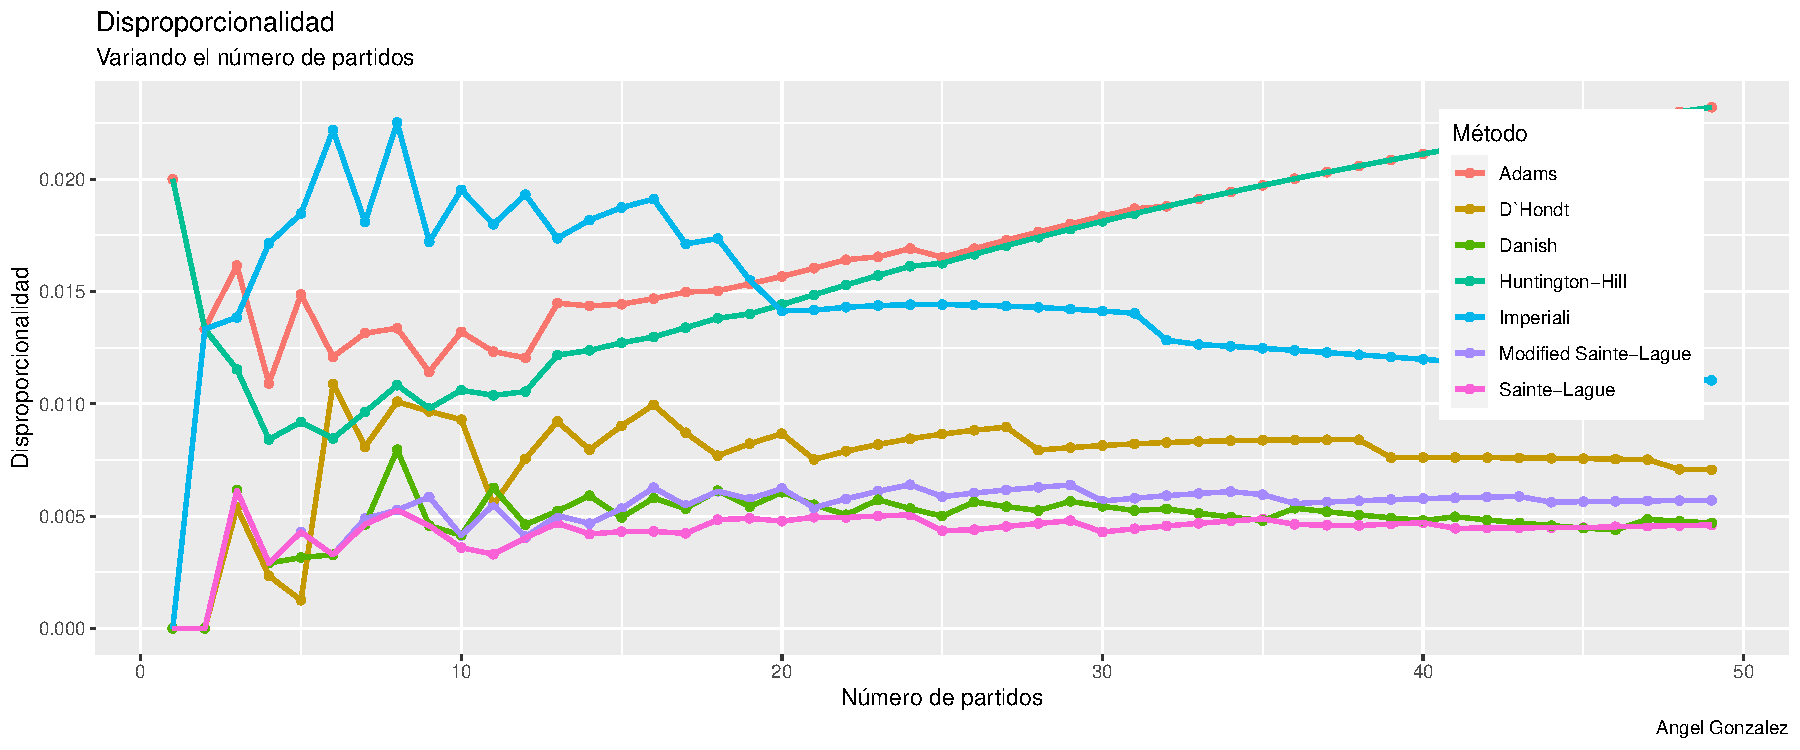
\includegraphics[width=0.95\linewidth]{figurasR/unnamed-chunk-45-1} \end{center}

En este gráfico nos centramos en la disproporcionalidad para un número
de partidos entre 2 y 50 partidos.

Observamos que hasta los 20 partidos que se presentan a las elecciones
la disproporcionalidad es muy variable entre ellos, a partir de los 20
partidos que se presentan en las elecciones podemos extraer algunas
conclusiones, se ven dos grupor direfenciados, un grupo en donde la
disproporcionalidad es estable e incluso decreciente y otro grupo en el
que la disproporcionalidad va aumentando, que son los métodos de Adams y
Huntington-Hill.

En España se utiliza el método D´Hondt, según los datos obtenidos
podemos concluir que el método d´Hondt no es el mejor método entre los
analizados, sería el cuarto mejor método entre siete métodos posibles,
es decir, sería deseable para obtener una mayor proporcionalidad que se
cambiase el método de reparto a otro mejor, en este caso observamos que
el mejor método es el Saint-Lague.

\hypertarget{variando-la-distribuciuxf3n-de-los-votos}{%
\subsection{Variando la distribución de los
votos}\label{variando-la-distribuciuxf3n-de-los-votos}}

\begin{center}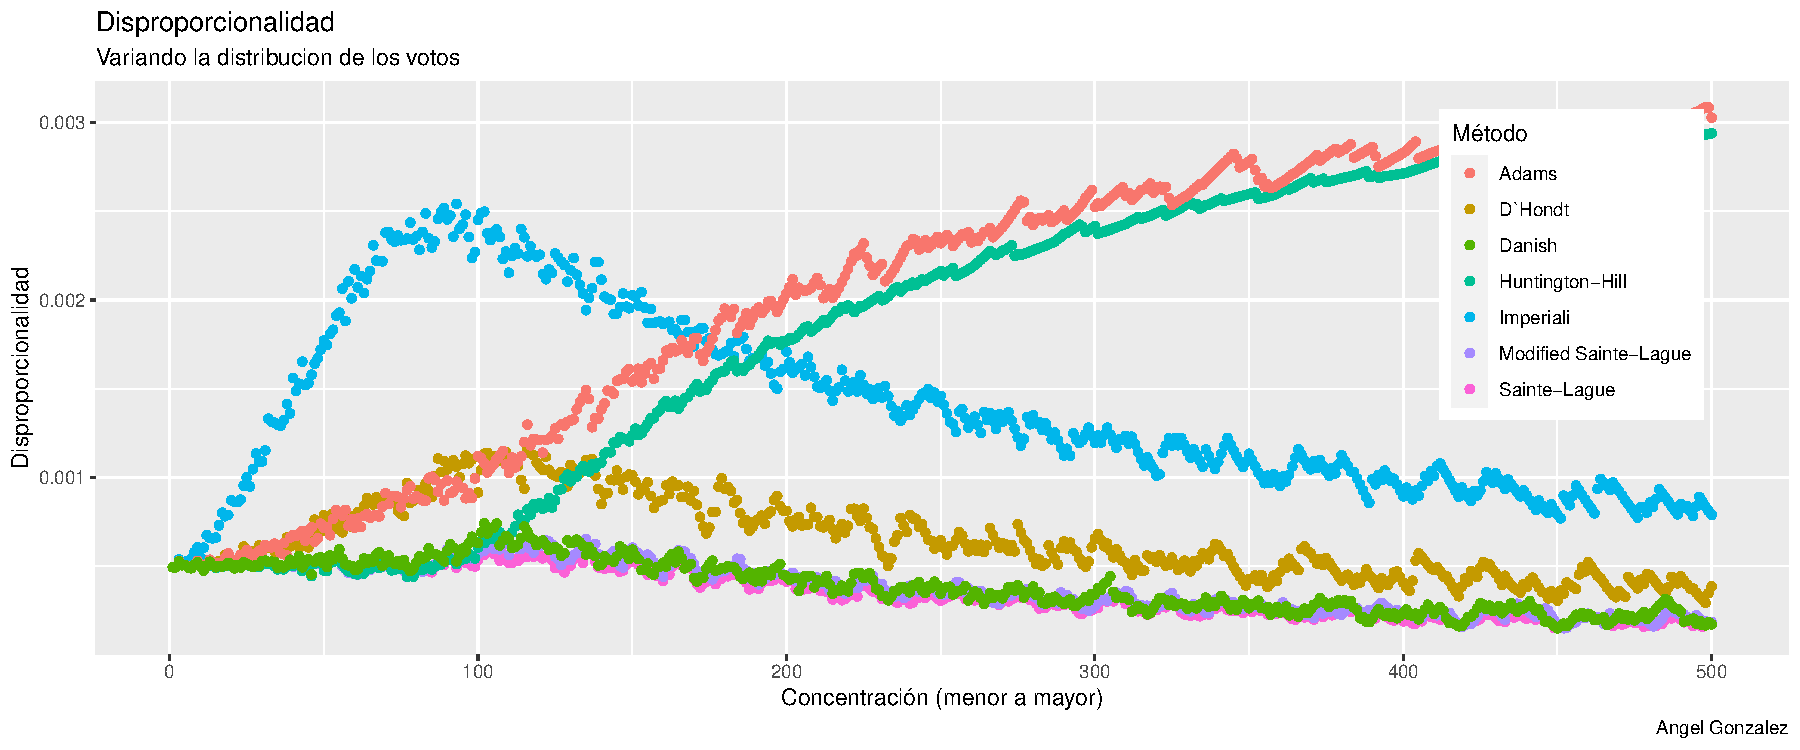
\includegraphics[width=0.95\linewidth]{figurasR/unnamed-chunk-46-1} \end{center}

En el presente gráfico comparamos la distribución de los votos en unas
elecciones ficticias, comenzamos con una concentración de votos baja, es
decir, la diferencia de votos entre partidos es baja, hasta acabar con
una concentración de votos alta, en donde la diferencia de votos entre
partidos es muy grande. Todo ello en un mismo lugar con los métodos
anteriormente analizados individualmente.

Observamos que hay dos grupos diferenciados, uno de ellos en los que la
disproporcionalidad es baja para una menor concentración de votos entre
los partidos y que a medida que la concentración aumenta también va
aumentando la disproporcionalidad, donde se encuentran los métodos de
Adams y Huntington-Hill. El otro grupo se caracteriza por en cuanto la
concentración del voto es muy baja la disproporcionalidad está en un
nivel bajo, cuanto más concentración de voto podemos comprobar como la
disproporcionalidad aumenta hasta que alcanza un punto en donde alcanza
el máximo de disproporcionalidad y a partir de ese punto la
disproporcionalidad va bajando alcanzando el mínimo de
disproporcionalidad.

\begin{center}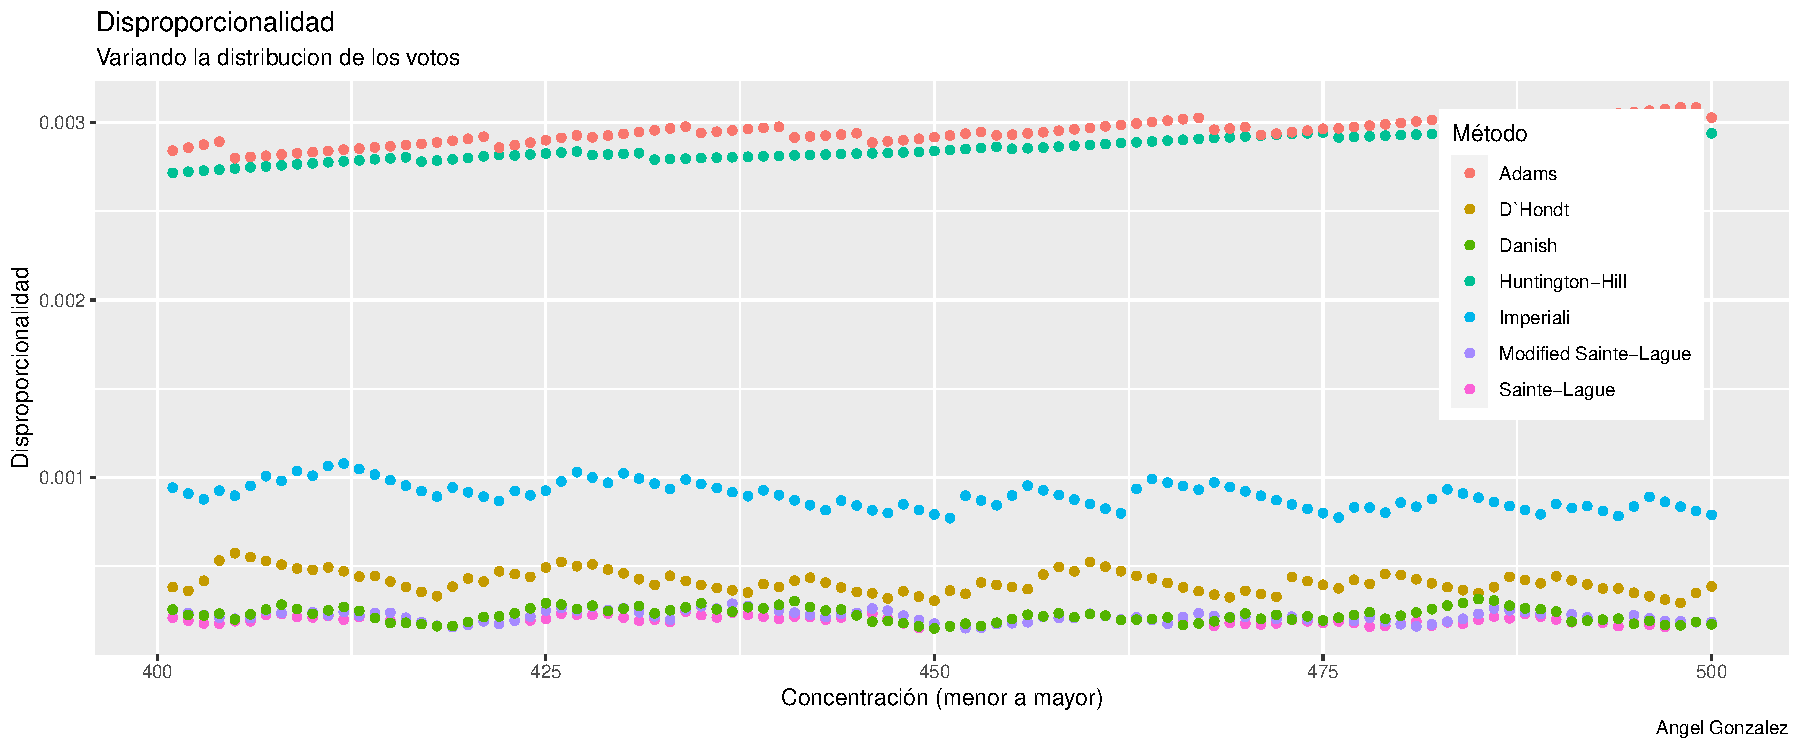
\includegraphics[width=0.95\linewidth]{figurasR/unnamed-chunk-47-1} \end{center}

En este gráfico nos centramos en los casos en que hay mayor
concentración de votos de unos pocos partidos, lo que suele suceder
actualmente. Vemos que hay dos grupos diferenciados, uno en el que hay
una alta disproporcionalidad, que serían los métodos Adams y
Huntington-Hill y otro en el que la disproporcionalidad es baja. En
España actualmente la concentración de voto en alta o medio-alta y se
utiliza el método de D´Hondt, por lo tanto observando el gráfico podemos
decir que el método utilizado en España no es el más optimo en el caso
de la concentración de voto actual en España, sería conveniente realizar
un cambio de método y cambiarlo preferentemente por el método
Sainte-Lague, que es el mejor entre los métodos del grupo con
disproporcionalidad baja.

\hypertarget{conclusiones}{%
\section{Conclusiones}\label{conclusiones}}

En general podemos concluir que una vez comparados todos los métodos
tanto modificando el número de escaños a repartir, en número de partidos
que se presentan a la elección y la concentración de los votos,
concluimos que el mejor método es el Saint-Lague, seguido por el
Modified Sainte-Lague y el Danish. En el caso del método utilizado
actualmente en España, el método D´hondt, podemos decir que es un método
que no siendo de los peores se queda en un medio que no es ni un método
malo ni bueno, es decir, que no es un método que se debiese usar, puesto
que no es el mejor en ninguno de las posibles modificaciones que se
presentan en este estudio, siendo entonces conveniente para España
cambiar el método de reparto de escaños y utilizar el método de
Sainte-Lague que es el que consistentemente ha presentado los mejores
resultados.

\FloatBarrier

\ifdefined\ifprincipal
\else
\setlength{\parindent}{1em}
\pagestyle{fancy}
\setcounter{tocdepth}{4}
\tableofcontents

\fi

\ifdefined\ifdoblecara
\fancyhead{}{}
\fancyhead[LE,RO]{\scriptsize\rightmark}
\fancyfoot[LO,RE]{\scriptsize\slshape \leftmark}
\fancyfoot[C]{}
\fancyfoot[LE,RO]{\footnotesize\thepage}
\else
\fancyhead{}{}
\fancyhead[RO]{\scriptsize\rightmark}
\fancyfoot[LO]{\scriptsize\slshape \leftmark}
\fancyfoot[C]{}
\fancyfoot[RO]{\footnotesize\thepage}
\fi
\renewcommand{\headrulewidth}{0.4pt}
\renewcommand{\footrulewidth}{0.4pt}

\hypertarget{analisis-de-los-datos}{%
\chapter{Analisis de los datos}\label{analisis-de-los-datos}}

\hypertarget{auxf1o-1977}{%
\section{Año 1977}\label{auxf1o-1977}}

\hypertarget{comparativa-entre-muxe9todos}{%
\subsection{Comparativa entre
métodos}\label{comparativa-entre-muxe9todos}}

\hypertarget{votos-obtenidos}{%
\subsubsection{Votos obtenidos}\label{votos-obtenidos}}

\begin{center}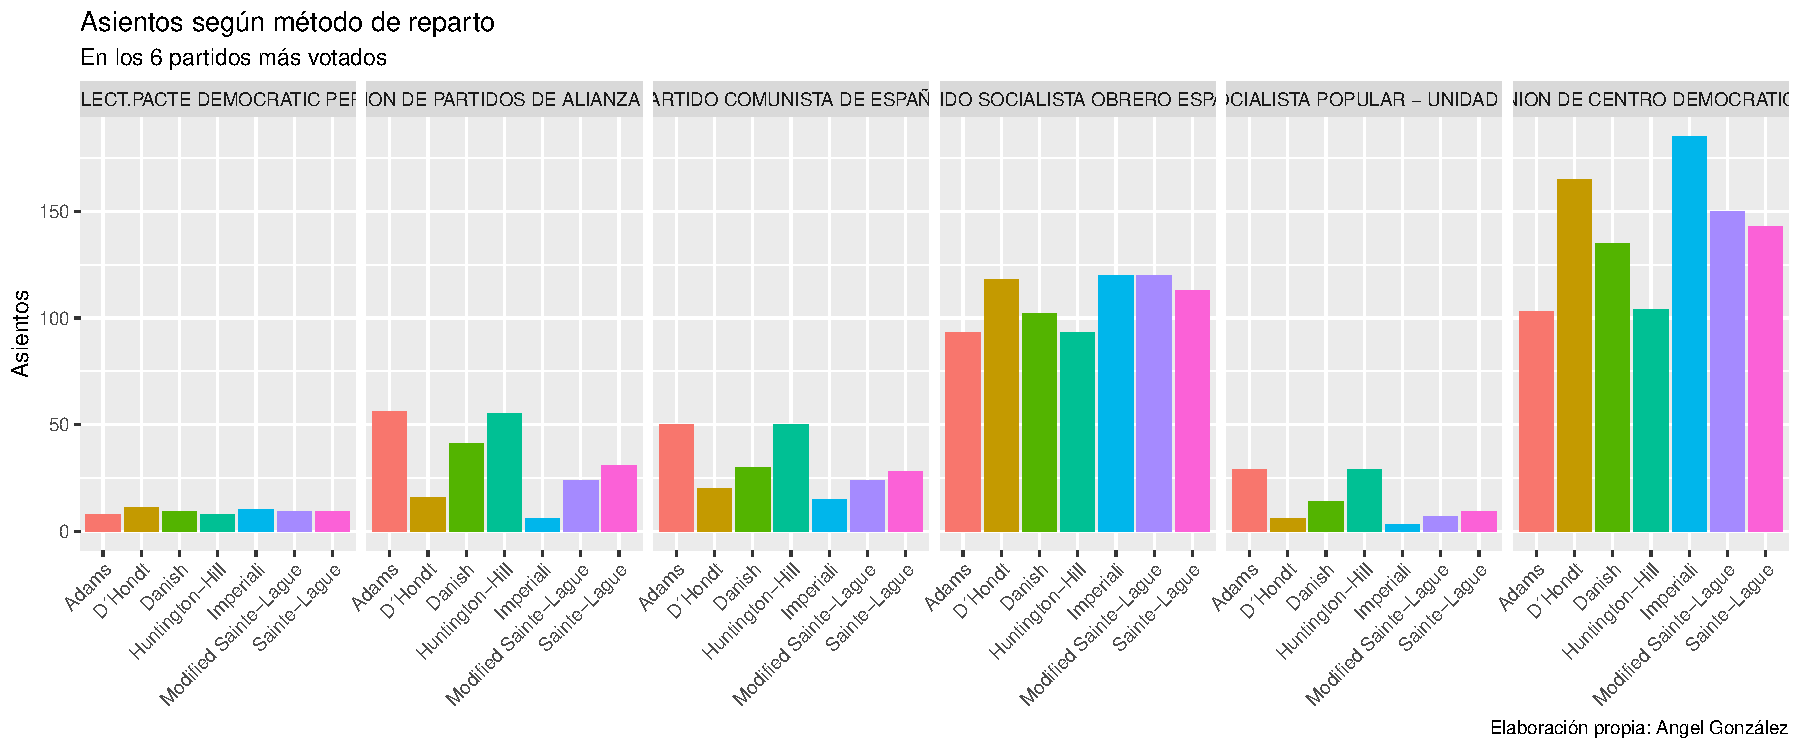
\includegraphics[width=0.95\linewidth]{figurasR/unnamed-chunk-59-1} \end{center}

\begin{center}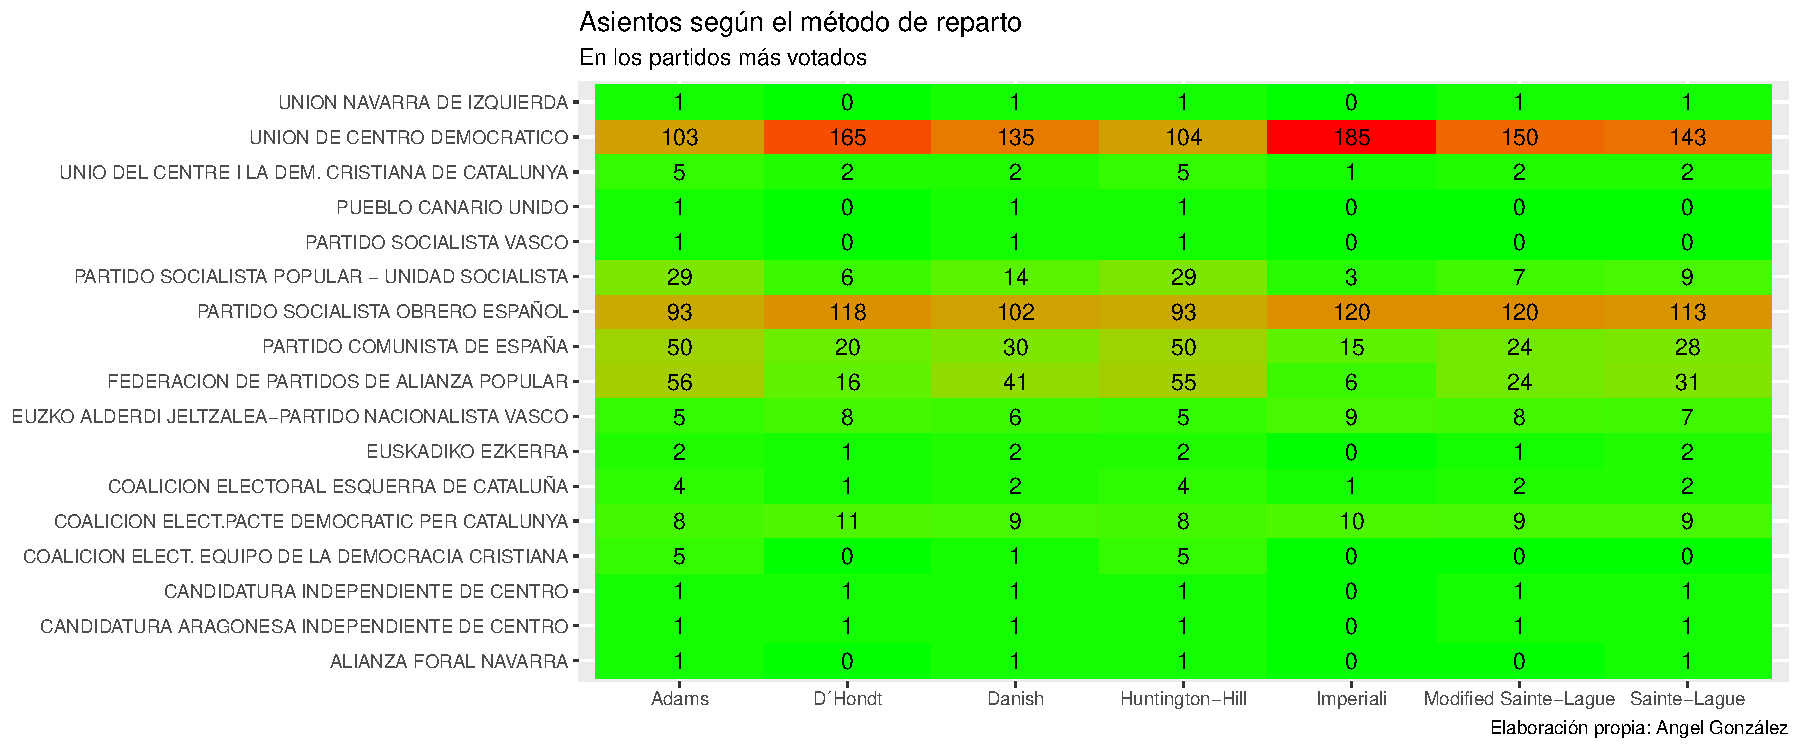
\includegraphics[width=0.95\linewidth]{figurasR/unnamed-chunk-59-2} \end{center}

En estas primeras elecciones de 1977 podemos observar que la fuerza más
votada en las elecciones es el partido \emph{Unión de Centro
democrático} seguido del \emph{PSOE}. Observamos que según el método
vigente en España, el método D´Hondt, el partido \emph{UCD}, que ganaría
las elecciones, tendría una gran diferencia de votos respecto a los
demás partidos, por lo que facilitaría la gobernabilidad.

Comparando entre métodos de reparto observamos que el que más escaños da
a los partidos grandes es el método imperiali, que beneficia mucho a los
partidos más votados y penaliza mucho en escaños a los partidos tanto
medianos como poco votados. El método actual en España también tiene un
comportamiento similar al imperiali aunque no tan acusado. En la otra
parte de la balanza encontramos al método Adams, el cual da muy pocos
escaños al partidos más votado y a los partidos medianos les beneficia.

En estas elecciones no se obtiene la mayoría absoluta en ningún método
excepto en el método imperiali, en los demás métodos el partido ganador
debería de aliarse con uno o dos partidos para obtener la mayoría
absoluta, los grandes perdedores en términos de escaños obtenidos son el
partido comunista y Alianza Popular, que podrían obtener hasta 10
escaños más de haber optado por otro método de reparto de votos.

\hypertarget{disproporcionalidad}{%
\subsubsection{Disproporcionalidad}\label{disproporcionalidad}}

\begin{center}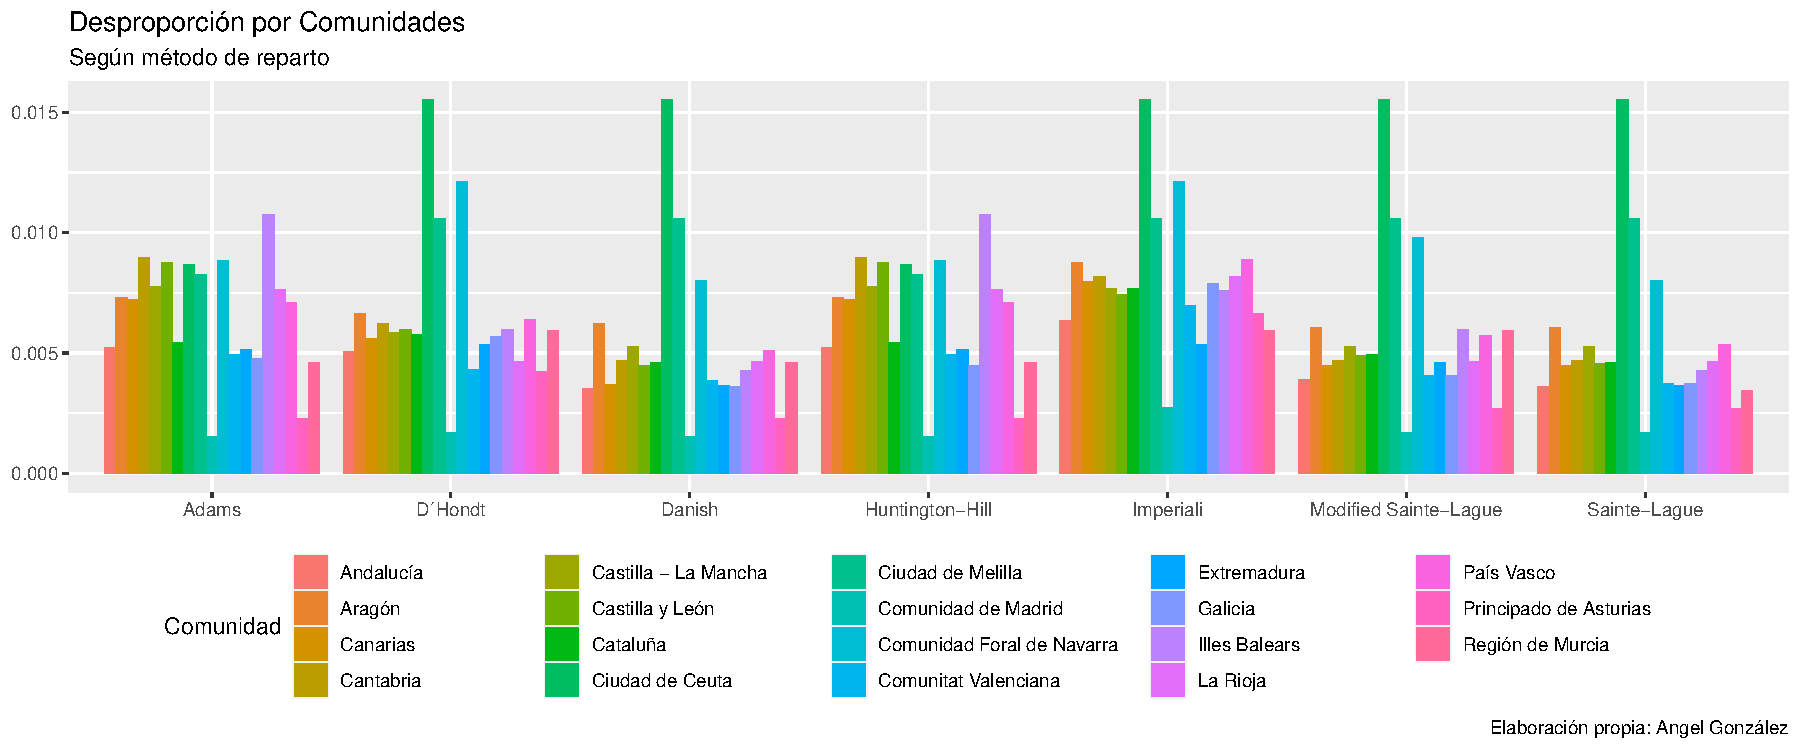
\includegraphics[width=0.95\linewidth]{figurasR/unnamed-chunk-60-1} \end{center}

\begin{center}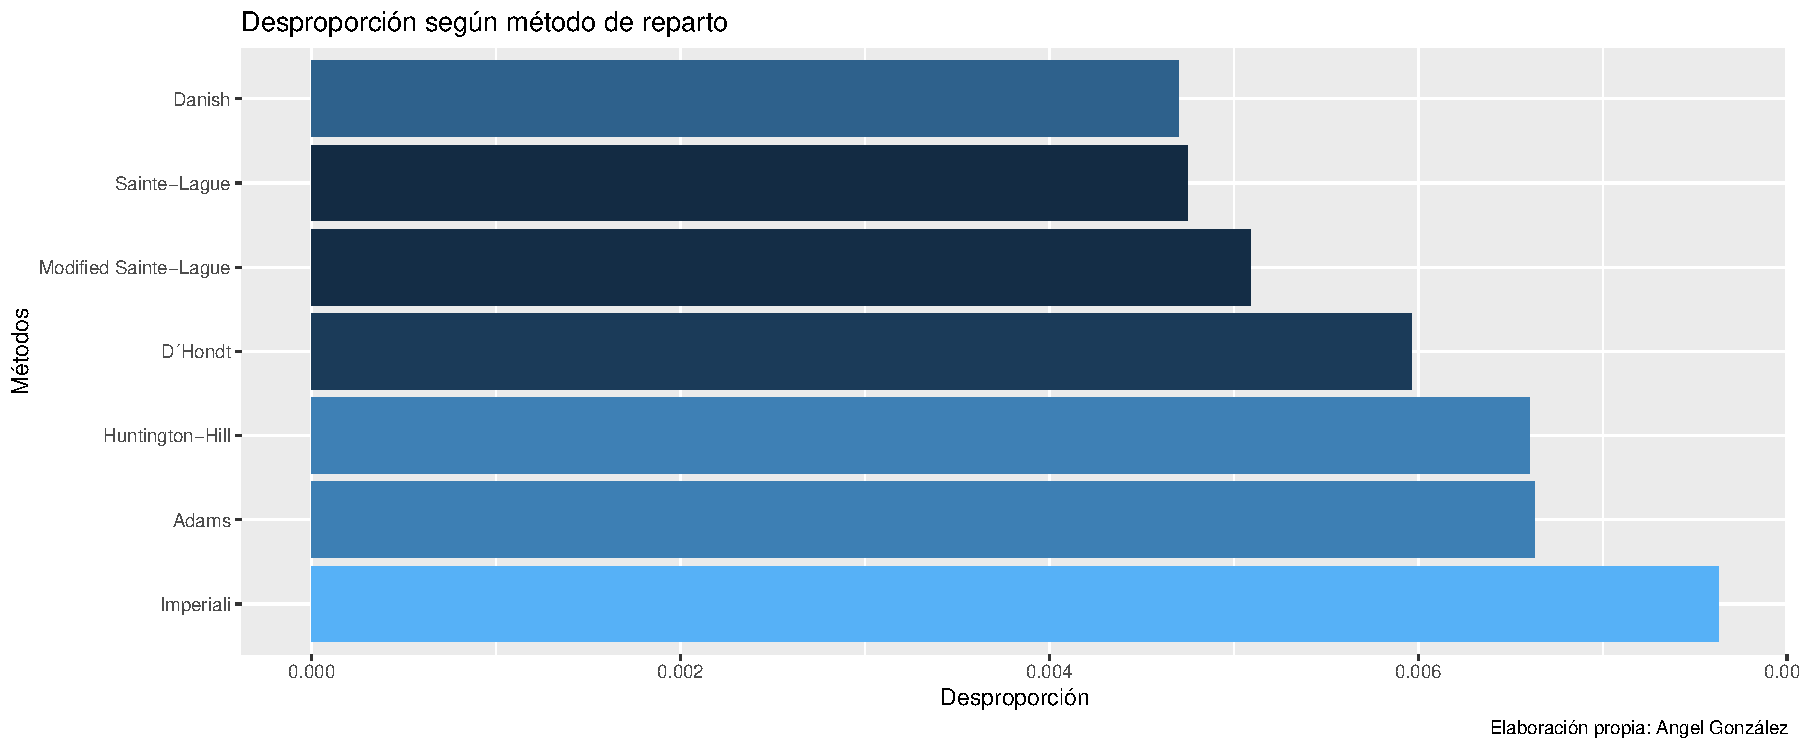
\includegraphics[width=0.95\linewidth]{figurasR/unnamed-chunk-60-2} \end{center}

En el presente gráfico, en el que se mide la desproporcionalidad por
comunidades, observamos que en general entre todos los métodos las
comunidades más desproporcionadas son las ciudades de Ceuta y Melilla,
resultado lógico en tanto que al repartirse un único escaño es el
partido más votado únicamente el que obtiene el escaño. Es común entre
todos los métodos que la comunidad de Madrid sea la comunidad más
proporcionada, esto es debido a que es la comunidad en la que se
reparten más asientos y también la más poblada, por lo que cuando se
reparten los asientos por provincias, al utilizar el método D´Hondt,
como hemos visto beneficia a los lugares con más población. En general
los métodos que presentan una menor diferencia de disproporcionalidad
entre las distintas comunidades autónomas son el método Danish y el
Saint-Lague, en cambio las que presentan una mayor diferencia entre
comunidades son el método Adams y el Huntington-Hill.

Si nos centramos en el gráfico de la disproporcionalidad media según el
método de reparto podemos observar que la menor disproporcionalidad se
encuentra en los métodos Danish y Sainte-Lague, mientras que las mayores
disproporcionalidades se encuentran en el método Imperiali y Adams.
Especial caso hacemos al método D´Hondt al ser el método utilizado
actualmente en España, observamos que ni es el mejor método ni tampoco
es de los peores, debido a ello sería conveniente cambiar el método de
reparto a otro mejor, que podría ser o bien el Sainte-Lague o el Danish.

\hypertarget{auxf1o-1979}{%
\section{Año 1979}\label{auxf1o-1979}}

\hypertarget{comparativa-entre-muxe9todos-1}{%
\subsection{Comparativa entre
métodos}\label{comparativa-entre-muxe9todos-1}}

\hypertarget{votos-obtenidos-1}{%
\subsubsection{Votos obtenidos}\label{votos-obtenidos-1}}

\begin{center}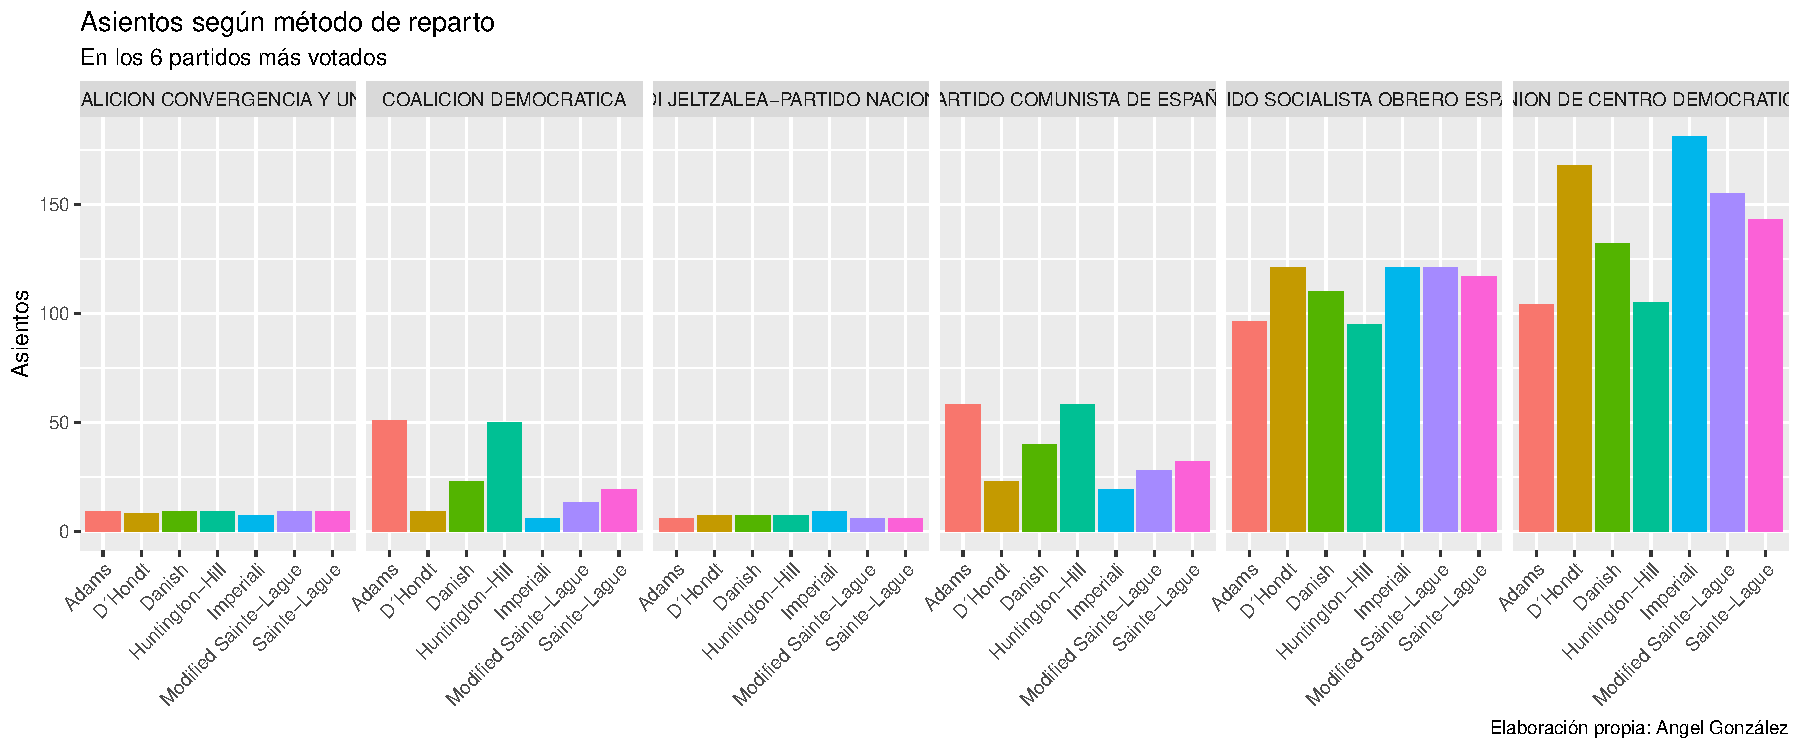
\includegraphics[width=0.95\linewidth]{figurasR/unnamed-chunk-68-1} \end{center}

\begin{center}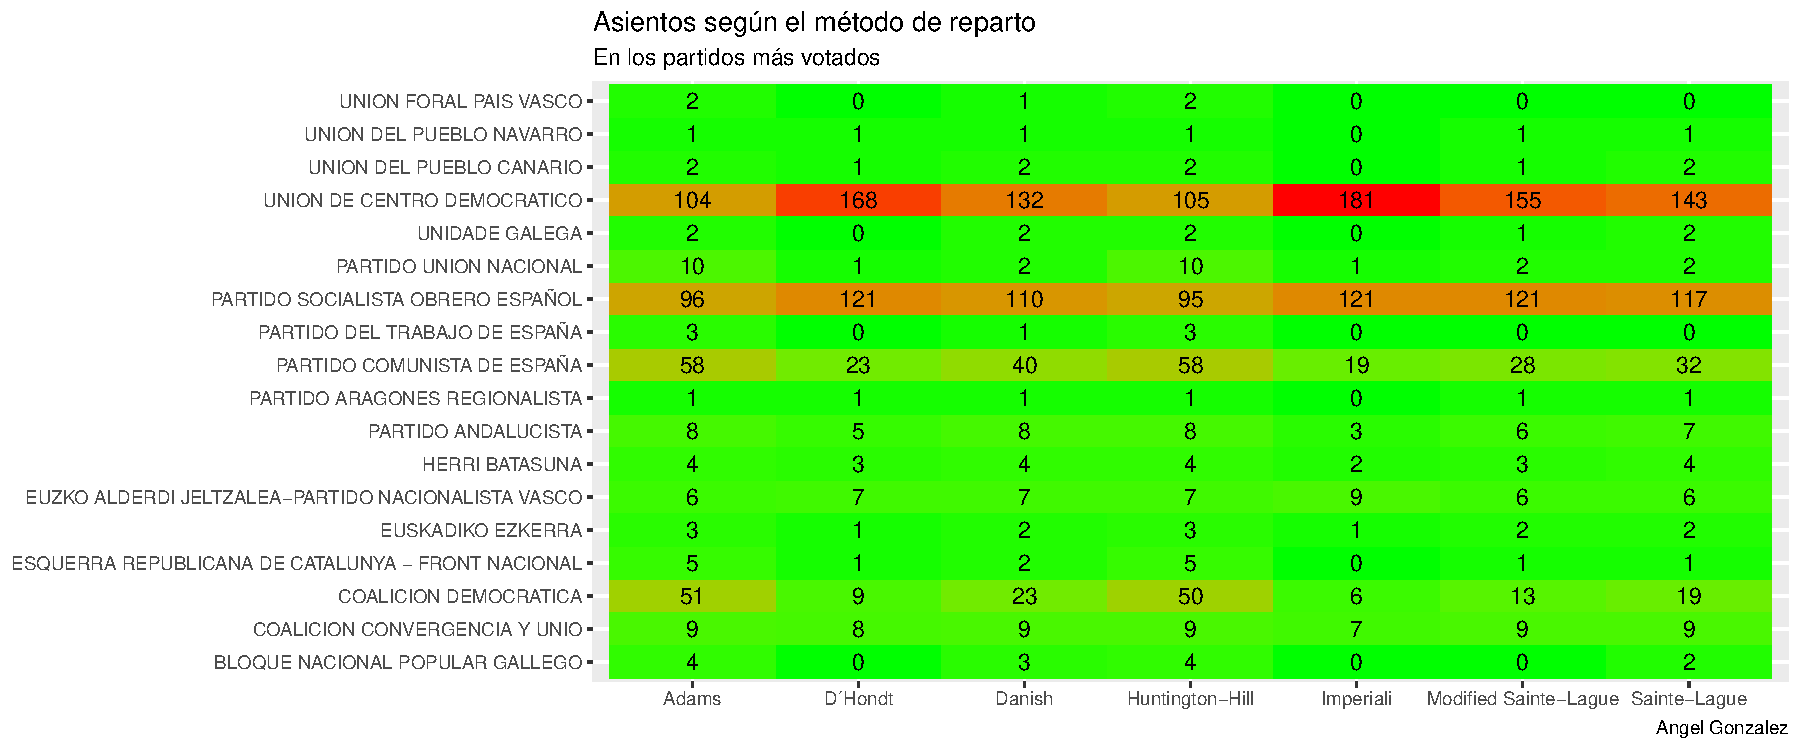
\includegraphics[width=0.95\linewidth]{figurasR/unnamed-chunk-68-2} \end{center}

En estas elecciones de 1979 el partido más votado fué \emph{UCD} seguido
del \emph{PSOE}, según los distintos métodos de reparto únicamente en el
método Imperiali UCD conseguiría la mayoría absoluta, en todos los demás
métodos de reparto no se alcanza la mayoría absoluta, los partidos más
castigados por utilizar el método D´Hondt son el partido comunista y
coalición Democrática, que podrían hasta doblar el número de asientos
obtenidos dependiendo del método de reparto que se haya realizado. En
estas elecciones podemos decir que hay dos grandes partidos y dos
medianos, UCD y el PSOE son los más grandes y el partido comunista y
coalición democrática son los partidos medianos, después ya se
encuentran todos los demás.

\hypertarget{disproporcionalidad-1}{%
\subsubsection{Disproporcionalidad}\label{disproporcionalidad-1}}

\begin{center}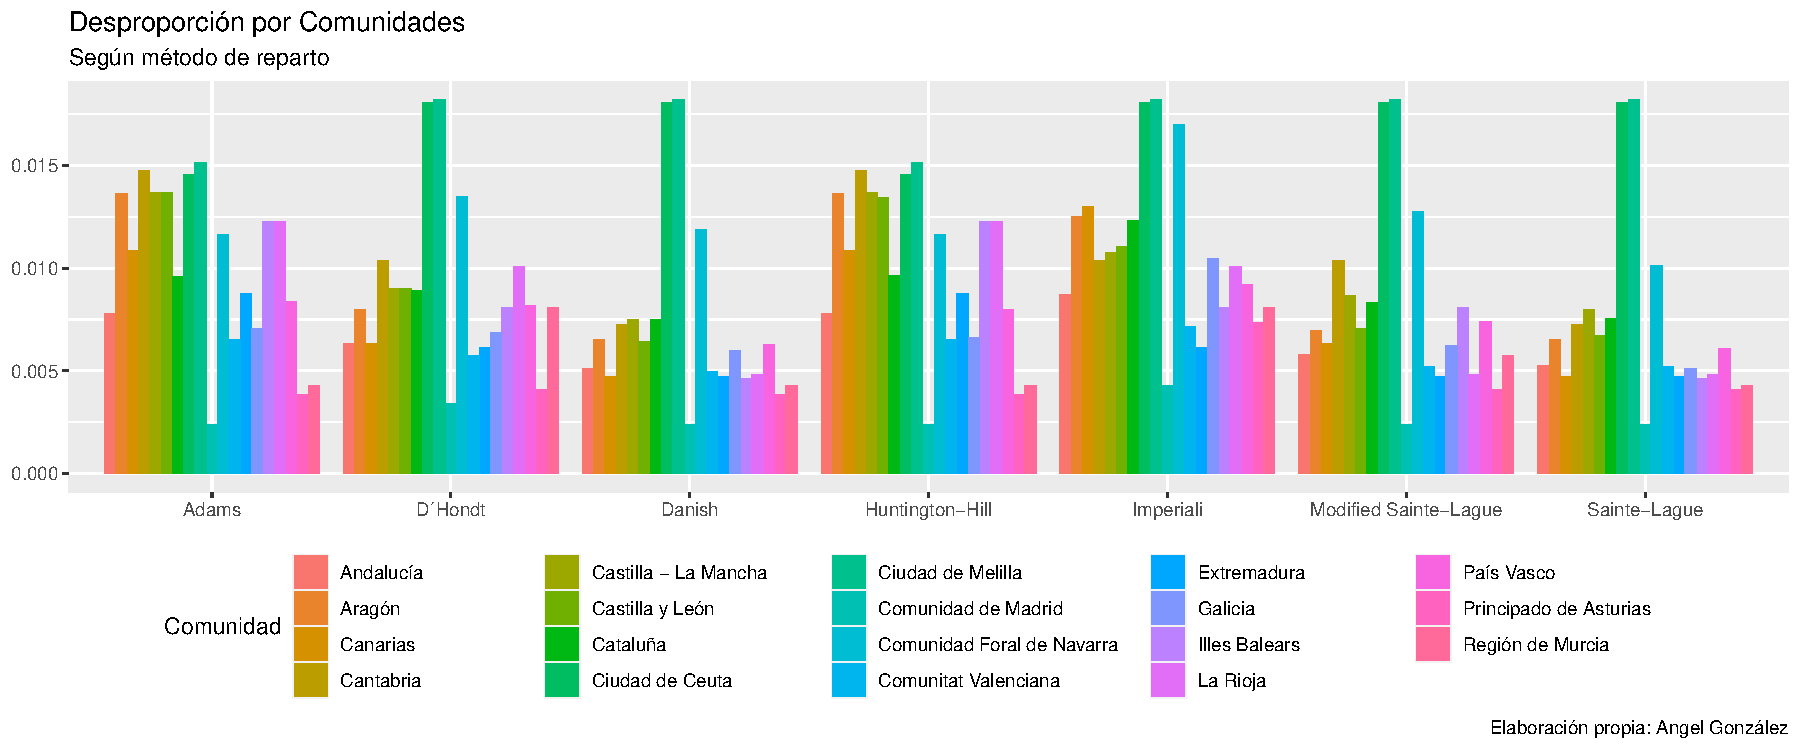
\includegraphics[width=0.95\linewidth]{figurasR/unnamed-chunk-69-1} \end{center}

\begin{center}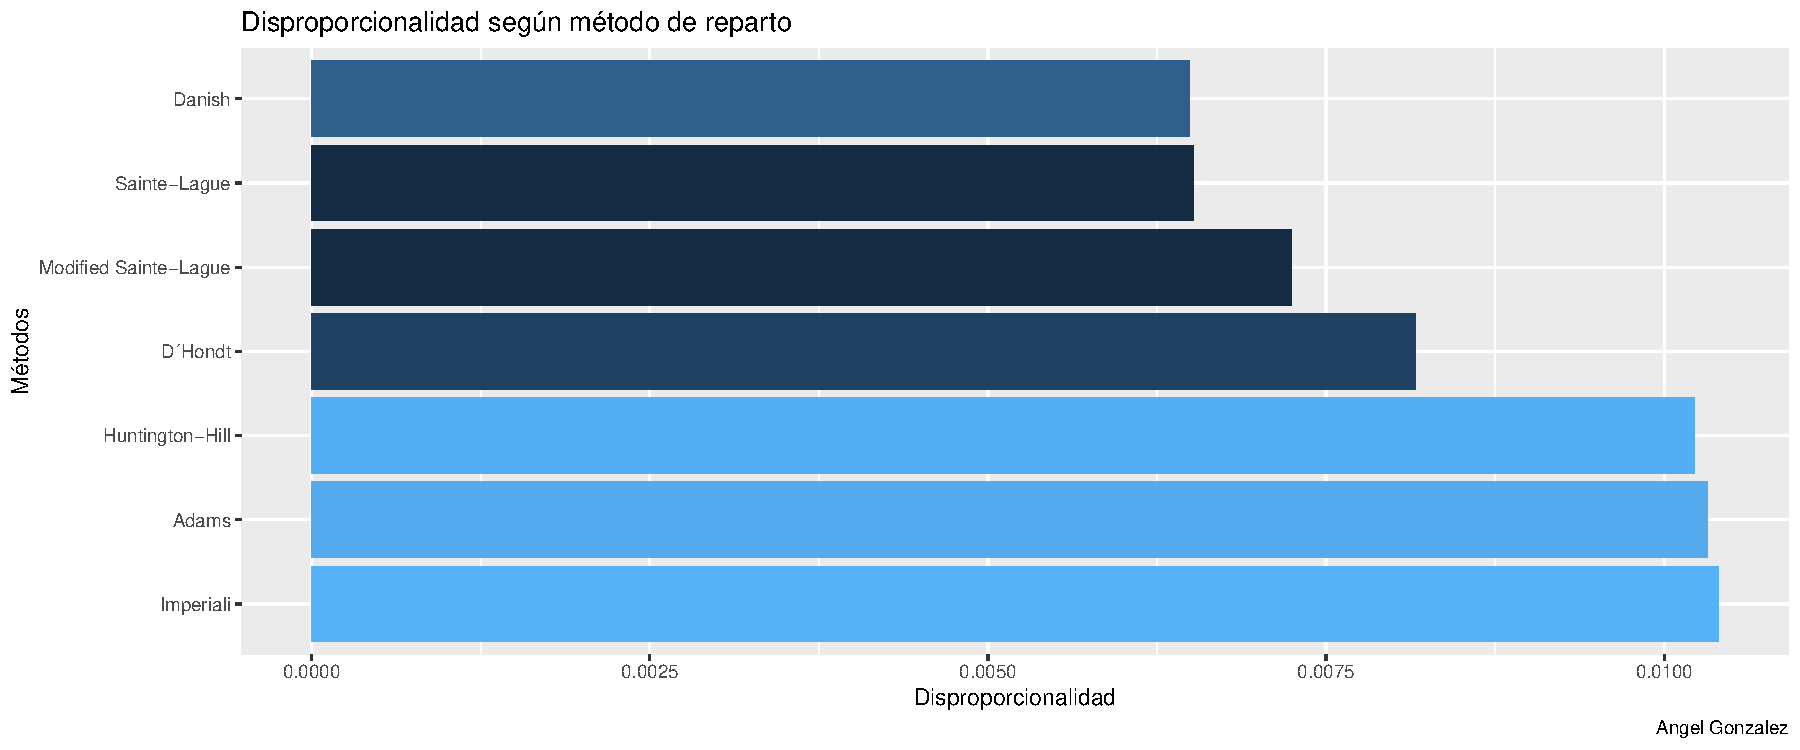
\includegraphics[width=0.95\linewidth]{figurasR/unnamed-chunk-69-2} \end{center}

En el presente gráfico vemos como respecto a las anteriores elecciones
hay una mayor diferencia de disproporcionalidad entre comunidades,
siguen teniendo las ciudades de Ceuta y Melilla la mayor
disproporcionalidad y la comunidad de Madrid la menor
disproporcionalidad.

Según la disproporcionalidad media los peores métodos de reparto se
pueden agrupar en tres, el método Imperiali, el Huntington-Hill, y el
Adams, y los mejores métodos de reparto en dos métodos, el Danish y el
Sainte-Lague. En el caso del método D´Hondt se encuentra en un término
medio, por lo que sería conveniente cambiar el método de reparto a uno
más proporcional, que puede ser el Danish o el Sainte-Lague.

\hypertarget{auxf1o-1982}{%
\section{Año 1982}\label{auxf1o-1982}}

\hypertarget{comparativa-entre-muxe9todos-2}{%
\subsection{Comparativa entre
métodos}\label{comparativa-entre-muxe9todos-2}}

\hypertarget{votos-obtenidos-2}{%
\subsubsection{Votos obtenidos}\label{votos-obtenidos-2}}

\begin{center}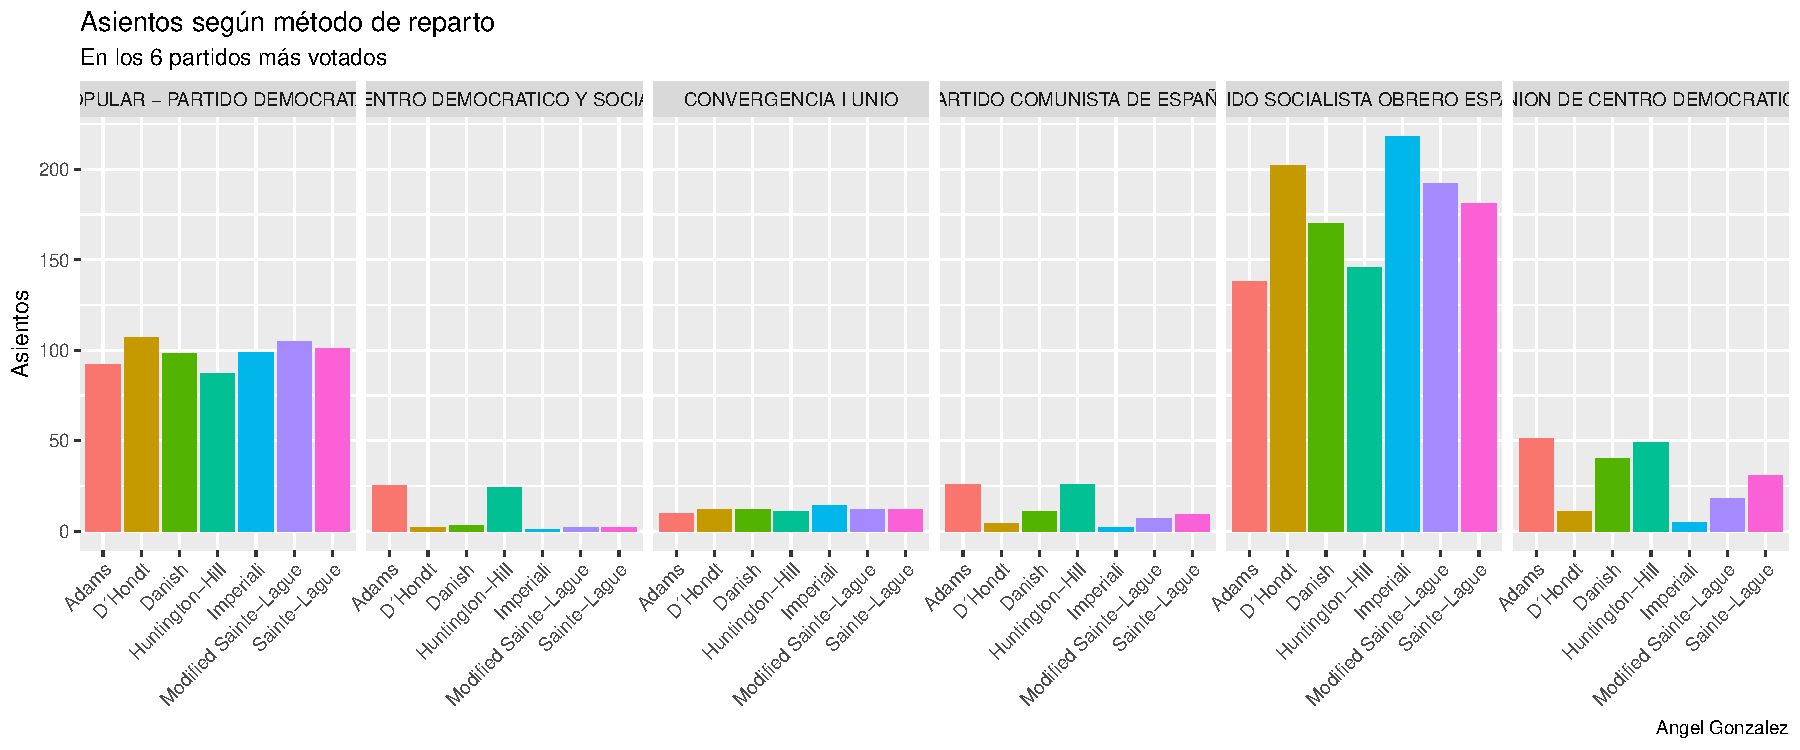
\includegraphics[width=0.95\linewidth]{figurasR/unnamed-chunk-77-1} \end{center}

\begin{center}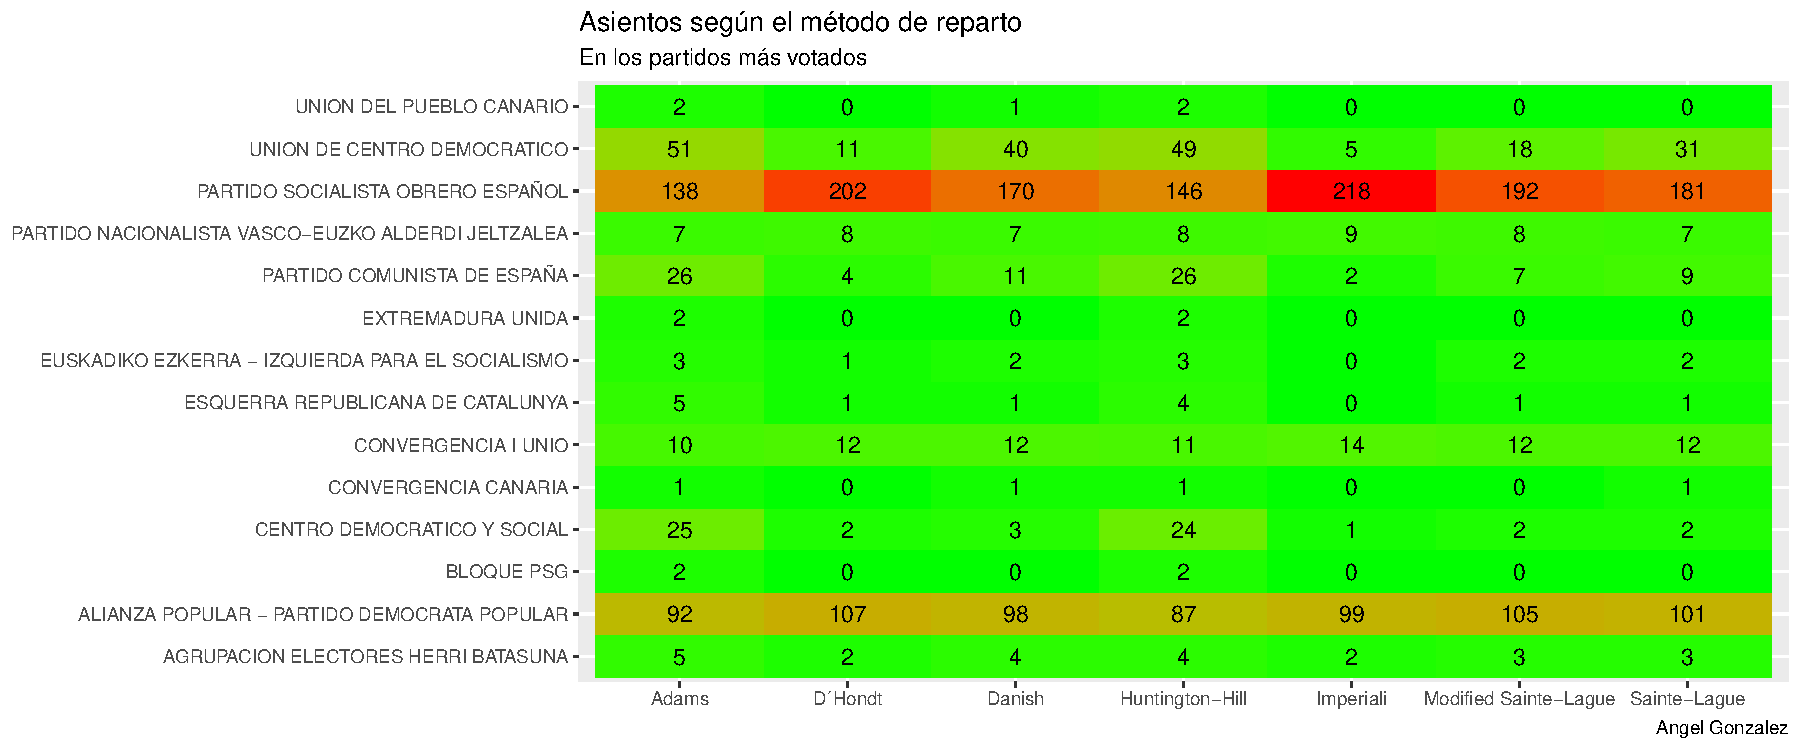
\includegraphics[width=0.95\linewidth]{figurasR/unnamed-chunk-77-2} \end{center}

En estas elecciones de 1982 el partido más votado es el \emph{PSOE} el
cual según la mayoría de los métodos de reparto, incluido el método
D´Hondt, alcanza la mayoría absoluta. Son unas elecciones en los que el
voto se concentra únicamente en dos partidos, que son el PSOE y Alianza
Popular, pero con una gran diferencia de asientos entre ellos, donde el
PSOE casi dobla en escaños a Alianza Popular. El partido menos
beneficiado en este año es UCD, que según el método D´Hondt obtendría 11
escaños mientras que si se optase por otro método más proporcional como
puede ser el método Danish o bien el Sainte-Lague podría multiplicar por
3 o 4 sus escaños.

\hypertarget{disproporcionalidad-2}{%
\subsubsection{Disproporcionalidad}\label{disproporcionalidad-2}}

\begin{center}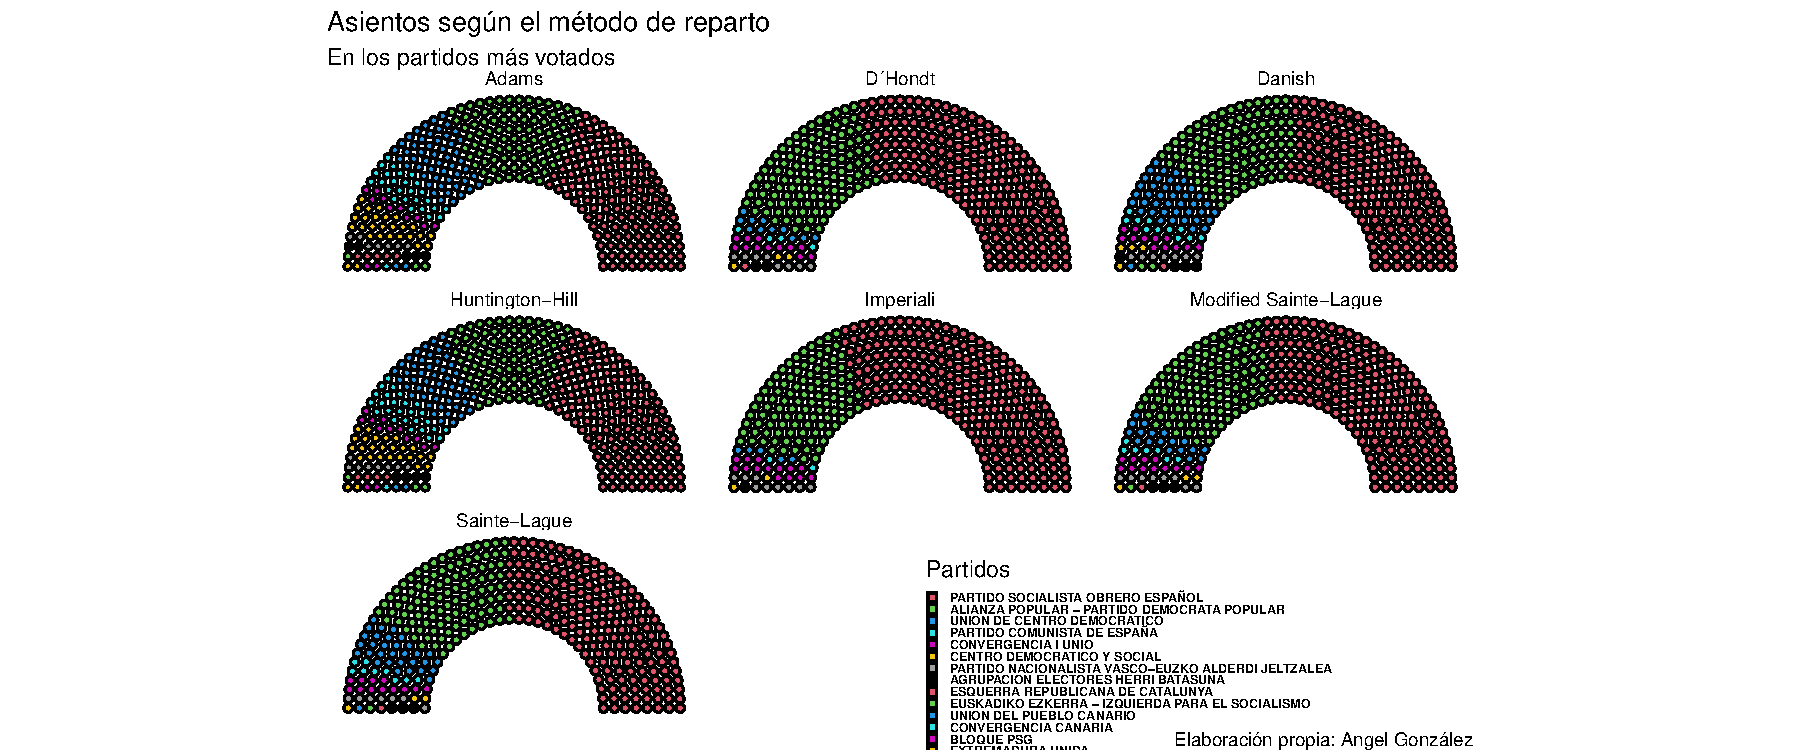
\includegraphics[width=0.95\linewidth]{figurasR/unnamed-chunk-78-1} \end{center}

\begin{center}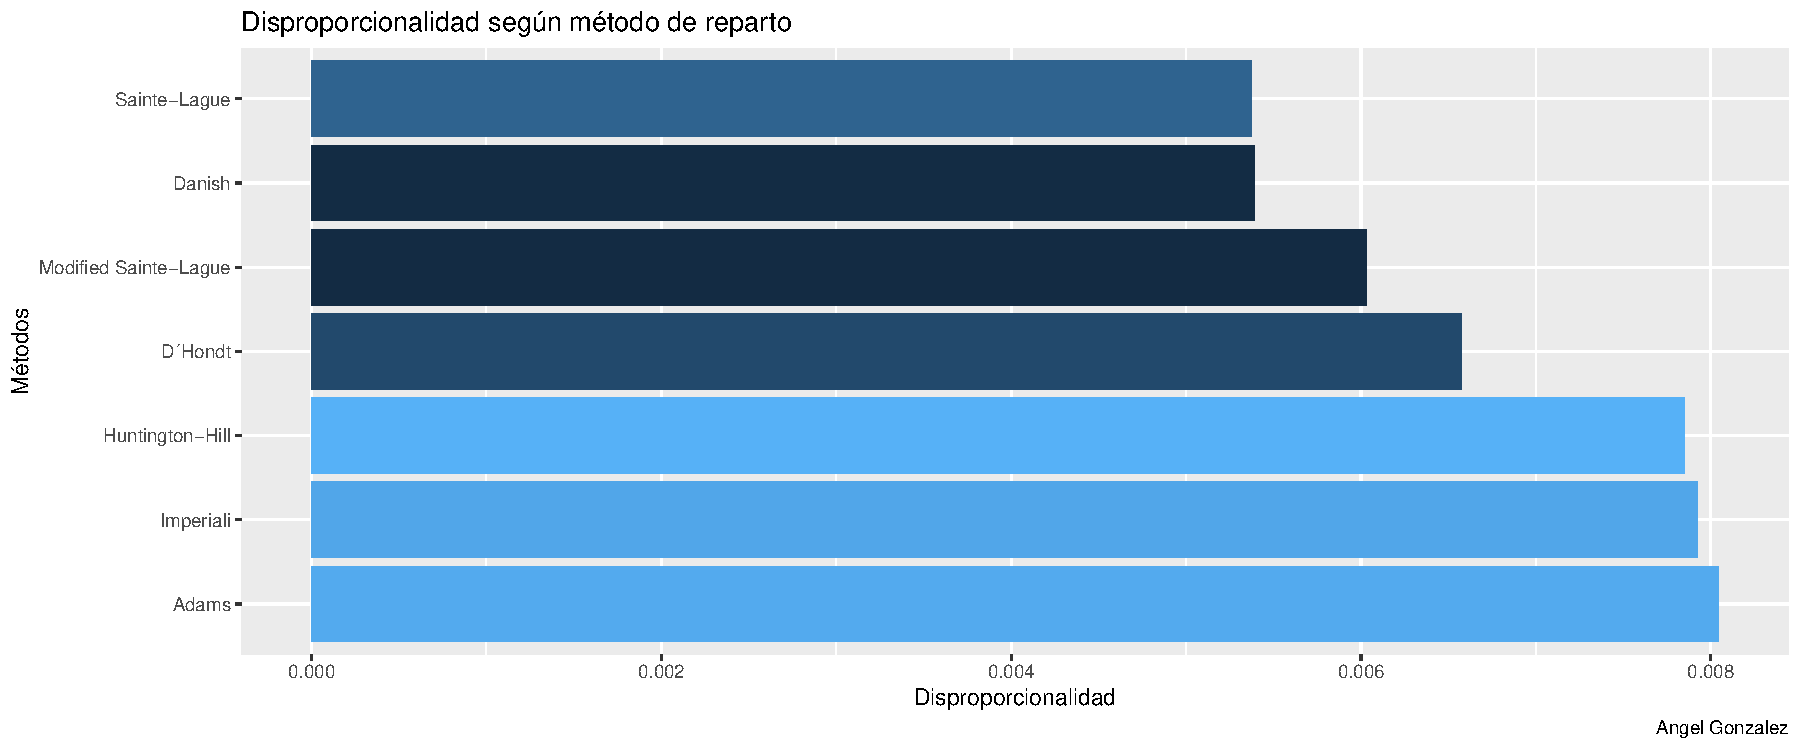
\includegraphics[width=0.95\linewidth]{figurasR/unnamed-chunk-78-2} \end{center}

Según la gráfica de disproporcionalidad por comunidades es un año en el
que generalmente no hay mucha diferencia de disproporcionalidad entre
ellas, este año las comunidades más desproporcionadas son la comunidad
Foral de Navarra y Cantabria mientras que las comunidades más
proporcionadas son la comunidad de Madrid y la región de Murcia.

Según la disproporción media, se reconocen tres grupos distintos, un
grupo muy disproporcionado, con el método Imperiali como el más
disproporcionado, otro grupo medio en donde se encontraría el método
D´Hondt y un último grupo el cual sería el más proporcionado en el que
se encontraría el método Danish y el Saint-Lague.

\hypertarget{auxf1o-1986}{%
\section{Año 1986}\label{auxf1o-1986}}

\hypertarget{comparativa-entre-muxe9todos-3}{%
\subsection{Comparativa entre
métodos}\label{comparativa-entre-muxe9todos-3}}

\hypertarget{votos-obtenidos-3}{%
\subsubsection{Votos obtenidos}\label{votos-obtenidos-3}}

\begin{center}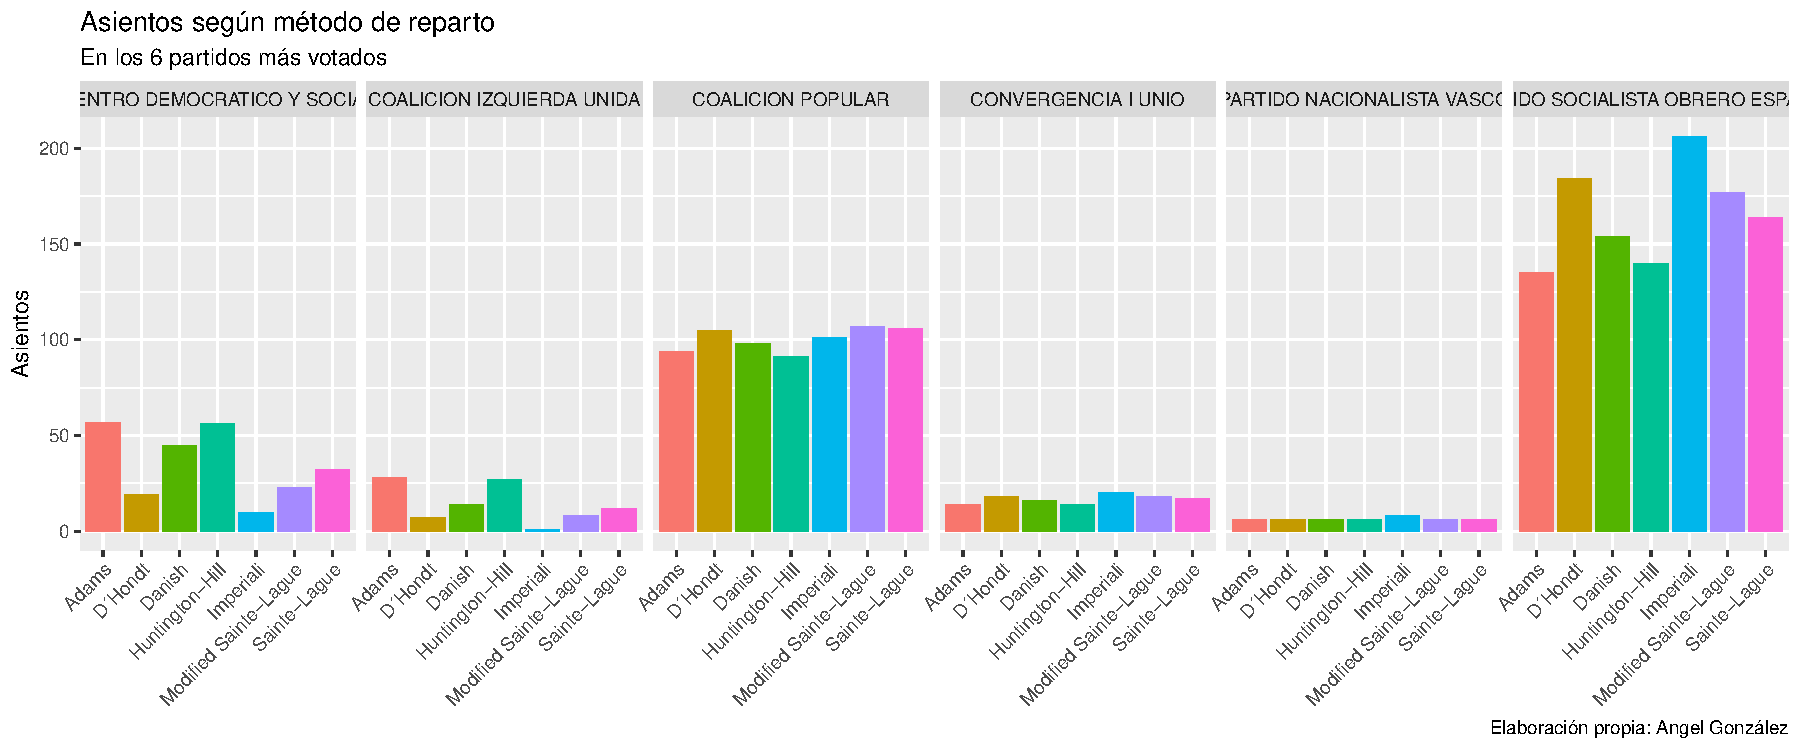
\includegraphics[width=0.95\linewidth]{figurasR/unnamed-chunk-86-1} \end{center}

\begin{center}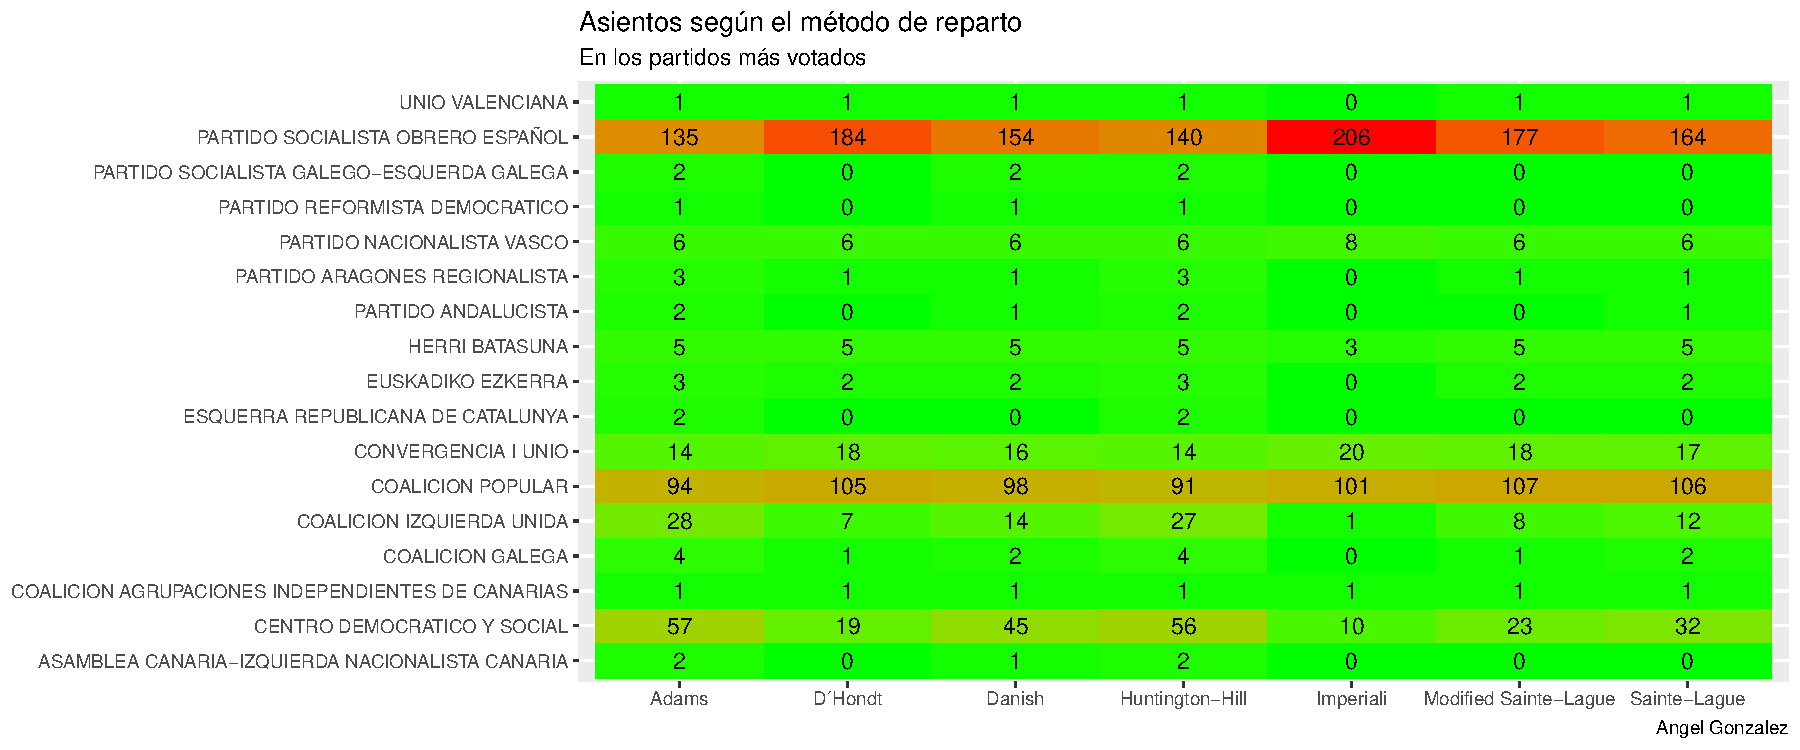
\includegraphics[width=0.95\linewidth]{figurasR/unnamed-chunk-86-2} \end{center}

En estas elecciones de 1986 el partido más votado fué el \emph{PSOE},
tal y como sucedió en las anteriores elecciones, son también unas
elecciones en donde hay únicamente dos partidos mayoritarios,
\emph{PSOE} y \emph{Coalición Popular}, ocurre en estas elecciones el
mismo escenario que en las anteriores elecciones, en donde el primer
partido casi dobla en escaños al segundo partido, aunque en este caso ya
se puede apreciar que la diferencia se va reduciendo entre los dos
grandes partidos, en general el PSOE alcanza la mayoría absoluta pero en
este año si utilizásemos los métodos más proporcionados es interesante
observar como perdería la mayoría absoluta tanto utilizando el método
Danish como el Sainte-Lague. Este año también reconocemos un partido que
podría decirse de nivel de votos medio que queda muy dañado por el
método de reparto D´Hondt, es el partido \emph{Centro Democrático y
Social}, el cual de utilizar los métodos más proporcionados podría hasta
duplicar sus escaños en el caso de optar por el método Danish.

\hypertarget{disproporcionalidad-3}{%
\subsubsection{Disproporcionalidad}\label{disproporcionalidad-3}}

\begin{center}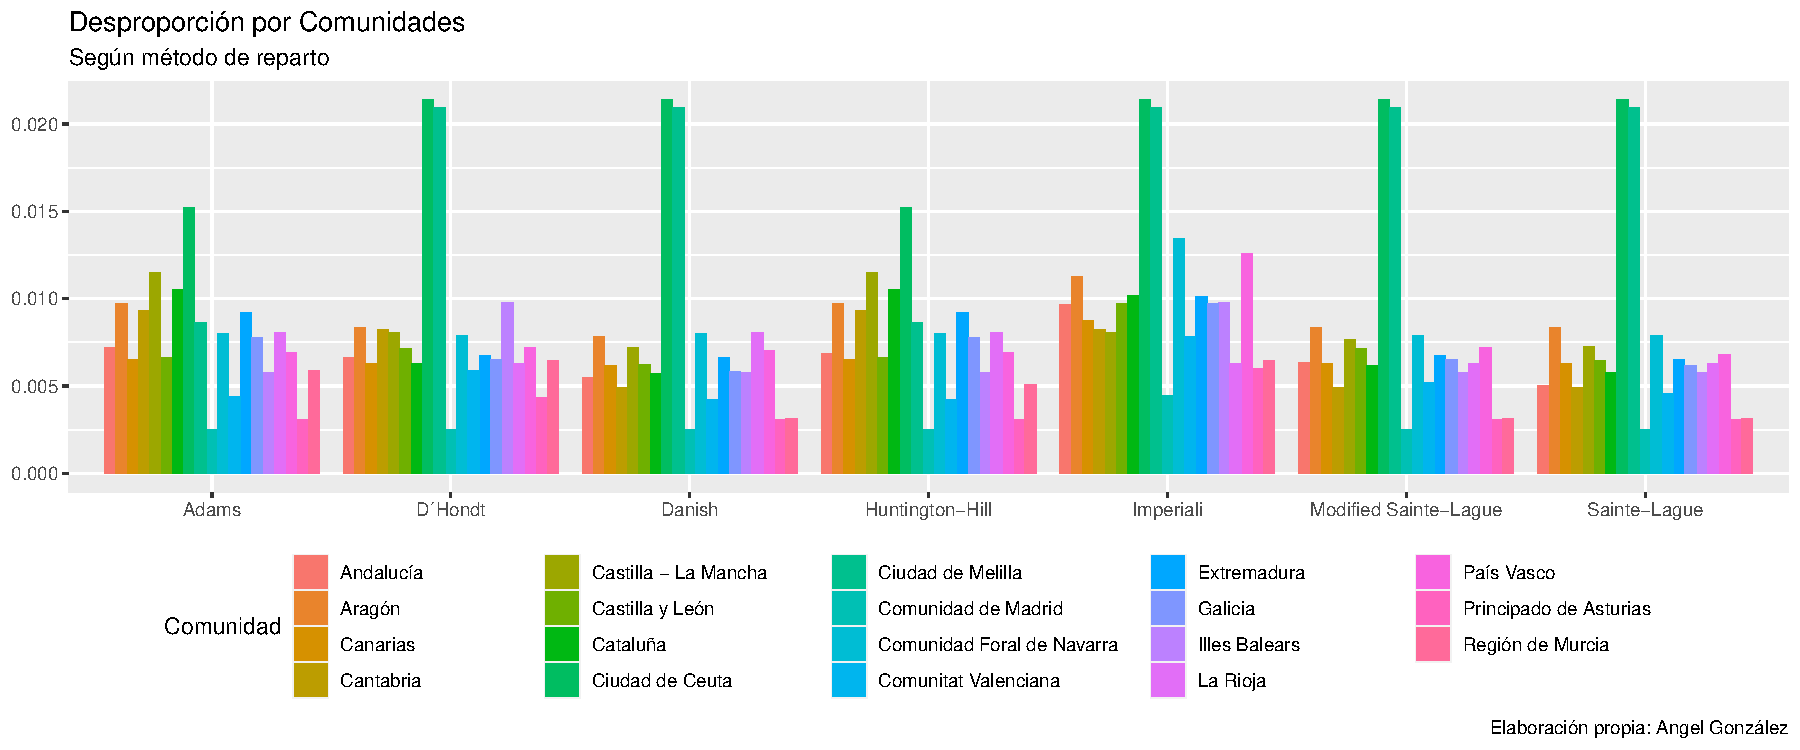
\includegraphics[width=0.95\linewidth]{figurasR/unnamed-chunk-87-1} \end{center}

\begin{center}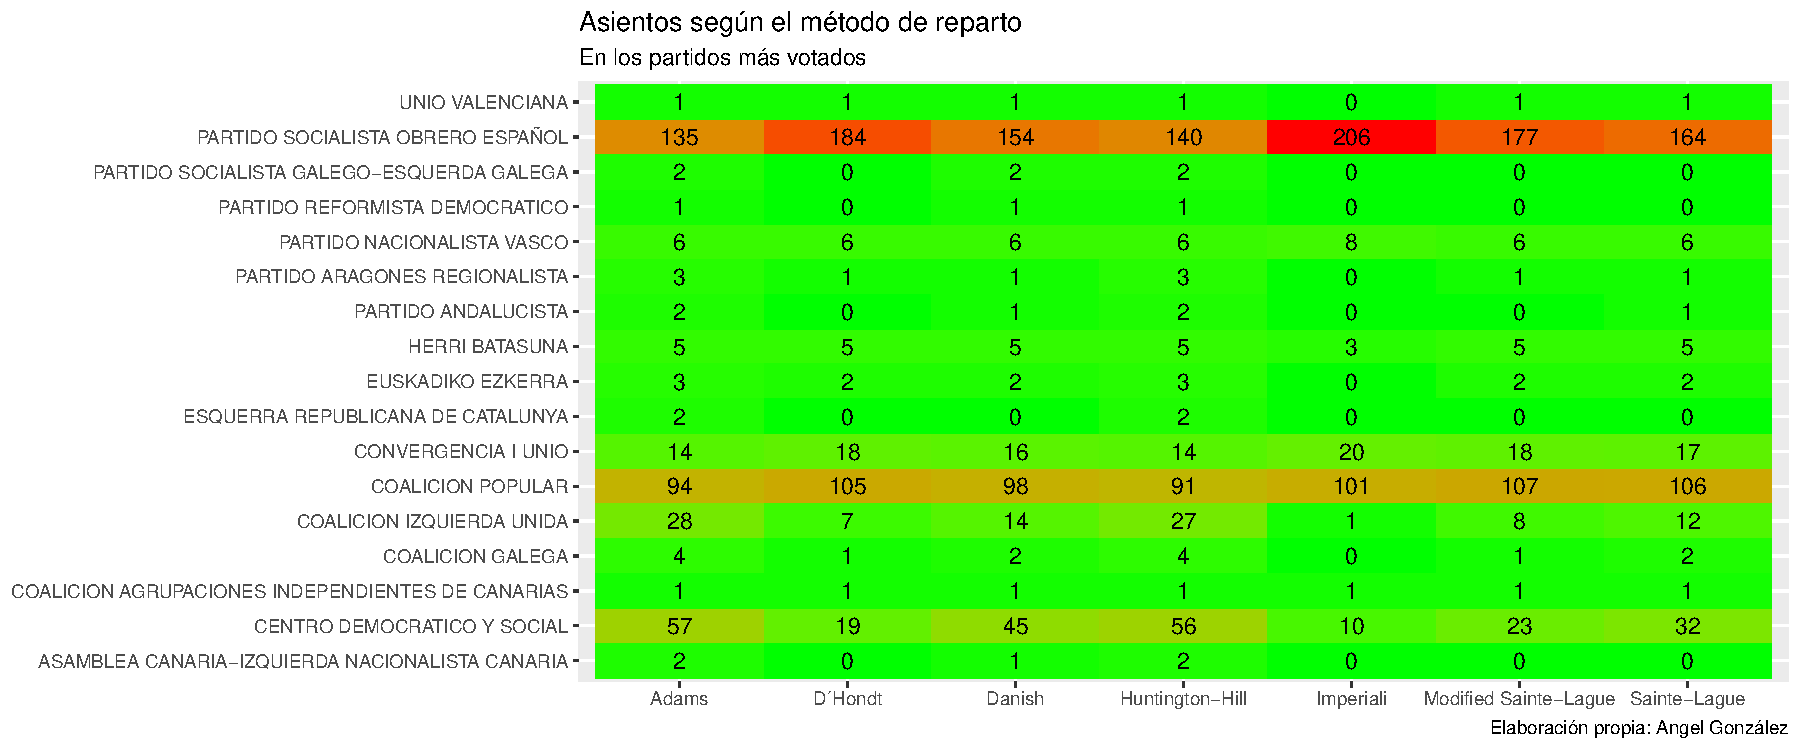
\includegraphics[width=0.95\linewidth]{figurasR/unnamed-chunk-87-2} \end{center}

Este año en el caso de la disproporción por comunidades podemos observar
que aumenta la diferencia respecto a las pasadas elecciones, una de las
comunidades más proporcionadas es la comunidad de Asturias mientras que
Aragón pasa a ser ahora una de las que más desproporción presenta. En
los extremos no hay novedades, Madrid sigue siendo la más proporcionada
y las ciudades de Ceuta y Melilla las que menos proporcionadas resultan.

Según el método de reparto este año el método Imperiali es el más
disproporcionado con diferencia, los demás métodos se podrían en un
mismo grupo, en donde el método más proporcionado este año es el método
Danish.

\hypertarget{auxf1o-1989}{%
\section{Año 1989}\label{auxf1o-1989}}

\hypertarget{comparativa-entre-muxe9todos-4}{%
\subsection{Comparativa entre
métodos}\label{comparativa-entre-muxe9todos-4}}

\hypertarget{votos-obtenidos-4}{%
\subsubsection{Votos obtenidos}\label{votos-obtenidos-4}}

\begin{center}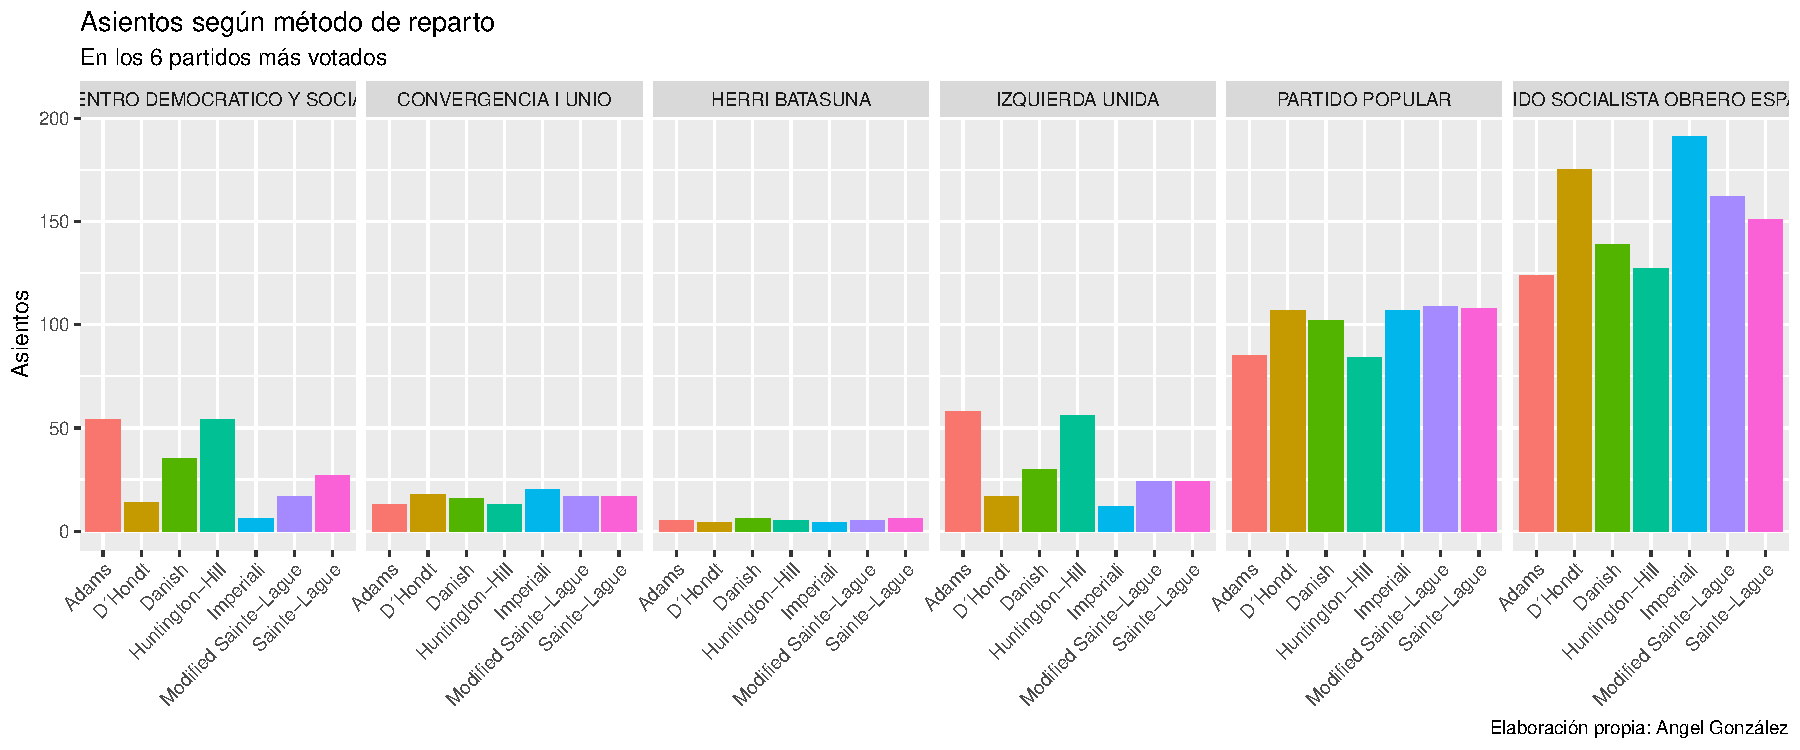
\includegraphics[width=0.95\linewidth]{figurasR/unnamed-chunk-95-1} \end{center}

\begin{center}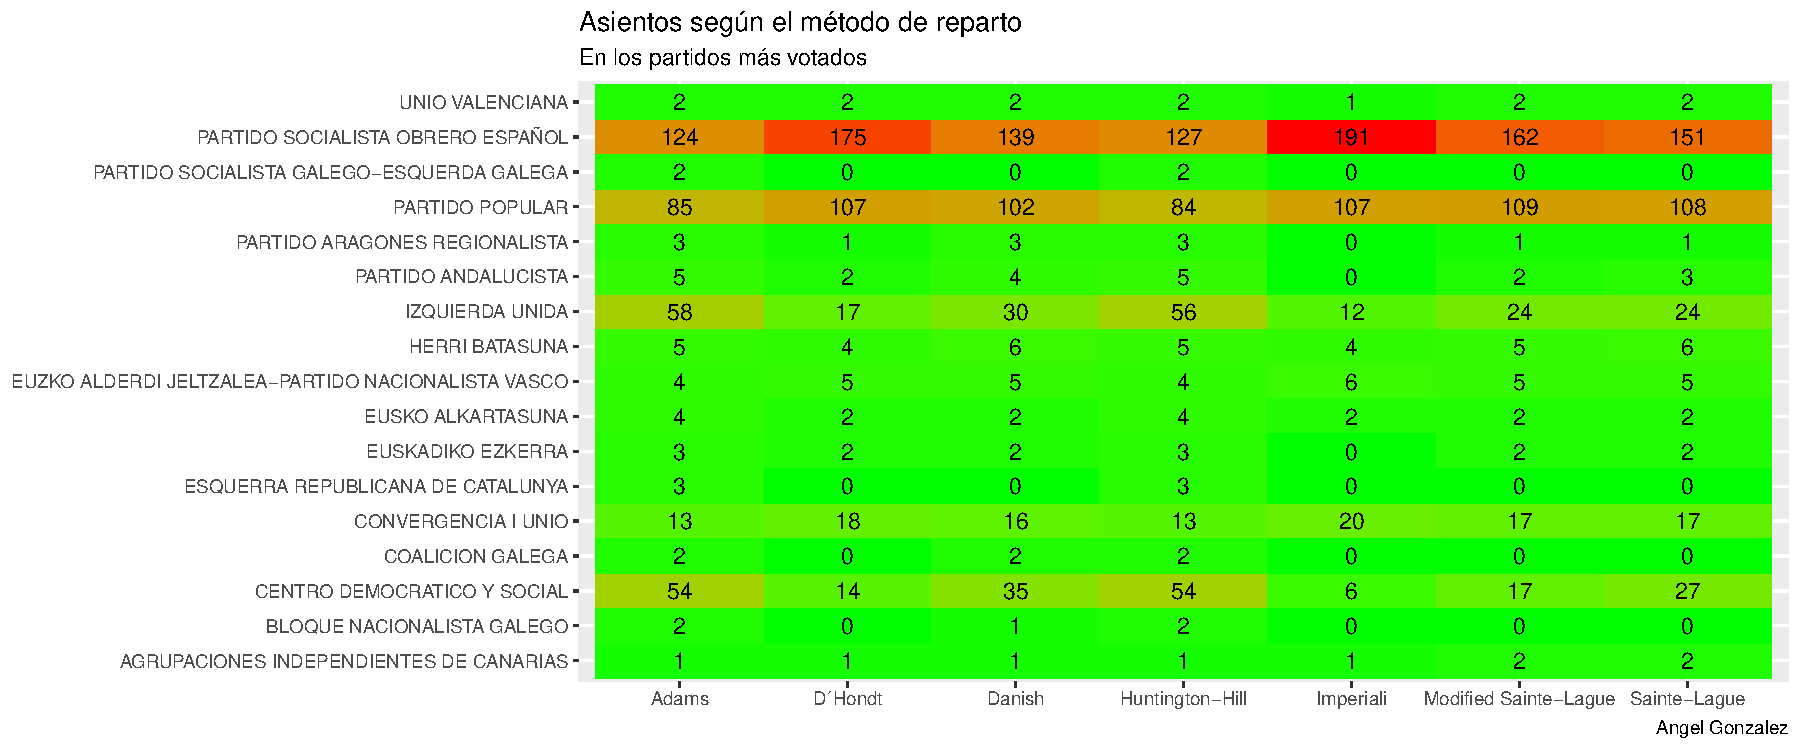
\includegraphics[width=0.95\linewidth]{figurasR/unnamed-chunk-95-2} \end{center}

En estas elecciones de 1989 el partido más votado es, como sucedió el
las anteriores elecciones, el \emph{PSOE}, vemos como aparece por
primera vez el Partido Popular como segunda fuerza tomando el puesto que
antes tenía Coalición Popular, estas elecciones también son muy
bipartidistas aunque se va debilitando ese bipartidismo, ahora podemos
decir que hay dos partidos hegemónicos, PSOE y PP, y tres partidos
medianos, los cuales serían el Centro Democrático y Social, Izquierda
Unida y Convergencia y Unión, de todos estos partidos los más
desfavorecidos por la utilización del método D´Hondt son IU y Centro
Democrático, los cuales de haber utilizado los métodos más
proporcionales podrían hasta duplicar su presencia en el congreso. Por
la otra parte en el caso del PSOE pasaría de alcanzar la mayoría
absoluta justa con 175 escaños a perder la mayoría absoluta en el caso
de optar por los métodos más proporcionales.

\hypertarget{disproporcionalidad-4}{%
\subsubsection{Disproporcionalidad}\label{disproporcionalidad-4}}

\begin{center}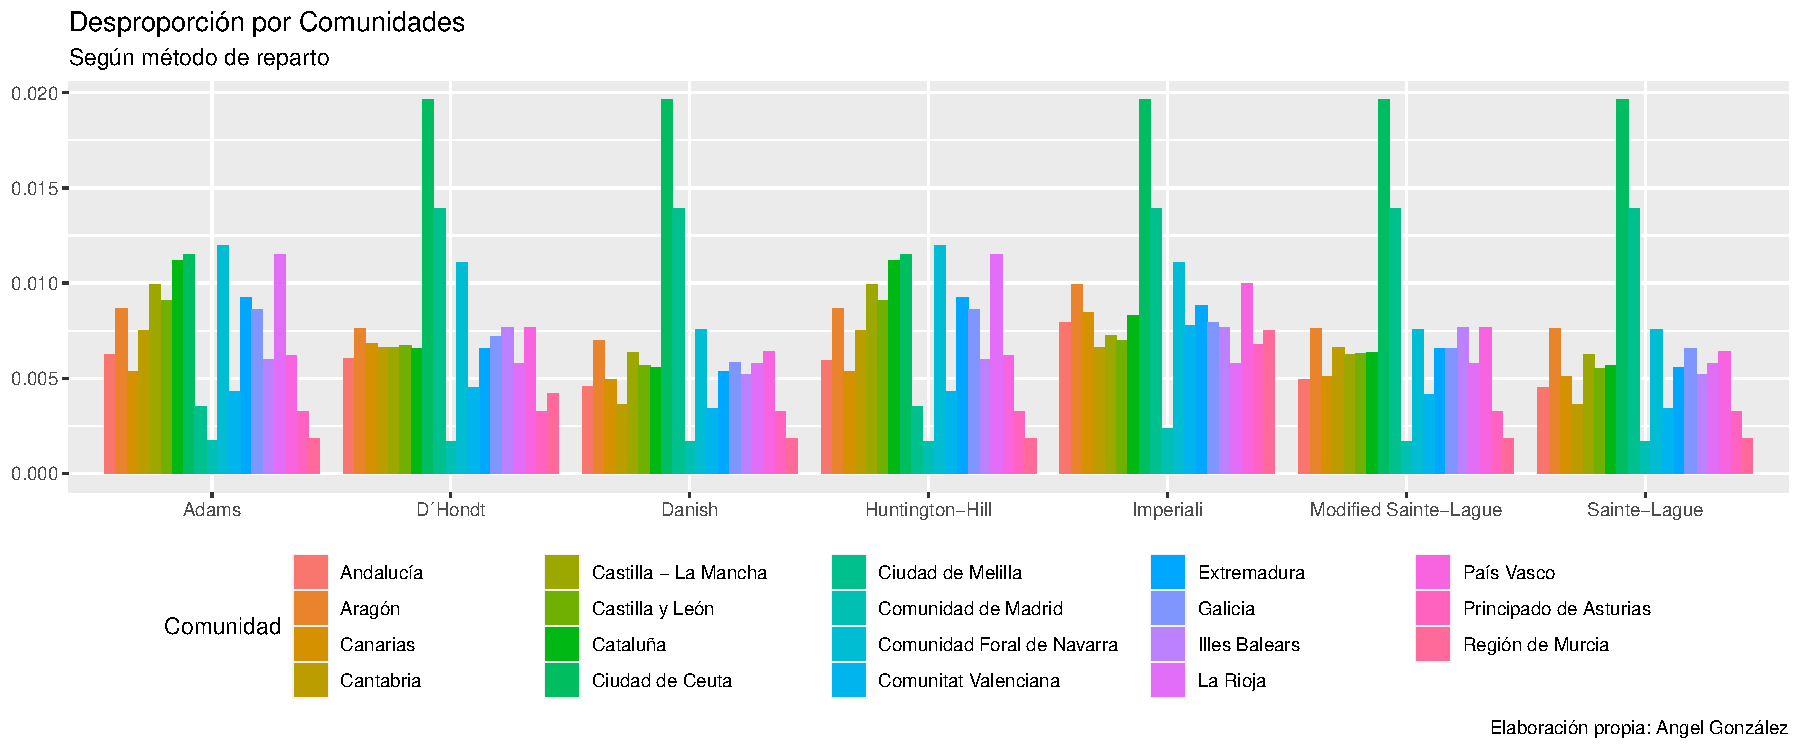
\includegraphics[width=0.95\linewidth]{figurasR/unnamed-chunk-96-1} \end{center}

\begin{center}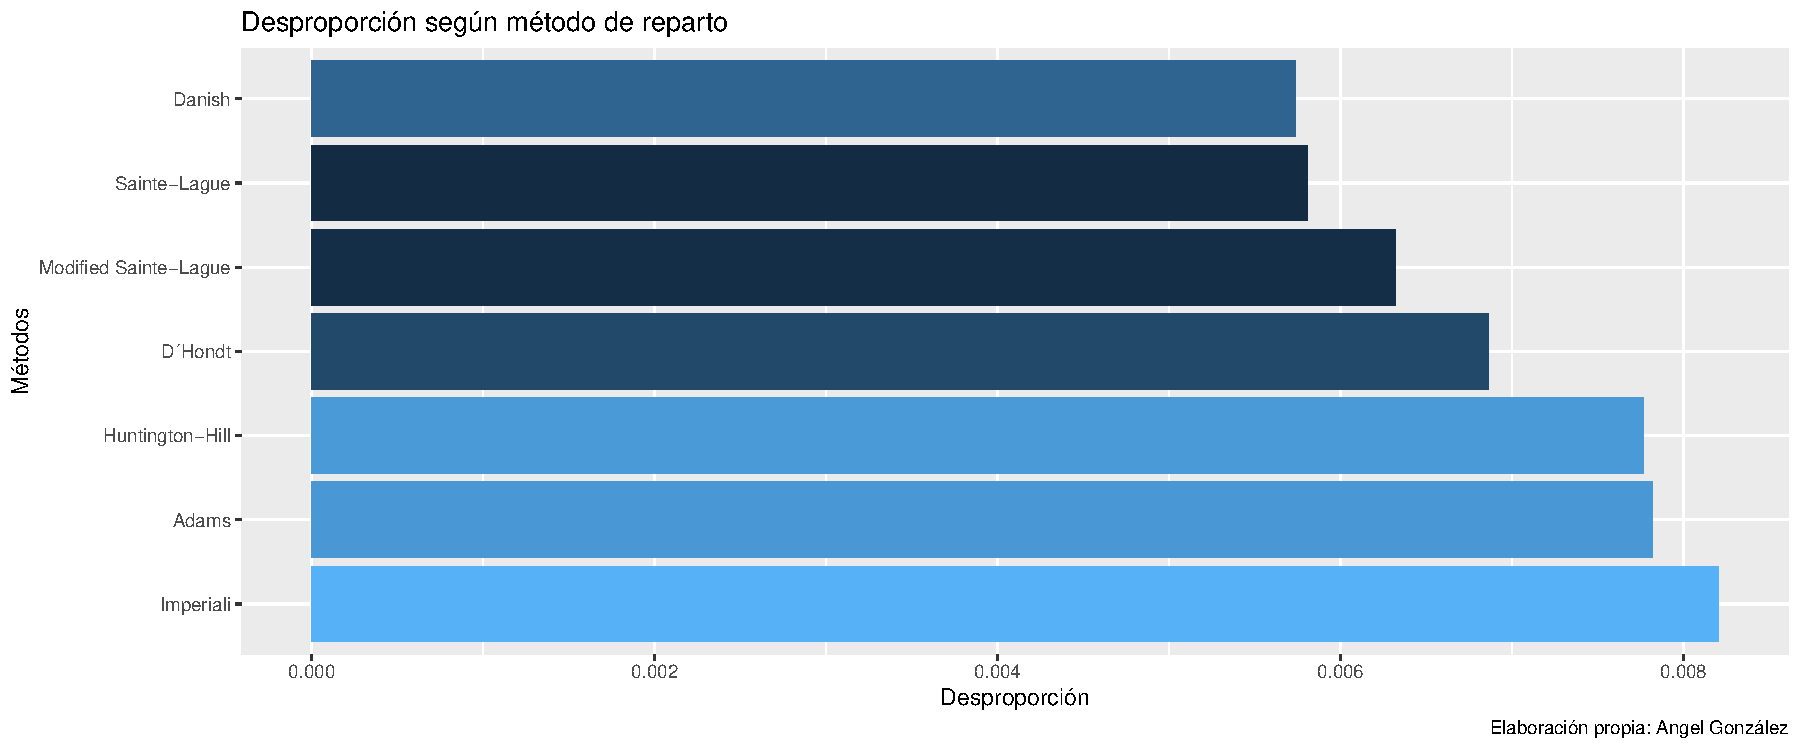
\includegraphics[width=0.95\linewidth]{figurasR/unnamed-chunk-96-2} \end{center}

Este año aunmenta ligeramente la diferencia de disproporción entre
comunidades, sin encontrar novedades en las comunidades más
proporcionales, Madrid, y las más disproporcionadas, las ciudades de
Ceuta y Melilla. Observando los métodos de reparto hay dos grupos
diferenciados, uno en el que se encuentran el método Adams y el método
de huntington-Hill, en los cuales no se encuentran comunidades con picos
de disproporción pero por el lado contrario su disproporción media es
alta, y otro grupo que serían los restantes métodos los cuales todos
presentan unos mismos picos máximos como míninos.

Estas elecciones de 1989 la disproporcionalidad media se agrupa en tres
grupos, alta, media y baja disproporción, el más disproporcionado vuelve
a ser el método Imperiali, el método D´Hondt sigue en el grupo medio y
el método más proporcionado vuelve a ser el Danish aunque le sigue muy
cerca el método Sainte-Lague.

\hypertarget{auxf1o-1993}{%
\section{Año 1993}\label{auxf1o-1993}}

\hypertarget{comparativa-entre-muxe9todos-5}{%
\subsection{Comparativa entre
métodos}\label{comparativa-entre-muxe9todos-5}}

\hypertarget{votos-obtenidos-5}{%
\subsubsection{Votos obtenidos}\label{votos-obtenidos-5}}

\begin{center}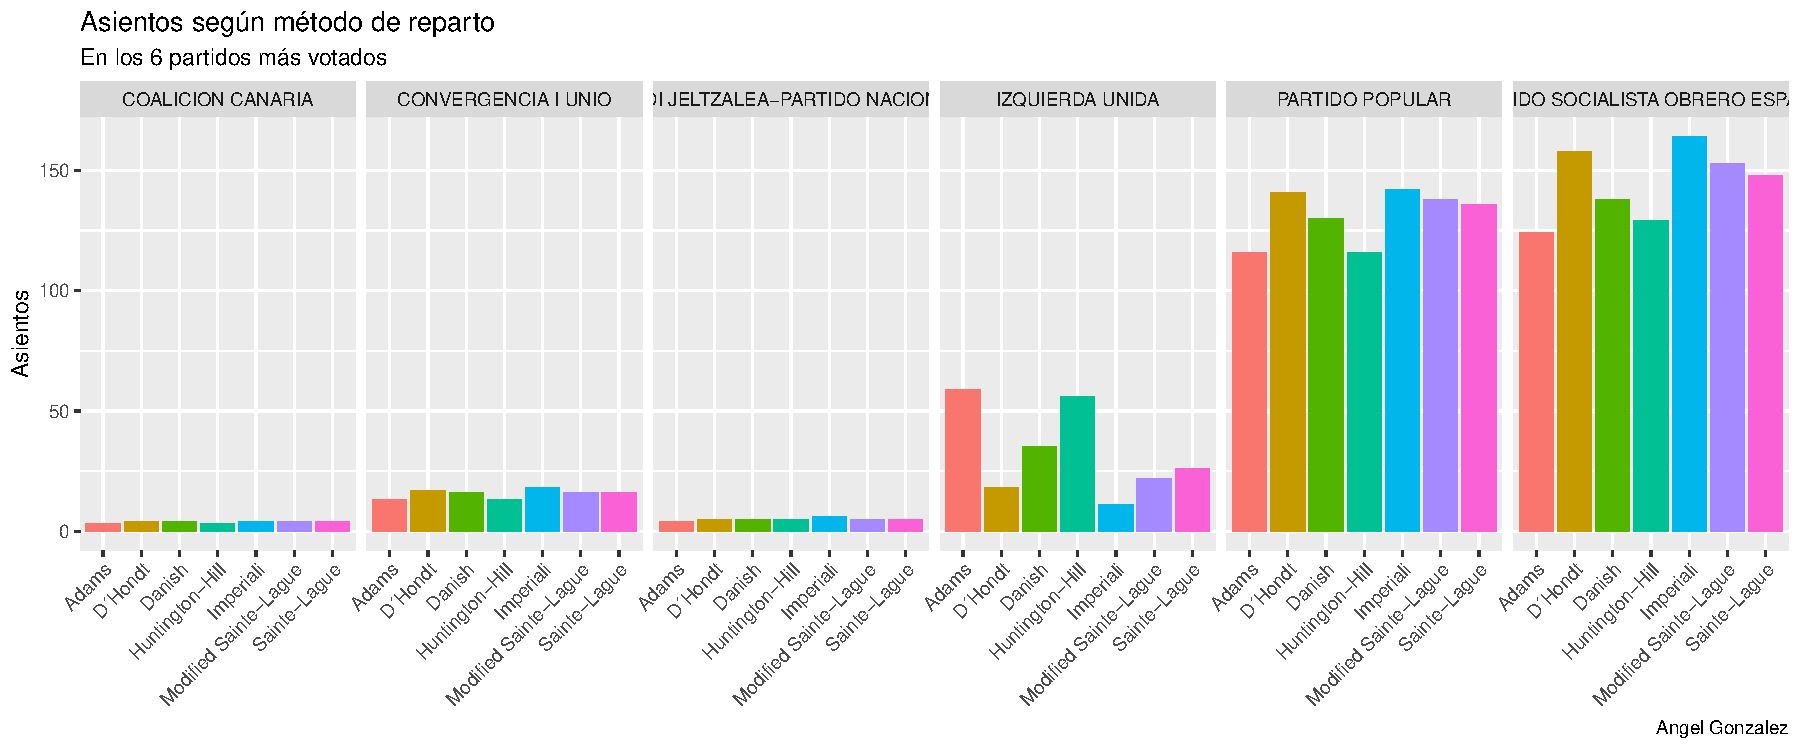
\includegraphics[width=0.95\linewidth]{figurasR/unnamed-chunk-104-1} \end{center}

\begin{center}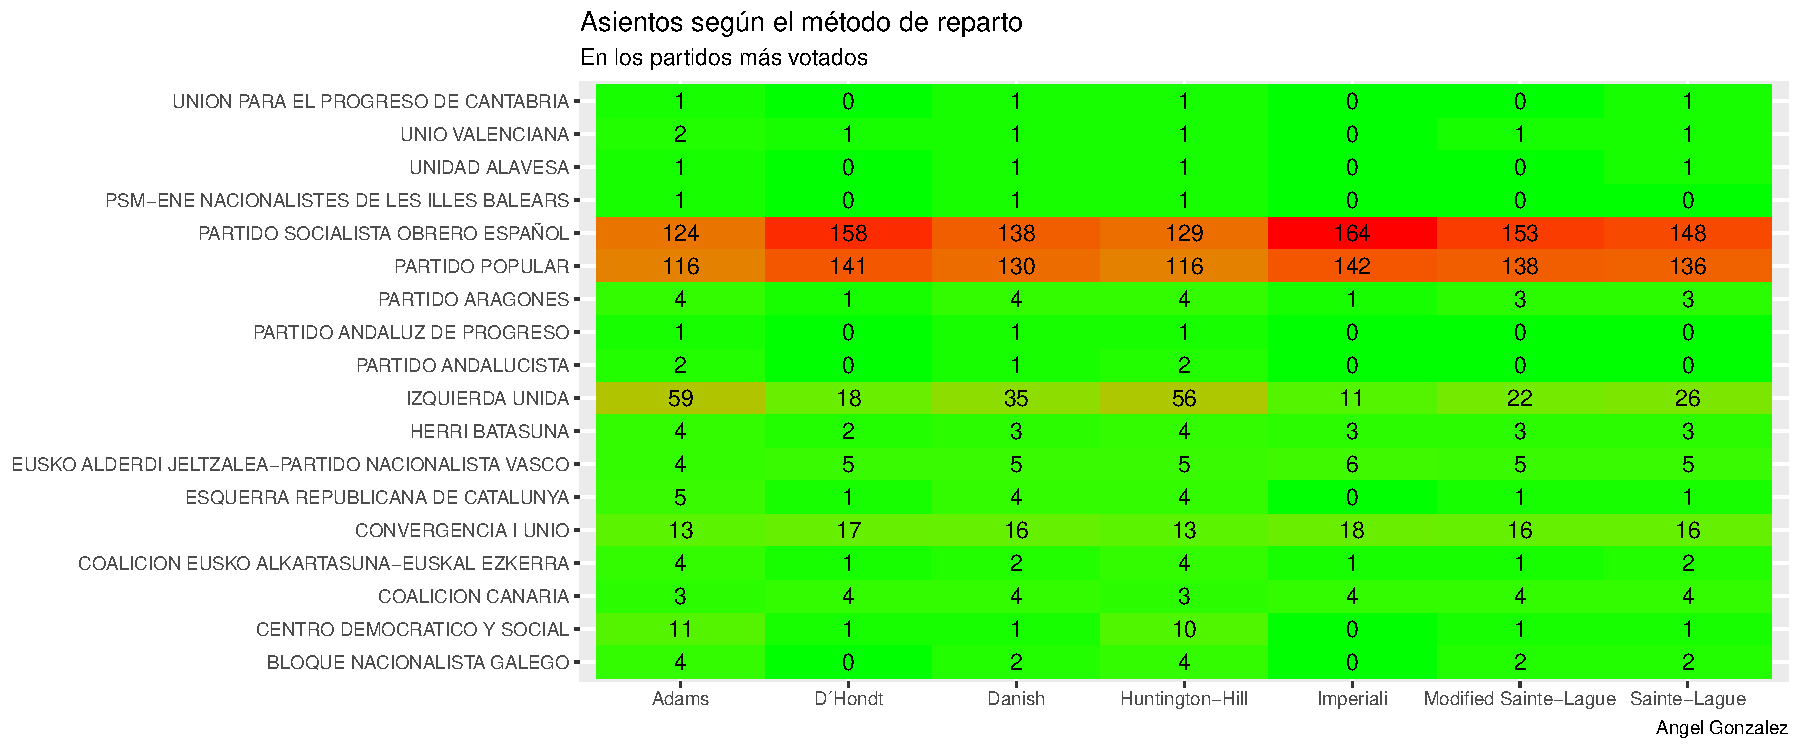
\includegraphics[width=0.95\linewidth]{figurasR/unnamed-chunk-104-2} \end{center}

En las elecciones de 1993 podemos observar como la fuerza del primer
partido va decreciendo lentamente. Los dos partidos más votados son el
\emph{PSOE} y el \emph{PP} respectivamente, la diferencia estas
elecciones es que el PSOE ha perdido la mayoría absoluta según el método
D´Hondt y en cambio el PP ha aumentado su presencia significativamente y
está ya relativamente cerca de alcanzar al PSOE. De haber utilizado los
métodos más proporcionales resultaría en una menor diferencia de escaños
entre estos dos grandes partidos, el partido más castigado en estas
elecciones sigue siendo IU, el cual podría haber obtenido de 1.5 a 2
veces más asientos de haber cambiado de método de reparto. Son unas
elecciones en donde hay dos partidos hegemónicos y dos partidos medianos
que son IU y CIU, como hemos visto IU es un partido muy castigado por el
método de reparto actual, en cambio CiU no se vería agraviado o
beneficiado al cambiar el método de reparto.

\hypertarget{disproporcionalidad-5}{%
\subsubsection{Disproporcionalidad}\label{disproporcionalidad-5}}

\begin{center}\includegraphics[width=0.95\linewidth]{figurasR/unnamed-chunk-105-1} \end{center}

\begin{center}\includegraphics[width=0.95\linewidth]{figurasR/unnamed-chunk-105-2} \end{center}

En estas elecciones se observan más picos de disproporción en
comparación con las elecciones anteriores, especialmente aumenta su
disproporción el Pais Vasco y Aragón, no hay novedades en los máximos ni
en los mínimos.

Este año en el caso de la disproporcionalidad media según el método de
reparto vemos que hay diferencias en los métodos más disproporcionales,
usualmente el método más disproporcionado ha sido el Imperiali, en estas
elecciones esto cambia, de hecho mejora en dos puestos. Los más
disproporcionados este año entonces son los métodos Adams y de
Huntington-Hill, en el caso de los más proporcionados no hay novedades,
sigue siendo el método Danish seguido muy de cerca por el Sainte-Lague.

\hypertarget{auxf1o-1996}{%
\section{Año 1996}\label{auxf1o-1996}}

\hypertarget{comparativa-entre-muxe9todos-6}{%
\subsection{Comparativa entre
métodos}\label{comparativa-entre-muxe9todos-6}}

\hypertarget{votos-obtenidos-6}{%
\subsubsection{Votos obtenidos}\label{votos-obtenidos-6}}

\begin{center}\includegraphics[width=0.95\linewidth]{figurasR/unnamed-chunk-113-1} \end{center}

\begin{center}\includegraphics[width=0.95\linewidth]{figurasR/unnamed-chunk-113-2} \end{center}

En estas elecciones de 1996 son las primeras elecciones en donde el
\emph{PP} son la fuerza más votada, el \emph{PSOE} que ya llevaba una
tendencia descendiente al final ha perdido el primer puesto. Sigue
habiendo un bipartidismo significativo con dos partidos medianos,
todavía el PP a pesar de ganar las elecciones no alcanza la mayoría
absoluta en ninguno de los métodos analizados

\hypertarget{disproporcionalidads}{%
\subsubsection{Disproporcionalidads}\label{disproporcionalidads}}

\begin{center}\includegraphics[width=0.95\linewidth]{figurasR/unnamed-chunk-114-1} \end{center}

\begin{center}\includegraphics[width=0.95\linewidth]{figurasR/unnamed-chunk-114-2} \end{center}

\hypertarget{auxf1o-2000}{%
\section{Año 2000}\label{auxf1o-2000}}

\hypertarget{comparativa-entre-muxe9todos-7}{%
\subsection{Comparativa entre
métodos}\label{comparativa-entre-muxe9todos-7}}

\hypertarget{votos-obtenidos-7}{%
\subsubsection{Votos obtenidos}\label{votos-obtenidos-7}}

\begin{center}\includegraphics[width=0.95\linewidth]{figurasR/unnamed-chunk-122-1} \end{center}

\begin{center}\includegraphics[width=0.95\linewidth]{figurasR/unnamed-chunk-122-2} \end{center}

En las elecciones del año 2000 el partido más votado vuelve a ser el
\emph{Partido Popular} seguido del \emph{PSOE}, en estas elecciones
según el método D´Hondt utilizado en España el PP conseguiría una
mayoría absoluta holgada, es una elección con un claro bipartidismo
donde se podría decir que no existen partidos medianos. Si optasemos por
otro método de reparto más proporcional como puede ser el método Danish
o el Sainte-Lague el PP no alcanzaría la mayoría absoluta, se quedaría a
muy pocos escaños de alcanzarla, en cambio veríamos a muchos partidos
pequeños con menos de tres votos casi duplicar su presencia en escaños.
El partido más castigado por utilizar el método D´Hondt en estas
elecciones sigue siendo Izquierda Unida.

\hypertarget{disproporcionalidad-6}{%
\subsubsection{Disproporcionalidad}\label{disproporcionalidad-6}}

\begin{center}\includegraphics[width=0.95\linewidth]{figurasR/unnamed-chunk-123-1} \end{center}

\begin{center}\includegraphics[width=0.95\linewidth]{figurasR/unnamed-chunk-123-2} \end{center}

Observando la disproporción por comunidades no encontramos diferencias
significativas respecto a las anteriores elecciones, es decir, tanto el
método Adams como el Huntington-Hill tienen un comportamiento diferente
respecto a los demás, siguen siendo los más despropocionados las
ciudades de Ceuta y Melilla, y la más proporcionada la Comunidad de
Madrid, este año es especialmente alta la disproporción de las Islas
Baleares respecto a anteriores elecciones.

Si miramos la gráfica de la disproporcionalidad según el método de
reparto se pueden agrupar los métodos en dos grupos, uno con gran
disproporcionalidad en el que estarían incluidos los métodos Adams,
Imperiali y Huntington-Hill, y el otro grupo restante con una
disproporción media baja. Seguimos observando que el método D´Hont no es
el mejor aunque en estas elecciones se puede considerar un método
aceptable siendo el mejor método alternativo el Danish.

\hypertarget{auxf1o-2004}{%
\section{Año 2004}\label{auxf1o-2004}}

\hypertarget{comparativa-entre-muxe9todos-8}{%
\subsection{Comparativa entre
métodos}\label{comparativa-entre-muxe9todos-8}}

\hypertarget{votos-obtenidos-8}{%
\subsubsection{Votos obtenidos}\label{votos-obtenidos-8}}

\begin{center}\includegraphics[width=0.95\linewidth]{figurasR/unnamed-chunk-131-1} \end{center}

\begin{center}\includegraphics[width=0.95\linewidth]{figurasR/unnamed-chunk-131-2} \end{center}

En estas elecciones del año 2004 volvemos a ver unas elecciones con un
claro bipartidismo y con una diferencia de escaños entre partidos cada
vez menor, en estas elecciones el partido más votado cambia y el
\emph{PSOE} obtiene los mayores votos, seguido del \emph{PP} que pierde
la mayoría absoluta según D´Hont que tenía en las anteriores elecciones.
En ningún método el PSOE alcanzaría la mayoría absoluta por lo que
deberá de realizar alianzas con otros partidos para así alcanzar la
mayoría absoluta, si optásemos por los métodos mas proporcionales
veríamos una reducción muy significativa de la diferencia de escaños
entre partidos que pasaría de una diferencia de 16 escaños a 6 escaños
en el caso de optar por el método Danish, en cambio el partido más
castigado por el método D´Hondt, Izquierda Unida, hasta podría ver
duplicado o triplicado su presencia en el congreso.

\hypertarget{disproporcionalidad-7}{%
\subsubsection{Disproporcionalidad}\label{disproporcionalidad-7}}

\begin{center}\includegraphics[width=0.95\linewidth]{figurasR/unnamed-chunk-132-1} \end{center}

\begin{center}\includegraphics[width=0.95\linewidth]{figurasR/unnamed-chunk-132-2} \end{center}

Según el gráfico anterior por comunidades sigue la tónica general de las
anteriores elecciones, únicamente podemos apreciar en estas elecciones
una reducción de la disproporciorcionalidad entre comunidades, es decir,
una menor diferencia de disproporcionalidad entre ellas. En el caso de
agrupar la disproporción por métodos observamos que el método Imperiali
vuelve a ser el más disproporcionado este año mientras que en la parte
de los métodos mas proporcionados el método mejor sería el Sainte-Lague,
el método utilizado en España sigue siendo un método que se encuentra en
el medio, no siendo ni bueno ni malo.

\hypertarget{auxf1o-2008}{%
\section{Año 2008}\label{auxf1o-2008}}

\hypertarget{comparativa-entre-muxe9todos-9}{%
\subsection{Comparativa entre
métodos}\label{comparativa-entre-muxe9todos-9}}

\hypertarget{votos-obtenidos-9}{%
\subsubsection{Votos obtenidos}\label{votos-obtenidos-9}}

\begin{center}\includegraphics[width=0.95\linewidth]{figurasR/unnamed-chunk-140-1} \end{center}

\begin{center}\includegraphics[width=0.95\linewidth]{figurasR/unnamed-chunk-140-2} \end{center}

En estos comicios del año 2008 no hay diferencias significativas en
términos de escaños, sigue un claro bipartidismo con dos partidos
hegemónicos, en primer lugar el más votado en estas elecciones que sigue
siendo el \emph{PSOE} seguido por el \emph{PP}, la diferencia de escaños
entre ellos continúa siendo prácticamente la misma pero en este año el
bipartidismo es cada vez más pronunciado, aumentando ambos partidos su
presencia en el congreso. Para el partido más votado únicamente en un
caso podría obtener la mayoría absoluta, que sería en el caso de optar
por el método Imperiali, una mayoría absoluta justa al llegar sólo a los
175 escaños. Utilizando los métodos de reparto más proporcionales como
son el Danish y el Sainte-Lague la diferencia entre los partidos más
votados se reduciría a la vez que obtendrían un menor número de escaños,
el partido más perjudicado sigue siendo Izquierda Unida que podría en
este año hasta mas que quintuplicar su presencia en el congreso de haber
optado por el método Danish.

\hypertarget{disproporcionalidad-8}{%
\subsubsection{Disproporcionalidad}\label{disproporcionalidad-8}}

\begin{center}\includegraphics[width=0.95\linewidth]{figurasR/unnamed-chunk-141-1} \end{center}

\begin{center}\includegraphics[width=0.95\linewidth]{figurasR/unnamed-chunk-141-2} \end{center}

Este es un año que se puede observar una mayor igualdad en el caso de
las disproporcionalidades, las comunidades no tienen una gran diferencia
de proporcionalidad entre ellas y además no encontramos grandes
diferencias entre los métodos. Si observamos la gráfica de la
disproporcionalidad según el método de reparto es llamativo este año que
únicamente tenemos un método especialmente dispropocionado que es el
Imperiali, en cambio todos los demás métodos están en un mismo nivel con
una baja diferencia entre ellos, el mejor método en estas elecciones
vuelve a ser el método de Sainte-Lague, el método D´Hont utilizado en
España no presenta diferencias y se encuentra en un nivel medio-alto de
disproporcionalidad entre todos los métodos analizados.

\hypertarget{auxf1o-2011}{%
\section{Año 2011}\label{auxf1o-2011}}

\hypertarget{comparativa-entre-muxe9todos-10}{%
\subsection{Comparativa entre
métodos}\label{comparativa-entre-muxe9todos-10}}

\hypertarget{votos-obtenidos-10}{%
\subsubsection{Votos obtenidos}\label{votos-obtenidos-10}}

\begin{center}\includegraphics[width=0.95\linewidth]{figurasR/unnamed-chunk-149-1} \end{center}

\begin{center}\includegraphics[width=0.95\linewidth]{figurasR/unnamed-chunk-149-2} \end{center}

Este año 2011 podemos considerarlo como el primer año en el que aunque
siga sucediendo un claro bipartidismo empiezan a surgir partidos
medianos con cada vez más presencia en el congreso, en este año es la
aparición de UPyD. El partido más votado en estas elecciones es el
Partido Popular, que además obtiene la mayoría absoluta de forma holgada
según el método D´Hondt utilizado en España, le sigue el PSOE a una
diferencia muy significativa, casi duplica la presencia en el congreso
del PP respecto al PSOE. Si observamos los otros métodos propuestos
vemos que el PP en el caso del método Danish no llegaría a obtener la
mayoría absoluta pero si utilizásemos el método de Sainte-Lague sí que
alcanzaríamos la mayoría absoluta con 176 escaños. Los partidos más
perjudicados por utilizar el método D´Hont son en estas elecciones UPyD
y IU, los cuales de haber optado por el método Danish podrían duplicar
su presencia en el congreso. Es llamativo el resultado de las elecciones
según el método Adams y Huntington-Hill, son métodos que dan escaños a
los partidos con menos votos en detrimento de los partidos más votados,
en estas elecciones vemos como el resultado cambiaría radicalmente, el
PP de ser el partido más votado con mucha diferencia pasaría a reducir
la diferencia de escaños a la mitad pero la diferencia más notoria está
en los partidos medianos UPyD y IU, que pasarían de 5 a 41 escaños y de
11 a 54 escaños respectivamente.

\hypertarget{disproporcionalidad-9}{%
\subsubsection{Disproporcionalidad}\label{disproporcionalidad-9}}

\begin{center}\includegraphics[width=0.95\linewidth]{figurasR/unnamed-chunk-150-1} \end{center}

\begin{center}\includegraphics[width=0.95\linewidth]{figurasR/unnamed-chunk-150-2} \end{center}

Observando el gráfico de la disproporcionalidad entre comunidades vemos
como este año particularmente el comportamiento general de todos los
métodos es similar a diferencia de las anteriores elecciones en donde
los métodos Adams y Huntington-Hill presentaban un comportamiento
distinto respecto a los restantes métodos, este año el comportamiento de
todos los métodos es similar.

Si observamos la disproporcionalidad según el método de reparto volvemos
a observar dos grupos bien diferenciados, uno en el que hay una gran
disproporcionalidad, donde estarían los métodos Huntington-Hill, Adams e
Imperiali, y otro grupo con los restantes métodos con una
proporcionalidad baja. El método utilizado en España se encontraría en
el grupo de disproporcionalidad baja pero con el inconveniente de ser el
peor clasificado en ese grupo, el mejor método estas elecciones es el
Danish.

\hypertarget{auxf1o-2015}{%
\section{Año 2015}\label{auxf1o-2015}}

\hypertarget{comparativa-entre-muxe9todos-11}{%
\subsection{Comparativa entre
métodos}\label{comparativa-entre-muxe9todos-11}}

\hypertarget{votos-obtenidos-11}{%
\subsubsection{Votos obtenidos}\label{votos-obtenidos-11}}

\begin{center}\includegraphics[width=0.95\linewidth]{figurasR/unnamed-chunk-158-1} \end{center}

\begin{center}\includegraphics[width=0.95\linewidth]{figurasR/unnamed-chunk-158-2} \end{center}

En estas elecciones del 2014 ya vemos como habíamos predicho en las
anteriores que el bipartidismo que veíamos omnipresente en todas las
elecciones anteriores ahora ya no ocurre, es el primer año en el que se
puede afirmar que ya no hay bipartidismo. El partido más votado es el
\emph{Partido Popular} seguido por el \emph{PSOE}, pero ya vemos que
este año aparecen dos nuevos partidos medianos, que son Podemos y
Ciudadanos. El partido más votado no obtiene la mayoría absoluta en
ningún método, es interesante observar como entre Podemos y Ciudadanos
en el caso de utilizar el método D´Hondt el primero superaría en dos
escaños al segundo, mientras que de haber utilizado el método Danish
Ciudadanos superaría a Podemos en dos escaños. En el caso de optar por
el método Danish el partido más votado, el PP, perdería bastantes
escaños y su diferencia respecto al segundo se vería reducida
significativamente, en el caso de los partidos medianos verían su
presencia en el congreso aumentar levemente pero en ningún caso
supondría un cambio significativo. El partido más perjudicado este año
vuelve a ser Izquierda Unida, que podría pasar de obtener 2 escaños con
el método D´Hondt a 11 escaños con el Danish.

\hypertarget{disproporcionalidad-10}{%
\subsubsection{Disproporcionalidad}\label{disproporcionalidad-10}}

\begin{center}\includegraphics[width=0.95\linewidth]{figurasR/unnamed-chunk-159-1} \end{center}

\begin{center}\includegraphics[width=0.95\linewidth]{figurasR/unnamed-chunk-159-2} \end{center}

Según el gráfico por comunidades volvemos a ver un comportamiento
claramente distinto de los demás de los métodos Adams y Huntington-Hill,
es un año en el que la diferencia de disproporcionalidad entre las
distintas comunidades aumentan.

En el caso de la disproporción según el método de reparto este año
tenemos nuevamente dos grupos difenrenciados, en un grupo con una
disproporcionalidad alta estaría únicamente el método Imperiali y todos
los métodos restantes se encontrarían en el grupo de disproporcionalidad
baja, el mejor método este año es el Sainte-Lague y encontramos que el
método utilizado en España es el segundo peor método posible, por lo
tanto sería interesante este año utilizar otro método mejor.

\hypertarget{auxf1o-2016}{%
\section{Año 2016}\label{auxf1o-2016}}

\hypertarget{comparativa-entre-muxe9todos-12}{%
\subsection{Comparativa entre
métodos}\label{comparativa-entre-muxe9todos-12}}

\hypertarget{votos-obtenidos-12}{%
\subsubsection{Votos obtenidos}\label{votos-obtenidos-12}}

\begin{center}\includegraphics[width=0.95\linewidth]{figurasR/unnamed-chunk-167-1} \end{center}

\begin{center}\includegraphics[width=0.95\linewidth]{figurasR/unnamed-chunk-167-2} \end{center}

En las elecciones del año 2016 vemos como se va consolidando el modelo
de las anteriores elecciones, con dos grandes partidos y dos partidos
medianos. La fuerza política más votada este año es el \emph{Partido
Popular} seguido del \emph{PSOE}, en ningún método el PP alcanzaría la
mayoría absoluta, son unas elecciones que no presentan diferencias
significativas al cambiar de método de reparto, en el caso de utilizar
el método Danish respecto al D´Hondt resultaría en un menor número de
escaños para el PP y una ligera subida de escaños de Podemos y
Ciudadanos. Son las primeras elecciones en donde el método de reparto no
cambia significativamente el reparto de escaños, es notorio que en este
año el PSOE obtenga casi los mismos votos independientemente del método
utilizado.

\hypertarget{disproporcionalidad-11}{%
\subsubsection{Disproporcionalidad}\label{disproporcionalidad-11}}

\begin{center}\includegraphics[width=0.95\linewidth]{figurasR/unnamed-chunk-168-1} \end{center}

\begin{center}\includegraphics[width=0.95\linewidth]{figurasR/unnamed-chunk-168-2} \end{center}

En la disproporcionalidad por comunidades vemos el habitual
comportamiento entre los métodos, con el método Adams y el
Huntington-Hill comportándose diferente a los demás. Respecto a las
diferencias de disproporcionalidad entre comunidades este año es
especialmente similar el comportamiento entre los distintos métodos. En
el gráfico en que comparamos los métodos de reparto el comportamiento es
similar al anterior año, con un método muy disproporcional respecto a
los demás, el método Imperiali, y los demás métodos muy similares entre
ellos siendo el mejor el método de Sainte-Lague, el método utilizado en
España, el D´Hondt, vuelve a ser el segundo peor por lo que cada vez es
más necesario proponer un cambio de método de reparto a otro más
proporcional.

\hypertarget{auxf1o-2019-abril}{%
\section{Año 2019, Abril}\label{auxf1o-2019-abril}}

\hypertarget{comparativa-entre-muxe9todos-13}{%
\subsection{Comparativa entre
métodos}\label{comparativa-entre-muxe9todos-13}}

\hypertarget{votos-obtenidos-13}{%
\subsubsection{Votos obtenidos}\label{votos-obtenidos-13}}

\begin{center}\includegraphics[width=0.95\linewidth]{figurasR/unnamed-chunk-176-1} \end{center}

\begin{center}\includegraphics[width=0.95\linewidth]{figurasR/unnamed-chunk-176-2} \end{center}

En estas elecciones de Abril de 2019 vemos como ya no existe
bipartidismo, este año podemos agrupar a los partidos políticos en
cuatro categorías, la primera en donde hay un partido con muchos votos
con una gran diferencia de escaños respecto a los demás, que es el PSOE,
un segundo grupo en donde se encontrarían dos partidos con un número
medio-alto de escaños, que son el PP y Ciudadanos respectivamente, un
tercer grupo con un número mediano de escaños con Podemos y Vox, y un
último grupo de pocos escaños con los demás partidos. Este año tampoco
hay una diferencia significativa de haber utilizado un método de reparto
respecto a otro, no hay partidos especialmente perjudicados por la
elección del método D´Hondt, en ningún caso el partido más votado
alcanza la mayoría absoluta. De haber utilizado el método Danish el
partido que se vería más beneficiado sería Vox seguido de Ciudadanos,
partido que superaría en escaños al PP y se convertiría en la segunda
fuerza en el hemiciclo.

\hypertarget{disproporcionalidad-12}{%
\subsubsection{Disproporcionalidad}\label{disproporcionalidad-12}}

\begin{center}\includegraphics[width=0.95\linewidth]{figurasR/unnamed-chunk-177-1} \end{center}

\begin{center}\includegraphics[width=0.95\linewidth]{figurasR/unnamed-chunk-177-2} \end{center}

Este es un año en el que viendo la disproporcionalidad por comunidades
es especialmente similar independientemente del método utilizado, todos
los métodos siguen un patrón de disproporcionalidad similar, sin olvidar
el comportamiento habitual de las ciudades de Ceuta y Melilla y de la
comunidad de Madrid como la provincia más proporcionada.

Cuando comparamos la proporcionalidad según el método de reparto sucede
algo que no se había visto hasta ahora, que un método que anteriormente
a llegado a ser el más disproporcionado sucede que este año es el más
proporcionado, este método es el Huntington-Hill, en el extremo opuesto
está el método Imperiali con una diferencia bastante significativa
respecto a las demás. El método utilizado en España vuelve a ser uno de
los peores, en estas elecciones el segundo peor, parece ser un método
que no está preparado para ser óptimo en escenarios en donde no hay un
bipartidismo claro.

\hypertarget{auxf1o-2019-noviembre}{%
\section{Año 2019, Noviembre}\label{auxf1o-2019-noviembre}}

\hypertarget{comparativa-entre-muxe9todos-14}{%
\subsection{Comparativa entre
métodos}\label{comparativa-entre-muxe9todos-14}}

\hypertarget{votos-obtenidos-14}{%
\subsubsection{Votos obtenidos}\label{votos-obtenidos-14}}

\begin{center}\includegraphics[width=0.95\linewidth]{figurasR/unnamed-chunk-185-1} \end{center}

\begin{center}\includegraphics[width=0.95\linewidth]{figurasR/unnamed-chunk-185-2} \end{center}

En esta gráfica de las elecciones de Noviembre de 2019 podemos observar
una ligera recuperación del bipartidismo en donde los dos principales
partidos vuelven a aumentar el número de escaños obtenidos y también
aumentar la diferencia en escaños respecto a los demás. Son unas
elecciones en donde hay dos partidos principales, que son el \emph{PSOE}
y el \emph{PP} respectivamente, uno medio en escaños, \emph{Vox}, y tres
partidos de un nivel medio-bajo de escaños, que son \emph{Podemos},
\emph{ERC} y \emph{Ciudadanos} respectivamente. En el caso de optar por
otro método en ninguno de ellos se alcanzaría la mayoría absoluta, hay
dos partidos perjudicados por utilizar el método D´Hondt en vez de otro
más proporcional como pueda ser el Danish, que son los partidos de
Podemos que pasarían de obtener 26 escaños a 40 y el partido Ciudadanos
que pasaría a duplicar su presencia de 10 escaños a 23.

\hypertarget{disproporcionalidad-13}{%
\subsubsection{Disproporcionalidad}\label{disproporcionalidad-13}}

\begin{center}\includegraphics[width=0.95\linewidth]{figurasR/unnamed-chunk-186-1} \end{center}

\begin{center}\includegraphics[width=0.95\linewidth]{figurasR/unnamed-chunk-186-2} \end{center}

En el gráfico por comunidades obtenemos el mismo comportamiento que en
las elecciones anteriores sin obtener una diferencia significativa.
Cuando comparamos la disproporcionalidad según el método de reparto el
método de Imperiali sigue siendo el más disproporcionado mientras que el
mejor método esta vez resulta ser el Sainte-Lague, el método D´Hondt
como hemos visto en anteriores elecciones sigue siendo el segundo peor
método posible, por lo que es necesario cada vez más plantear seriamente
un cambio de método de reparto.

\hypertarget{comparativa-entre-auxf1os}{%
\section{Comparativa entre años}\label{comparativa-entre-auxf1os}}

\begin{center}\includegraphics[width=0.95\linewidth]{figurasR/unnamed-chunk-187-1} \end{center}

\begin{center}\includegraphics[width=0.95\linewidth]{figurasR/unnamed-chunk-187-2} \end{center}

En este gráfico comparando la disproporcionalidad media por año
observamos como la disproporción desde las elecciones de 1977 hasta 1989
está en un nivel medio, a partir del año 1993 la disproporción baja,
principalmente debido a un bipartidismo más marcado, esto se mantiene
hasta el año de las elecciones de 2011, en donde empieza por primera vez
a aparecer un tercer partido que debilita el bipartidismo por lo que la
disproporcionalidad aumenta a los niveles de las primeras elecciones,
desde el año 2011 hasta ya las últimas elecciones de 2019 la
disproporcionalidad se mantiene sin mucha variación.

En el gráfico de la disproporcionalidad según el método de reparto
podemos extraer conclusiones para decidir cual método ha sido el mejor a
lo largo de todas las elecciones realizadas en España a partir de 1977,
por lo tanto sacamos estas conclusiones:

\begin{itemize}
\tightlist
\item
  El mejor método es el Saint-Lague.
\item
  El peor método es el Imperiali.
\item
  El método D´Hondt es el cuarto mejor método.
\end{itemize}

Por lo tanto al preguntarnos si el método utilizado en España es el
mejor método que se puede utilizar para el reparto de los escaños
podemos afirmar que no lo es, de hecho se sitúa en la mitad de la tabla
entre todos los métodos analizados, la característica que tiene el
método D´Hont es que se sitúa entre los métodos que benefician más a los
partidos más votados y de entre ellos es el método más proporcional, por
lo que se podría decir que es el método más proporcional entre los
métodos que ``facilitan la gobernanza''. Pero si nuestro objetivo es
obtener la máxima proporcionalidad en vez de facilitar la gobernanza
deberíamos plantear un cambio de método en primer lugar al Sainte-Lague
o al Danish, ambos métodos son casi idénticos en términos de
proporcionalidad pero el Sainte-Lague tiene una mejor característica que
el Danish, que reparte los escaños de forma que es más fácil gobernar.

--\textgreater{}

\FloatBarrier
\cleardoublepage

\ifdefined\ifdoblecara
  \fancyhead[LE,RO]{}
  \fancyfoot[LO,RE]{}
  \fancyhead[CO,CE]{Bibliografía}
\else
  \fancyhead[RO]{}
  \fancyfoot[LO]{}
  \fancyhead[CO]{Bibliografía}
\fi

\ifdefined\ifcitapandoc

\hypertarget{bibliografuxeda}{%
\chapter*{Bibliografía}\label{bibliografuxeda}}
\addcontentsline{toc}{chapter}{Bibliografía}

\else

\nocite{*}

\fi

\bibliography{bib/library.bib,bib/paquetes.bib}


\addcontentsline{toc}{chapter}{Bibliografía}


\end{document}
